\chapter{Anwendung: Oberflächenkrümmung}
  
  \begin{ziel}
    In vielen wissenschaftlichen Problemen kann die Krümmung
    einer Oberfläche eine entscheidende Rolle spielen. 
    Sie kann zum Beispiel ein wichtiger Bestandteil von Differentialgleichungen sein.
    So kommt die mittlere Krümmung \( H \) bei fluidmechanischen Formulierungen auf bewegliche Membranen 
    \( M_{t} \) in der
    Kontinuitätsgleichung
    \begin{align}
      \dot{\rho} + \rho\div\vec{v} - \rho v_{\vec{\nu}} H &= 0
    \end{align}
    vor (siehe \cite{desimone}).
    Ein weiteres einfaches Beispiel ist die Evolution von Oberflächen \( M_{t} \) über den mittleren
    Krümmungsfluss
    \begin{align}
      \dot{\vec{x}} = 2 H \vec{\nu} 
    \end{align}
    oder die Bestimmung des topologisch invarianten Geschlechts
    \begin{align}
      \mathfrak{g} = 1 - \frac{1}{4\pi}\int_{M}K\mu
    \end{align}
    einer orientierten Mannigfaltigkeit \( M \) ohne Rand mit Gaußscher Krümmung \( K \),
    was direkt aus dem Satz von Gauß-Bonnet 
    und den Zusammenhang für die Euler-Charakteristik \mbox{\( \chi = 2-2\mathfrak{g} \)} folgt.
    Unter den gewählten Voraussetzungen gibt \( \mathfrak{g} \) die Anzahl der "`Löcher"', bzw. "`Poren"' oder auch "`Henkel"', an.
    
    Es ließen sich noch weitere Beispiele finden indem diverse Krümmungsgrößen für die Behandlung vonnöten wären.
    Oftmals liegt die Oberfläche allerdings nur als diskrete Eingangsgröße vor. 
    Somit sind viele
    geometrische Werte nicht bekannt und müssen Approximiert werden.
    Wir werden uns in diesem Kapitel speziell mit der Gaußsche und der mittleren Krümmung beschäftigen.
    Diese werden wir mit Hilfe des DECs approximieren und zum einen mit den Ergebnissen von C.-J. Heine 
    \cite{heine} vergleichen und zum anderen, im Falle der Gauß-Krümmung, mit einer naiven 
    Gauß-Bonnet-Diskretisierung.
    Insgesamt werden wir vier verschiedene Verfahren herleiten.
    \begin{description}
      \item[(S*)] Berechnung der Weingartenabbildung\footnote{"`*"' dient hier als Platzhalter (Wildcard) für \( K \) bzw. \( H \).}, wenn die Oberflächennormalen bekannt sind, zur
              Bestimmung von \( K \) und \( H \)
      \item[(S*AvN)] Berechnung der Weingartenabbildung, wenn die Oberflächennormalen nicht bekannt sind, zur
              Bestimmung von \( K \) und \( H \)
      \item[(LX)] Berechnung des Krümmungsvektors zur Bestimmung von \( H \)
      \item[(GB)] Berechnung von \( K \) mit dem Gauß-Bonnet-Operator
    \end{description}
  \end{ziel}

\section{Weingartenabbildung}
\label{secWeingartenabbildung}
  Die Weingartenabbildung \( S \), auch Formoperator (Shapeoperator), ist im Prinzip die 2. Fundamentalform \( \II \) unter Beachtung der Metrik \(
 g \) (1. Fundamentalform).
  \( S \) gibt uns Informationen über die Gestalt von \( M \). 
  Sie misst in einer gewissen Weise, wie sehr sich die Oberfläche von einer Ebene unterscheidet. 
  Speziell ist \( M \) eine flache Ebene
  genau dann, wenn die Weingartenabbildung identisch Null ist.
  Des Weiteren lassen sich aus der Weingartenabbildung die Hauptkrümmungen \( k_{1} \) und \( k_{2} \) herleiten und damit auch die
  Gaußkrümmung \( K = k_{1}\cdot k_{2} \) und die mittlere Krümmung \( H = \frac{1}{2}\left( k_{1} + k_{2} \right) \).
  Die 1. Fundamentalform ist eine Größe der inneren Geometrie und kann somit alleine auf der Oberfläche
  selbst bestimmt werden,
  invariant gegenüber jeglicher Einbettungen/Parametrisierungen.
  Das ist bei der Weingartenabbildung anders. 
  Sie hängt von der äußeren Geometrie ab, 
  das heißt von der Einbettung in einem Ambienteraum.
  In unserem Fall ist das der \( \R^{3} \) und die Weingartenabbildung lässt sich über das Normalenvektorfeld 
  (Gaußabbildung)
  \begin{align}
    \vec{\nu} = \left[ \nu^{1}, \nu^{2}, \nu^{3} \right]^{T}: M &\rightarrow TN \subset \R^{3} \\
                         \vec{x} &\mapsto \vec{\nu}_{\vec{x}} \in T_{\vec{x}}N \bot T_{\vec{x}}M
  \end{align}
  berechnen. 
  Hierbei ist \( \vec{\nu}_{\vec{x}} \) der Normalenvektor im Punkt \( \vec{x} \) und \( T_{\vec{x}}N \) der eindimensionale Normalenraum,
  der orthogonal zum Tangentialraum ist. 
  Da meistens klar ist, dass wir punktweise arbeiten, kann auch hier die Indizierung weggelassen werden und wir schreiben nur 
  \( \vec{\nu} \) statt \( \vec{\nu}_{\vec{x}} \).
  \begin{definition}
    Die Weingartenabbildung ist in jedem Punkt der Oberfläche eine lineare Abbildung und definiert sich dort durch
    \begin{align}
      S: T_{\vec{x}}M &\rightarrow T_{\vec{x}}M \\
                    \vec{v} &\mapsto \exd\vec{\nu} \left( \vec{v} \right) \formkomma
    \end{align}
    wobei \( \exd\vec{\nu} \left( \vec{v} \right) \) der \( \R^{3} \)-Vektor der Richtungsableitungen in Richtung \( \vec{v}
    \) ist, wie sich einfach nachrechnen ließe (\( \vec{\nu} \) ist eine \( \R^{3} \)-vektorisierte 0-Form).
  \end{definition}
  Bei der Definition von \( S \) ist etwas Vorsicht geboten, weil sie oft mit negativen Vorzeichen definiert wird.
  Anders als in \cite{heine} angegeben, ist die Weingartenabbildung (\( (1,1) \)"~Tensor) nicht die 2. Fundamentalform
  (\( (0,2) \)"~Tensor). 
  In der Matrixdarstellung unterscheiden sich beide in der Höhe der Indizes, das heißt
  \( S = \left(h^{i}_{\phantom{i}j}\right)\) und \( \II = \left( h_{ij} \right) \) oder anders geschrieben   \( S = (g)^{-1} \II \)
  (vgl. \cite{FirstCourse}).
  Somit sind auch die Eigenwerte beider Matrizen im Allgemeinen nicht gleich.
  Die Komponenten der Weingartenabbildung lassen sich für ein lokales orthogonales Koordinatensystem \( \left( x^{1},x^{2} \right) \)
  mit Riemannmetrik \( g=\diag{g_{1},g_{2}} \) berechnen durch
  \begin{align}
    h^{i}_{\phantom{i}j} &=  g^{i}h_{ij} = g^{i} \exd\vec{\nu}\left(\frac{\partial}{\partial x^{i}}\right) 
                                                  \cdot \frac{\partial}{\partial x^{j}} \\
                          &= \nabla_{i} \vec{\nu} \cdot \frac{\partial}{\partial x^{j}}
  \end{align}
  für \( i,j\in\left\{ 1,2 \right\} \) und \( \nabla_{i} \vec{\nu} \), die \( i \)-ten Komponente (Zeile) des Gradiente des
  Normalenvektors,
  das heißt
  \begin{align}
    \nabla\vec{\nu} &= \left( \exd \vec{\nu}\right)^{\sharp}
                     = \left( \sum_{k=1,2} \frac{\partial}{\partial x^{k}} \vec{\nu} dx^{k} \right)^{\sharp} \\
                    &= \sum_{k=1,2} g^{k}\frac{\partial}{\partial x^{k}} \vec{\nu}\frac{\partial}{\partial x^{k}}  \\
                    &=: \sum_{k=1,2} \nabla_{k}\vec{\nu}\frac{\partial}{\partial x^{k}} \formkomma
  \end{align}
  Zu beachten ist dabei, dass sich \( \nabla_{i} \) von der Richtungsableitung in der \( i \)-ten Basisrichtung um einen metrischen Faktor
  unterscheidet.

  Nun wollen wir jedoch nicht in lokalen sondern in globalen \( \R^{3} \)-Koordinaten rechnen, in denen auch das Bild des Normalenvektorfeldes
  definiert ist. 
  Dazu definieren wir die erweiterte Weingartenabbildung in diesen Koordinaten.
  \begin{definition}
    Die erweiterte Weingartenabbildung \( \bar{S} \) sei an jedem Punkt der Oberfläche gegeben durch
    \begin{align}
      \bar{S}:= \nabla\vec{\nu} \in \R^{3 \times 3} \formpunkt
    \end{align}
    Dabei sei das Ableiten in Normalenrichtung zulässig, ergibt jedoch den Wert Null (konstante Erweiterung in Normalenrichtung).
  \end{definition}
  Die erweiterte Weingartenabbildung eingeschränkt auf \( T_{\vec{x}}M \)\ in lokalen Koordinaten ist dann gerade \( S \),
  wobei die Eigenwerte von \( \bar{S} \) gleich \( \left\{ 0, k_{1},k_{2} \right\} \) sind.
  Einen Beweis dazu findet sich in \cite[Part 2, Kap.2]{kimura}.
  
  \subsection{Implementierung}
    Die Komponenten der erweiterten Weingartenabbildung können wir nun mit Hilfe des diskreten Primär-Dual-Gradienten im Mittel approximieren, das heißt
    \begin{align}
      \bar{h}^{i}_{\phantom{i}j} &= \left[ \nabla\vec{\nu} \right]_{ij} = \nabla_{j}\nu^{i}
                                 \approx \left[ \nabla^{\overline{pd}}\nu^{i} \right]_{j}
                                 =: \left[ S^{\overline{pd}} \right]_{ij}
    \end{align}
    mit \( i,j \in \left\{ 1,2,3 \right\} \).
    Für die Berechnung der Eigenwerte \( \left\{ \lambda_{0}, \lambda_{1}, \lambda_{2} \right\} \) an jedem Gitterpunkt 
    nutzen wir den von der MTL4 (Matrix Template Library 4) bereitgestellten QR-Algorithmus.
    Der betragsmäßig kleinste Eigenwert, der annähernd null ist, ist o.E.d.A. \( \lambda_{0} \).
    Somit können die Gaußsche Krümmung und die mittlere Krümmung durch
    \begin{align}
      K &\approx \lambda_{1}*\lambda_{2} \formtext{bzw.} \\
      H &\approx \frac{1}{2}\left( \lambda_{1}+\lambda_{2}\right)    
    \end{align}
    approximiert werden.
    Die Weingartenabbildung \( S \) ist symmetrisch. 
    Das können wir von der numerisch ermittelten nicht exakt erwarten.
    Deshalb berechnen wir auch alle Einträge von \( S^{\overline{pd}} \) und nicht nur die obere oder
    untere Dreiecksmatrix. 
    Die Eigenwerte können dann über die symmetrisch gemittelten Matrix erhalten werden, also von der Matrix
    \begin{align}
      \frac{1}{2} \left( S^{\overline{pd}} + \left( S^{\overline{pd}} \right)^{T} \right) \formpunkt
    \end{align}
    Mit dem Normalenraum auf den Gitterpunkten haben wir das gleiche Problem wie schon mit dem Tangentialraum.
    Es ist nicht klar, wo der Normalenraum auf den Ecken des Polyeders \( |K| \) liegen soll, denn eindeutig ist er nur auf dem Inneren der Dreiecke
    bzw. auf den Voronoi-Ecken.
    Deshalb mitteln wir wieder über einen 1-Ring des Primärgitterpunktes \( v \) zu
    \begin{align}
    \label{eqNormalMittel}
    \begin{aligned}
      \vecover{\nu}{\av}(v) &= \left\langle \vecover{\nu}{\av}, v \right\rangle 
          := \frac{1}{\left| \star v \right|} \sum_{\sigma^{2}\succ v} \left| \star v \cap \sigma^{2}\right| 
                      \left\langle \vec{\nu}, \star\sigma^{2} \right\rangle \\
          &= \frac{1}{\left| \star v \right|} \sum_{\sigma^{2}\succ v} \left| \star v \cap \sigma^{2}\right| 
                                          \vecover{\nu}{\sigma^{2}} \formpunkt
    \end{aligned}
    \end{align}
    Die Elementnormalen \( \vecover{\nu}{\sigma^{2}} \) werden von AMDiS bereitgestellt.
    Wenn wir \( \vec{\nu}_{i} \) wieder im "`Dualen"' lösen wollen, das heißt anwenden des Hodge-Operators auf die Gleichung
    \eqref{eqNormalMittel} und damit durchmultiplizieren der Gleichung mit \( \left| \star v_{i} \right| \), dann können auch hier die
    Ecken-Normalen elementweise bestimmt werden.
    Dadurch ergibt sich das lineare Gleichungssystem
    \begin{align}
        \label{eqWeingartenEq1}
        \left\langle *\bar{\nu}^{i} , \star v \right\rangle 
                &= \left\langle *\left[ \vecover{\nu}{\av} \right]_{i}, \star v \right\rangle \\
        \label{eqWeingartenEq2}
        \left\langle *\left[ \nabla^{\overline{pd}}\bar{\nu}^{i} \right]_{j} , \star v \right\rangle
            - \left\langle *\left[ S^{\overline{pd}} \right]_{ij} , \star v \right\rangle 
                &= 0
    \end{align}
    für alle \( i,j\in\left\{ 1,2,3 \right\} \) und \( v\in K^{(0)} \) in dem alle Operatoren elementweise bestimmt werden können.
    Zusammen ergibt das 12 DOFs pro Knoten \( v \).
    Gleichung \eqref{eqWeingartenEq1} (3 DOFs pro Knoten) und \eqref{eqWeingartenEq2} (9 DOFs pro Knoten) 
    könnten zwar auch separat gelöst werden, wodurch wir
    Speichervorteile hätten. 
    Aber das Lösen der beiden kleineren Gleichungssysteme wäre nicht schneller, 
    da der Lösungsaufwand für die
    resultierenden dünnbesetzten Systeme mit angepassten Lösern etwa linear ist.
    Hinzu würden außerdem noch Initialisierungskosten kommen.

    Eine alternative Möglichkeit die Normalen an einer Ecke \( v \) zu mitteln, ist eine Mittelung über die Elementnormalen ohne
    Wichtung, das heißt
    \begin{align}
      \label{eqNormalConnMittel}
      \begin{aligned}
      \vecover{\nu}{\conn}(v) &= \left\langle \vecover{\nu}{\conn}, v \right\rangle 
          := \frac{1}{m_{v}} \sum_{\sigma^{2}\succ v}
                      \left\langle \vec{\nu}, \star\sigma^{2} \right\rangle \\
          &= \frac{1}{m_{v}} \sum_{\sigma^{2}\succ v}
                                          \vecover{\nu}{\sigma^{2}} \formkomma
     \end{aligned}
    \end{align}
    wobei \( m_{v} = \sum_{\sigma^{2}\succ v} 1 \in \mathds{N}_{+}\) die Anzahl der \( 2 \)-Simplizes im 1-Ring um \( v \) ist.
    Das Problem hierbei ist, dass \( m_{v} \) a priori auf einem einzelnen Dreieckelement nicht bekannt ist und damit vor dem Assemblieren
    der Systemmatrix zusätzliche globale Arbeit in die Bestimmung aller \( m_{v} \) gesteckt werden muss.
    
    \begin{beispiel}[Torus]
    \label{bspWeinTorus}
      Auf dem Torus sind die Gaußkrümmung \( K \), die mittlere Krüm\-mung \( H \) und die Normalen \( \vec{\nu} \) bekannt (siehe Appendix
      \ref{torus}) und stehen uns zum Vergleichen, bzw. als Eingangsgröße, zur Verfügung.
      Die Weingartenabbildung wurde als Gradient der exakten Normalen \( \vec{\nu} \) (Tab. \ref{tabWeingartenFehlerTorusExN})
      und der beiden hier vorgestellten gemittelten Normalen 
      \( \vecover{\nu}{\av} \) (Tab. \ref{tabWeingartenFehlerTorusAvN}) und 
      \( \vecover{\nu}{\conn} \) (Tab. \ref{tabWeingartenFehlerTorusConnN}) berechnet.
      Es werden wieder die relativen Fehler für die Auswertung benutzt.
      Für die Approximation der Krümmungsgrößen mit den exakten Normalen bekommen wir etwa eine experimentelle Konvergenzordnung von 2.
      Vor allem in der Maximumsnorm überrascht das ein wenig, da in Beispiel \ref{bspGradTorus} der diskrete Gradient auf feinerem Gitter ein
      schlechteres Konvergenzverhalten aufwies.
      Bei den beiden Berechnungen mit den gemittelten Normalen bricht die Konvergenzrate bei feineren Gittern ein. 
      Wobei die Approximation der Weingartenabbildung mit \( \vecover{\nu}{\conn} \) noch etwas besser ausfällt als mit \(
      \vecover{\nu}{\av} \).
      In Abbildung \ref{figWeingartenFehlerTorus} ist zudem noch der Fehler von \( \vecover{\nu}{\av} \) aufgetragen 
      (der von \( \vecover{\nu}{\conn} \) ist ähnlich).
      Wie wir sehen, liegt das schlechte Konvergenzverhalten nicht primär an der Mittelung der Normalen an sich.
      Vermutlich kommt es bei kleiner werdenden \( h \) zu starken Rundungsfehlern bei den Differenzen in der 
      Gradientenbildung, denn
      hier werden lokal zwei Werte voneinander abgezogen, die auf überlappenden Bereichen gemittelt werden. 
      In Abbildung \ref{figMeanTorus} sind die mittlere Krümmung und die lokalen absoluten Fehler für die Berechnung mit \(
      \vecover{\nu}{\av} \) abgebildet.
      Auch hier können wieder gewisse Strukturen im Fehlerbild erkannt werden, was darauf schließen lässt, dass der Fehler von der Gestalt
      der Dreieckelemente und seinen Nachbarn abhängt. 
      Denn auf den Niveaulinien des Fehlers sind die Gitter nahezu gleich.
      Hierbei konnte eine Verbindung zu diversen Gitterqualitätsmaßen
      \footnote{die von ParaView zur Verfügung stehen, z.B. \texttt{Radius Ratio}, \texttt{Aspect Frobenius}, \texttt{Maximum Angle}, usw.}
      nicht hergestellt werden.
      \begin{table}[htbp]
      \footnotesize
      \centering
      \begin{tabular}{|r|r|r|r|r|r|r|r|r|r|}
      \hline
      \multicolumn{1}{|c|}{DOFs} & \multicolumn{1}{c|}{\( h \)} & \multicolumn{1}{c|}{\( \err_{2}^{K} \)} & \multicolumn{1}{c|}{EOC} & 
        \multicolumn{1}{c|}{\( \err_{\infty}^{K} \)} & \multicolumn{1}{c|}{EOC} & \multicolumn{1}{c|}{\( \err_{2}^{H} \)} &
        \multicolumn{1}{c|}{EOC} & \multicolumn{1}{c|}{\( \err_{\infty}^{H} \)} & \multicolumn{1}{c|}{EOC} \\ \hline
        1360 & 0.263 & 4.21E-02 & \multicolumn{1}{l|}{} & 1.18E-01 & \multicolumn{1}{l|}{} & 1.59E-02 & \multicolumn{1}{l|}{} & 1.84E-02 & \multicolumn{1}{l|}{} \\ \hline
2016 & 0.215 & 2.77E-02 & 2.06 & 7.85E-02 & 2.02 & 1.11E-02 & 1.76 & 1.28E-02 & 1.79 \\ \hline
4752 & 0.138 & 1.16E-02 & 1.98 & 3.64E-02 & 1.75 & 4.97E-03 & 1.83 & 5.64E-03 & 1.86 \\ \hline
10192 & 0.094 & 5.42E-03 & 1.97 & 1.72E-02 & 1.93 & 2.38E-03 & 1.90 & 2.71E-03 & 1.89 \\ \hline
24640 & 0.060 & 2.26E-03 & 1.97 & 7.44E-03 & 1.89 & 1.01E-03 & 1.94 & 1.15E-03 & 1.93 \\ \hline
48832 & 0.043 & 1.15E-03 & 1.98 & 3.71E-03 & 2.03 & 5.14E-04 & 1.96 & 5.91E-04 & 1.95 \\ \hline
100480 & 0.030 & 5.61E-04 & 1.97 & 1.88E-03 & 1.88 & 2.52E-04 & 1.97 & 2.94E-04 & 1.93 \\ \hline
250992 & 0.019 & 2.26E-04 & 1.98 & 7.04E-04 & 2.14 & 1.01E-04 & 1.98 & 1.25E-04 & 1.87 \\ \hline
      \end{tabular}
      \caption[Gauß-/mittlere Krümmung aus Weingartenabb. auf Torus (ExN)]{Fehler von \( K \) und \( H \) (aus Weingartenabb. und
      exakten Normalen) (*ExN) auf dem Torus.}
      \label{tabWeingartenFehlerTorusExN}
      \vspace{10pt}
      \begin{tabular}{|r|r|r|r|r|r|r|r|r|r|}
      \hline
      \multicolumn{1}{|c|}{DOFs} & \multicolumn{1}{c|}{\( h \)} & \multicolumn{1}{c|}{\( \err_{2}^{K} \)} & \multicolumn{1}{c|}{EOC} & 
        \multicolumn{1}{c|}{\( \err_{\infty}^{K} \)} & \multicolumn{1}{c|}{EOC} & \multicolumn{1}{c|}{\( \err_{2}^{H} \)} &
        \multicolumn{1}{c|}{EOC} & \multicolumn{1}{c|}{\( \err_{\infty}^{H} \)} & \multicolumn{1}{c|}{EOC} \\ \hline
      1360 & 0.263 & 6.01E-02 & \multicolumn{1}{l|}{} & 1.20E-01 & \multicolumn{1}{l|}{} & 2.68E-02 & \multicolumn{1}{l|}{} & 3.77E-02 & \multicolumn{1}{l|}{} \\ \hline
      2016 & 0.215 & 4.06E-02 & 1.93 & 8.15E-02 & 1.90 & 1.87E-02 & 1.77 & 2.75E-02 & 1.55 \\ \hline
      4752 & 0.138 & 1.77E-02 & 1.89 & 3.86E-02 & 1.71 & 8.33E-03 & 1.84 & 1.23E-02 & 1.84 \\ \hline
      10192 & 0.094 & 8.65E-03 & 1.85 & 1.77E-02 & 2.02 & 4.07E-03 & 1.86 & 7.68E-03 & 1.21 \\ \hline
      24640 & 0.060 & 4.13E-03 & 1.67 & 1.44E-02 & 0.46 & 2.14E-03 & 1.44 & 8.90E-03 & -0.33 \\ \hline
      48832 & 0.043 & 2.79E-03 & 1.14 & 1.01E-02 & 1.03 & 2.02E-03 & 0.18 & 6.35E-03 & 0.98 \\ \hline
      100480 & 0.030 & 2.18E-03 & 0.68 & 9.68E-03 & 0.11 & 1.82E-03 & 0.29 & 6.08E-03 & 0.12 \\ \hline
      250992 & 0.019 & 1.61E-03 & 0.66 & 1.07E-02 & -0.22 & 1.29E-03 & 0.74 & 5.50E-03 & 0.22 \\ \hline
      \end{tabular}
      \caption[Gauß-/mittlere Krümmung aus Weingartenabb. auf Torus (AvN)]{Fehler von \( K \) und \( H \) (aus Weingartenabb. und
      gemittelten Normalen nach \eqref{eqNormalMittel}) (*AvN) auf dem Torus.}
      \label{tabWeingartenFehlerTorusAvN}
      \vspace{10pt}
      \begin{tabular}{|r|r|r|r|r|r|r|r|r|r|}
      \hline
      \multicolumn{1}{|c|}{DOFs} & \multicolumn{1}{c|}{\( h \)} & \multicolumn{1}{c|}{\( \err_{2}^{K} \)} & \multicolumn{1}{c|}{EOC} & 
        \multicolumn{1}{c|}{\( \err_{\max}^{K} \)} & \multicolumn{1}{c|}{EOC} & \multicolumn{1}{c|}{\( \err_{2}^{H} \)} &
        \multicolumn{1}{c|}{EOC} & \multicolumn{1}{c|}{\( \err_{\max}^{H} \)} & \multicolumn{1}{c|}{EOC} \\ \hline
        1360 & 0.263 & 5.90E-02 & \multicolumn{1}{l|}{} & 1.13E-01 & \multicolumn{1}{l|}{} & 2.48E-02 & \multicolumn{1}{l|}{} & 2.92E-02 & \multicolumn{1}{l|}{} \\ \hline
2016 & 0.215 & 4.02E-02 & 1.89 & 7.77E-02 & 1.84 & 1.73E-02 & 1.76 & 2.11E-02 & 1.59 \\ \hline
4752 & 0.138 & 1.75E-02 & 1.89 & 3.62E-02 & 1.74 & 7.75E-03 & 1.83 & 9.45E-03 & 1.83 \\ \hline
10192 & 0.094 & 8.39E-03 & 1.91 & 1.71E-02 & 1.95 & 3.75E-03 & 1.88 & 5.73E-03 & 1.30 \\ \hline
24640 & 0.060 & 3.64E-03 & 1.88 & 7.49E-03 & 1.85 & 1.78E-03 & 1.68 & 5.86E-03 & -0.05 \\ \hline
48832 & 0.043 & 2.12E-03 & 1.58 & 4.81E-03 & 1.29 & 1.41E-03 & 0.68 & 3.94E-03 & 1.15 \\ \hline
100480 & 0.030 & 1.39E-03 & 1.16 & 4.23E-03 & 0.36 & 1.19E-03 & 0.47 & 3.31E-03 & 0.48 \\ \hline
250992 & 0.019 & 8.84E-04 & 0.99 & 3.73E-03 & 0.27 & 8.24E-04 & 0.80 & 2.51E-03 & 0.60 \\ \hline
      \end{tabular}
      \caption[Gauß-/mittlere Krümmung aus Weingartenabb. auf Torus (ConnN)]{Fehler von \( K \) und \( H \) (aus Weingartenabb. und
      gemittelten Normalen nach \eqref{eqNormalConnMittel}) (*ConnN) auf dem Torus.}
      \label{tabWeingartenFehlerTorusConnN}
      \end{table}
       
      \begin{figure}
        \begin{minipage}[t]{0.49\textwidth}
          \centering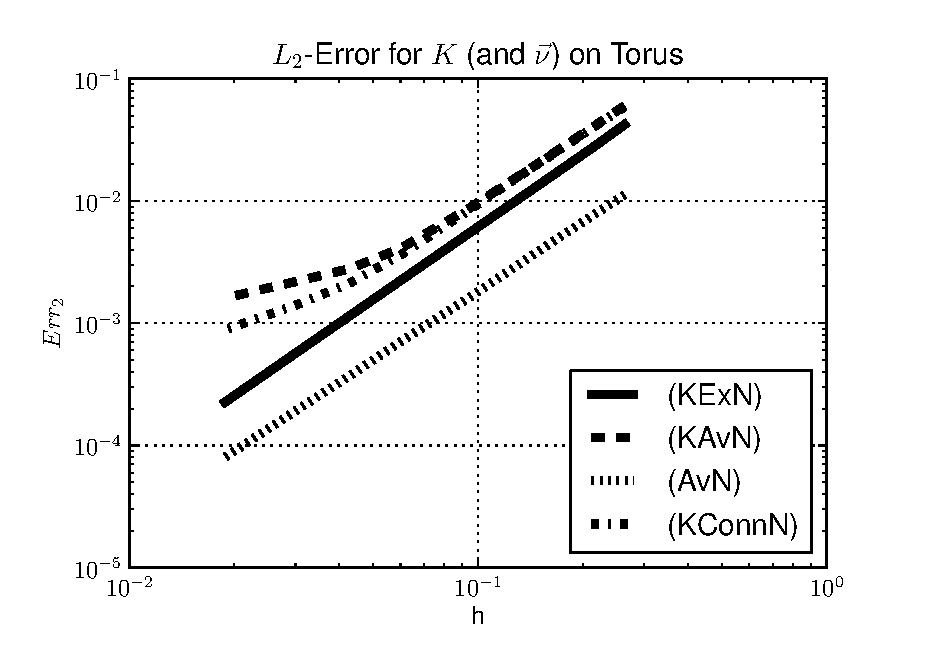
\includegraphics[width=\textwidth]{bilder/Curvature/TorusKWein2Plot.eps}
        \end{minipage} \hfill
        \begin{minipage}[t]{0.49\textwidth}
          \centering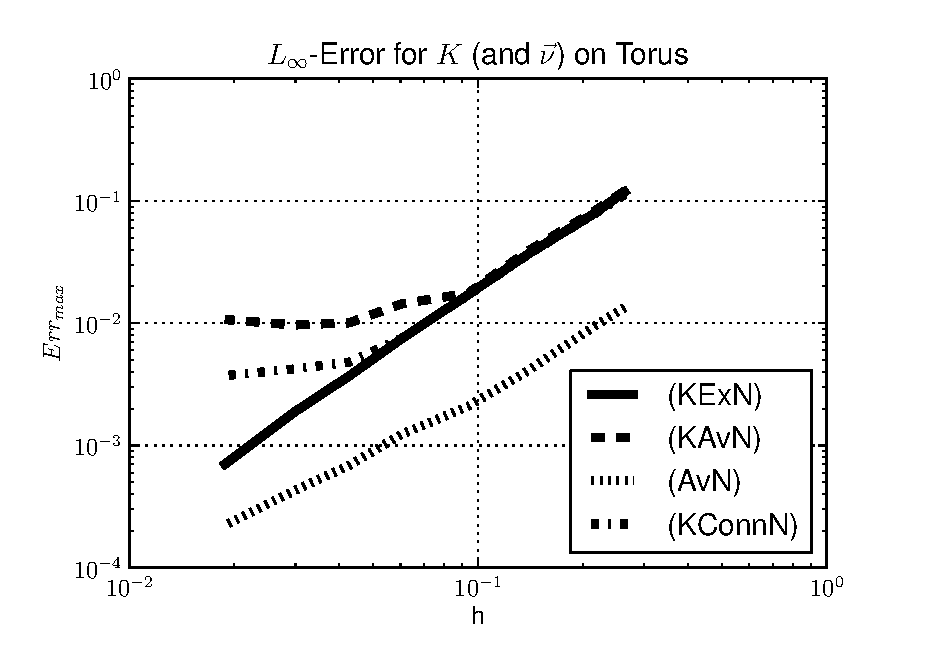
\includegraphics[width=\textwidth]{bilder/Curvature/TorusKWeinMaxPlot.eps}
        \end{minipage}\\
        \begin{minipage}[t]{0.49\textwidth}
          \centering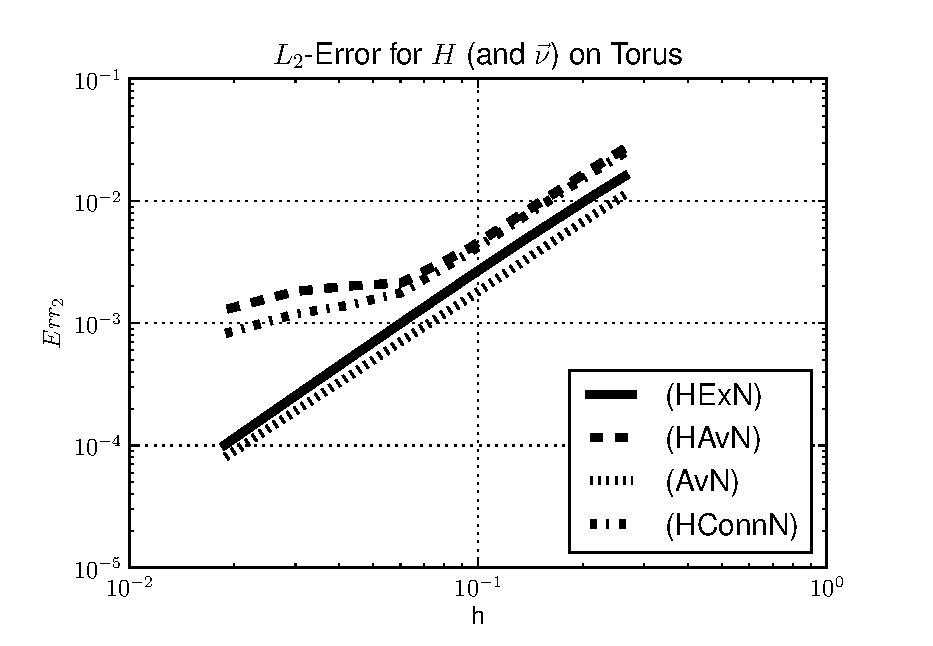
\includegraphics[width=\textwidth]{bilder/Curvature/TorusHWein2Plot.eps}
        \end{minipage}\hfill
        \begin{minipage}[t]{0.49\textwidth}
          \centering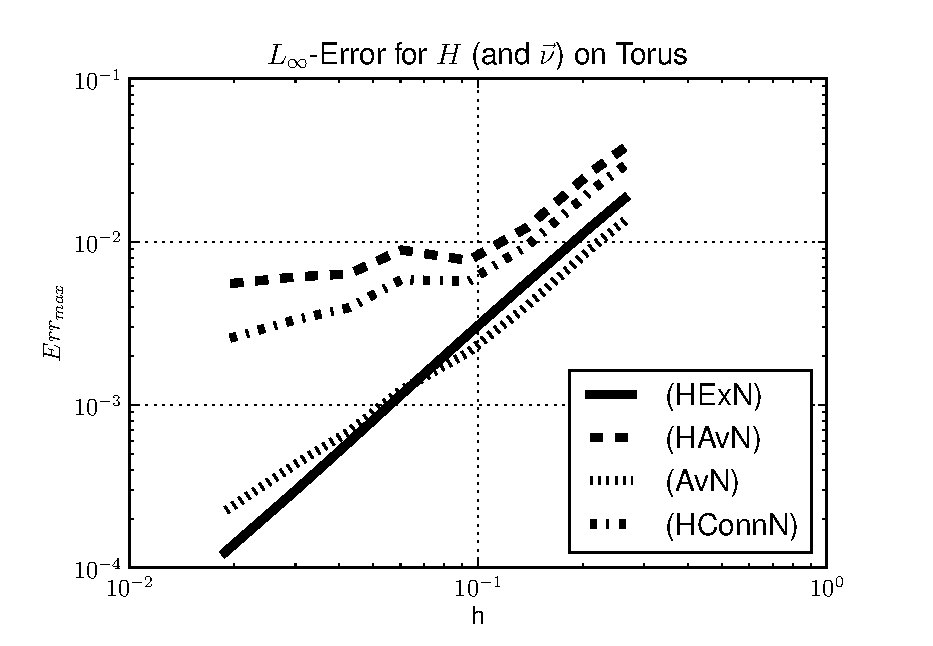
\includegraphics[width=\textwidth]{bilder/Curvature/TorusHWeinMaxPlot.eps}
        \end{minipage}
        \caption[Fehler Gauß-/mittlere Krümmung aus Weingartenabb. auf Torus]
                {(Log-Log-Plot) Fehler in diskreter \( L_{2} \)- und Maximumsnorm für die Gaußkrümmung \( K \) bzw. mittlere Krümmung \( H \) berechnet aus
                der Weingartenabbildung mit exakten Normalen (KExN)/(HExN), 
                nach \eqref{eqNormalMittel} gemittelte Elementnormalen (KAvN)/(HAvN) 
                und nach \eqref{eqNormalConnMittel} gemittelte Elementnormalen (KConnN)/(HConnN).
                Zudem ist auch der Fehler der Normalenmittelung nach \eqref{eqNormalMittel} in der jeweiligen Norm zu sehen (AvN).}
        \label{figWeingartenFehlerTorus}
      \end{figure}
    \end{beispiel}

    \begin{fazit}
      Wenn die Normalenvektoren an jedem Koten der Obeflächentriangulierung bekannt sind, zum Beispiel aus einer Parametrisierung
      \( \vec{x}: \left( u,v \right) \mapsto \left( x,y,z \right)\) durch
      \begin{align}
        \vec{\nu} &= \frac{\frac{\partial\vec{x}}{\partial u} \times \frac{\partial\vec{x}}{\partial v}}
                             {\left\| \frac{\partial\vec{x}}{\partial u} \times \frac{\partial\vec{x}}{\partial v} \right\|}
      \end{align}
      oder einer signierten Distanzfunktion \( \varphi \) durch
      \begin{align}
        \label{eqNormalsFromSignDist}
        \vec{\nu} &= \frac{\nabla_{\R^{3}}\varphi}{\left\| \nabla_{\R^{3}}\varphi \right\|} \formkomma
      \end{align}
      dann können mit der diskreten Weingartenabbildung gute Ergebnisse erzielt werden.
      Sind dagegen die Normalen nicht bekannt, so muss in zukünftigen Arbeiten eine angepasstere Möglichkeit bereitgestellt
      werden die Normalen an den Ecken des Polyeders zu gewinnen. 
      Oder es wird ein, für diese Problemstellung geeigneter, diskreter Gradient,
      zum Beispiel ein Dual-Primär-Gradient für eine diskrete duale \( 0 \)-Form ausgewertet auf den primären Gitterpunkten, entwickelt.
      Hätten wir so einen Gradienten, dann könnten wir die Elementnormalen \( \vecover{\nu}{\sigma^{2}} \) direkt 
      für eine
      Berechnung der diskreten Weingartenabbildung auf den Ecken auswerten.

      In Abschnitt \ref{secNumEx} wird zudem die hier vorgestellte Krümmungsapproximation auch auf anderen Oberflächen getestet und mit den
      Ergebnissen von \cite{heine} verglichen.
    \end{fazit}



\section{Krümmungsvektor}
  \label{secKruemmungsvektor}
  Der Krümmungsvektor \( \vec{H} \) ist die mittlere Krümmung in Normalenrichtung unter Beachtung der Dimension \( n \) der Oberfläche.
  Für eine \( 2 \)-Mannigfaltigkeit gilt
  \begin{align}
    \label{eqDefKruemmungsvektor}
    \vec{H} := 2 H \vec{\nu} \formpunkt
  \end{align}
  Nach \cite[4.5]{chen} bzw. \cite[4.5]{flanders} gilt für jede isometrische Immersion \( \vec{x}:M\rightarrow \R^{3} \)
  \begin{align}
    -\Delta_{B}\vec{x} = \vec{H} \formkomma
  \end{align}
  wobei auch hier wieder die Gleichung komponentenweise, also als vektorisiertes skalarwertiges Problem, zu sehen ist.
  Da wir numerisch nicht in lokalen Koordinaten rechnen möchten (außer zur Verifizierung der Ergebnisse) und uns die Oberfläche als
  Punktmenge im \( \R^{3} \) vorliegt, wählen wir als Abbildung zwischen der Oberfläche und dem \( \R^{3} \) einfach die Inklusion, das heißt
  \begin{align}
    \vec{x}:= \iota: \R^{3}\supset M \hookrightarrow \R^{3} \formpunkt
  \end{align}
  Es ist leicht zu sehen, dass die Inklusion als Identität eingeschränkt auf \( M \) eine isometrische Immersion ist 
  (\( g\equiv I \) und der Pushforward \( \iota_{*}:T_{p}M \hookrightarrow T_{p}\R^{3} \) ist injektiv).
  Mit Hilfe des DEC-diskretisierten Laplace-Beltrami-Operators erhalten wir nun das diskrete Problem
  \begin{align}
    \label{eqProbLX}
    \left\langle \vec{H}, v \right\rangle = - \left\langle \Delta_{B}\vec{x} , v \right\rangle
  \end{align}
  für alle Ecken \( v\in K^{(0)} \).
  Durch Anwenden des Hodge-Stern-Operators auf beiden Seiten können wir das resultierende "`duale"' Problem in gewohnter Weise in AMDiS
  lösen (vgl. Abschnitt \ref{subsecLaplaceImplementierung}).
  Als \( \R^{3} \)-vektorisierte Aufgabenstellung kann dabei auch jede der drei Komponenten unabhängig voneinander gelöst werden.
  Nach \eqref{eqDefKruemmungsvektor} lässt sich die mittlere Krümmung über die euklidische Norm des Krümmungsvektors erhalten, also
  \begin{align}
    H = \frac{1}{2}\left\| \vec{H} \right\|_{\R^{3}} \formpunkt
  \end{align}
  Numerische Beispiele dazu finden sich im Abschnitt \ref{secNumEx}.

\section{Gauß-Bonnet-Operator}
  Eine weitere Möglichkeit die Gaußsche Krümmung zu approximieren besteht aus einem einfachen geometrischen Ansatz, der aus dem Satz von
  Gauß-Bonnet folgt. 
  Dieser Satz besagt speziell für eine orientierte Riemannsche Mannigfaltigkeit \( P \) mit nur stückweise differenzierbaren Rand (vgl.
  \cite[Kap.10.5]{berger})
  \begin{align}
    \label{eqGaussBonnet}
    \int_{P}K \mu = 2\pi - \sum_{i=1}^{m}\beta_{i} - \int_{\partial P} k_{g} ds
  \end{align}
  wobei \( \beta_{i} \) die Außenwinkel an den \( m \) "`Knicken"' der Randkurve sind und \( k_{g} \) die geodätische Krümmung der
  Randkurve ist.
  Diese Formel können wir auch auf eine abstrakte Voronoi-Zelle \( P=\star\pi(v)\in C_{2}(\star L) \) für die Ecke \( v \in K^{(0)}=L^{(0)} \)
  anwenden. 
  Da die "`Knicke"' immer genau im Umkreismittelpunkt der Dreieckelemente um \( v \) sind, 
  ergibt sich \( m=m_{v} \), die Anzahl der \( 2 \)-Simplizes des 1-Ringes um \( v \).
  Die Approximation besteht nun darin \mbox{\( \star v \in C_{2}(\star K) \)} als Näherung für \( \star\pi(v) \) in Gleichung \eqref{eqGaussBonnet}
  zu verwenden.
  Da die Randkurve \( \partial(\star v) \) auf den differenzierbaren Teilstücken gerade ist, verschwindet dort die geodätische Krümmung.
  An den Schnitten mit den Primärkanten 
  \begin{align}
    \star\sigma^{1}\cap\sigma^{1} = c(\sigma^{1})\in \csd K 
  \end{align}
  ist die 
  geodetische Krümmung ebenfalls null,
  da dort die Randkurve einen Winkel von genau \( \pi \) auf dem Polytop \( |K| \) hat (vgl. \cite{polthier}).
  Weil nun die Volumenform 
  \begin{align}
    \mu = \sqrt{|g|} dx^{1} \wedge dx^{2}
  \end{align}
  nichts weiter als das Hodge-Stern-Duale der Eins ist, das heißt 
  \( \mu = *1 \) und damit \mbox{\(  K \mu = *K \)}, ergibt sich folgende approximative Aufgabenstellung
  \begin{align}
      \label{eqDualGaussBonnet}
      \left\langle *K , \star v \right\rangle &\approx 2\pi - \sum_{i=1}^{m_{v}}\beta_{i}
  \end{align}
  mit den Außenwinkeln an den Ecken von \( \star v \) (vgl. Abb. \ref{figGaussBonnetWinkel}).
  Damit haben wir schon eine "`duale"' DEC-Formulierung der rechten Seite zur elementweisen Assemblierung über
  \begin{align}
    \left\langle *K , \star v \right\rangle = \left| \star v \right|\left\langle K, v \right\rangle
                          = \sum_{\sigma^{2}\succ v} \left| \star v \cap \sigma^{2} \right| \left\langle K, v \right\rangle
  \end{align}
  automatisch erhalten mit dem Freiheitsgrad \( K \) am Knoten \( v \).
  Der zugehörige "`primäre"' Gauß-Bonnet-Operator definiert sich dementsprechend in DEC-Notation durch
  \begin{align}
    \left\langle K^{GB},v \right\rangle := \frac{1}{\left| \star v \right|} \left( 2\pi - \sum_{i=1}^{m_{v}}\beta_{i} \right) \formpunkt
  \end{align}
  Der obere Index \( GB \) kann auch weggelassen werden, wenn klar ist, dass es sich um den Gauß-Bonnet-Operator handelt.

  \subsection{Implementierung}
    Um auch die rechte Seite von \eqref{eqDualGaussBonnet} elementweise zu berechnen, müssen die Außenwinkel auf jedem Dreieck berechnet
    werden.
    \begin{figure}
      \begin{minipage}[t]{0.49\textwidth}
        \centering\usetikzlibrary{calc}
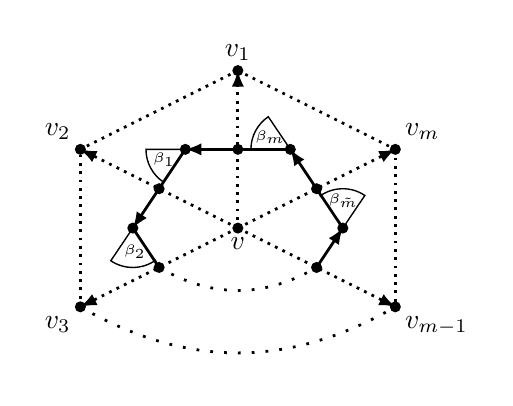
\begin{tikzpicture}[>=latex]
  % Coords
  \coordinate (V0) at (2,0);
  \coordinate (V1) at (2,2);
  \coordinate (V2) at (0,1);
  \coordinate (V3) at (4,1);
  \coordinate (V4) at (4,-1);
  \coordinate (V5) at (0,-1);
  % Arrows\tilde{\sigma}
  \draw[line width=1pt,style=dotted, ->]
    (V0) -- (V1);
  \draw[line width=1pt,style=dotted]
    (V1) --  (V2);
  \draw[line width=1pt,style=dotted, ->]
    (V0) -- (V2);
  \draw[line width=1pt,style=dotted]
    (V1) --  (V3);
  \draw[line width=1pt,style=dotted, ->]
    (V0) -- (V3);
   \draw[line width=1pt,style=dotted, ->]
    (V0) -- (V4);
  \draw[line width=1pt,style=dotted, ->]
    (V0) -- (V5);
  \draw[line width=1pt,style=dotted]
    (V5) --  (V2);
  \draw[line width=1pt,style=dotted]
    (V3) --  (V4);
  % Points
  \fill (V0) node[below] {\(v\)} circle (2pt);
  \fill (V1) node[above] {\(v_1\)} circle (2pt);
  \fill (V2) node[above left] {\(v_2\)} circle (2pt);
  \fill (V3) node[above right] {\(v_{m}\)} circle (2pt);
  \fill (V4) node[below right] {\(v_{m-1}\)} circle (2pt);
  \fill (V5) node[below left] {\(v_3\)} circle (2pt);
  \draw[line width=1pt, style=loosely dotted]
     (V5) to[bend right] (V4);
  %circumcenter
  \coordinate (CC1) at (1.333,1);
  \coordinate (CC0) at (2.666,1);
  \coordinate (CC2) at (0.666,0);
  \coordinate (CCm) at (3.333,0);
  \coordinate (CCC0) at (2,1);
  \coordinate (CCC1) at (1,0.5);
  \coordinate (CCC2) at (3,0.5);
  \coordinate (CCC3) at (1,-0.5);
  \coordinate (CCC4) at (3,-0.5);
  \fill (CC0) circle (2pt);
  \fill (CC1) circle (2pt);
  \fill (CC2) circle (2pt);
  \fill (CCm) circle (2pt);
  \fill (CCC0) circle (2pt);
  \fill (CCC1) circle (2pt);
  \fill (CCC2) circle (2pt);
  \fill (CCC3) circle (2pt);
  \fill (CCC4) circle (2pt);
  \draw[line width=1pt, ->] (CC0) -- (CC1);
  \draw[line width=1pt, ->] (CC1) -- (CC2);
  \draw[line width=1pt, ->] (CCm) -- (CC0);
  \draw[line width=1pt] (CC2) -- (CCC3);
  \draw[line width=1pt,->] (CCC4) -- (CCm);
  \draw[line width=1pt, style=loosely dotted]
     (CCC3) to[bend right] (CCC4);

%winkel
\draw[line width=0.5pt] (CC1) -- +(180:0.5) arc (180:236:0.5);
\node at ($(CC1)+(205:0.3)$) {\tiny\(\beta_1\)};
\draw[line width=0.5pt] (CC2) -- +(236:0.5) arc (236:306:0.5);
\node at ($(CC2)+(275:0.3)$) {\tiny\(\beta_2\)};
\draw[line width=0.5pt] (CC0) -- +(124:0.5) arc (124:180:0.5);
\node at ($(CC0)+(149:0.3)$) {\tiny\(\beta_m\)};
\draw[line width=0.5pt] (CCm) -- +(56:0.5) arc (56:126:0.5);
\node at ($(CCm)+(89:0.35)$) {\tiny\(\beta_{\tilde{m}}\)};
%\draw[line width=0.5pt] (V3) -- +(206.565:0.95) arc (206.565:153.435:0.95);
%\node[left] at (V3) {\(\beta_{0m}\ \)}; 
%\draw[line width=0.5pt] (V2) -- +(-26.565:0.9) arc (-26.565:26.565:0.9);
%\node[right] at (V2) {\(\ \alpha_{01}\)}; 


\useasboundingbox ([shift={(1mm,1mm)}]current bounding box.north east) rectangle ([shift={(-1mm,-1mm)}]current bounding box.south west);
\end{tikzpicture}


      \end{minipage}
      \hfill
      \begin{minipage}[t]{0.49\textwidth}
        \centering\usetikzlibrary{calc}
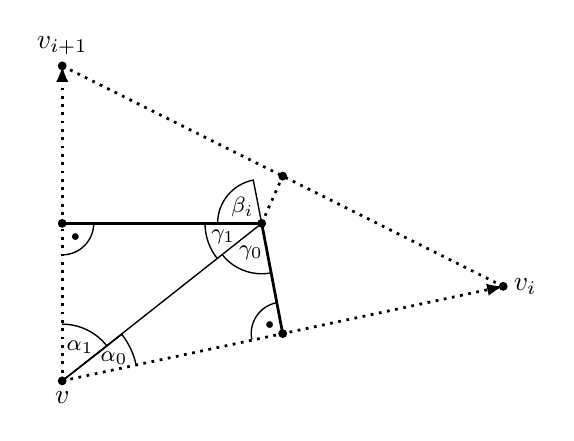
\begin{tikzpicture}[>=latex, line width=1pt, scale=0.8]
%coords
%center
\coordinate (C) at (3.1666,2.5);
%vertices
\coordinate (V) at (0,0);
\coordinate (Vi) at (7,1.5);
\coordinate (Vi1) at (0,5);
%edge centers
\coordinate (CCi) at (3.5,0.75);
\coordinate (CCi1) at (0,2.5);
\coordinate (CCii1) at (3.5,3.25);

%nodes
\fill (V) node[below] {\(v\)} circle(2pt);
\fill (Vi) node[right] {\(v_i\)} circle(2pt);
\fill (Vi1) node[above] {\(v_{i+1}\)} circle(2pt);
\fill (C) circle(2pt);
\fill (CCi) circle(2pt);
\fill (CCi1) circle(2pt);
\fill (CCii1) circle(2pt);

%lines
%edges
\draw[style=dotted, ->] (V) -- (Vi);
\draw[style=dotted] (Vi) -- (Vi1);
\draw[style=dotted, ->] (V) -- (Vi1);
%voronoi edges
\draw (CCi) -- (C);
\draw (C) -- (CCi1);
\draw[style=dotted] (C) -- (CCii1);
%nonelementary dual edge 
\draw[line width=0.5pt] (C) -- (V);

%angles
%rightangles
\draw[line width=0.5pt] (CCi) -- +(101:0.5) arc (101:191:0.5);
\node at ($(CCi)+(146:0.25)$) {\tiny\(\bullet\)};
\draw[line width=0.5pt] (CCi1) -- +(0:0.5) arc (0:-90:0.5);
\node at ($(CCi1)+(315:0.3)$) {\tiny\(\bullet\)};
%beta
\draw[line width=0.5pt] (C) -- +(101:0.7) arc (101:180:0.7);
\node at ($(C)+(140:0.4)$) {\footnotesize\(\beta_i\)};
%gammas
\draw[line width=0.5pt] (C) -- +(180:0.9) arc (180:219:0.9);
\node at ($(C)+(199.5:0.65)$) {\footnotesize\(\gamma_1\)};
\draw[line width=0.5pt] (C) -- +(281:0.8) arc (281:219:0.8);
\node at ($(C)+(250:0.5)$) {\footnotesize\(\gamma_0\)};
%alphas
\draw[line width=0.5pt] (V) -- +(38:0.9) arc (38:90:0.9);
\node at ($(V)+(62:0.6)$) {\footnotesize\(\alpha_1\)};
\draw[line width=0.5pt] (V) -- +(38:1.2) arc (38:12:1.2);
\node at ($(V)+(24:0.9)$) {\footnotesize\(\alpha_0\)};

\end{tikzpicture}
      \end{minipage}
      \caption[Außenwinkel der Voronoi-Zelle]{Die \( m = m_{v} =: \tilde{m}+1 \) Außenwinkel \( \beta_{i} \) an den Ecken der
                                             Voronoi-Zelle (links) 
                                             und die zugehörigen Innenwinkel bzgl. der Primär- und Dualkanten für ein Dreieckelement 
                                             \( \sigma^{2} \) (rechts).}
      \label{figGaussBonnetWinkel}
    \end{figure}
    Nun ist der Außenwinkel \( \beta_{i} \) gleich dem Innenwinkel des \( i \)-ten Dreiecks an der Ecke \( v \), denn mit den Bezeichnern
    aus Abbildung \ref{figGaussBonnetWinkel} gilt
    \begin{align}
      \gamma_{k} &= \frac{\pi}{2} - \alpha_{k} \quad (k = 0,1) \\
      \beta_{i} &= \pi - \gamma_{0} - \gamma_{1}
                 = \pi + \alpha_{0} - \frac{\pi}{2} + \alpha_{1} - \frac{\pi}{2} \\
                &= \alpha_{0} + \alpha_{1} \formpunkt
    \end{align}
    Weiterhin lassen sich die Winkel \( \alpha_{k} \) über die Längen der Primärkanten und der auf
    \mbox{\( \sigma^{2}=\left[ v, v_{i}, v_{i+1} \right] \)} eingeschränkten Voronoi-Kanten bestimmen durch
    \begin{align}
      \alpha_{k} &= \arctan\left( \frac{\left|\star\left[ v, v_{i+k} \right] \cap \sigma^{2} \right|}
                                    {\frac{1}{2}\left|\left[ v, v_{i+k} \right]\right|} \right)
                  = \text{atan2}\left( 2\left|\star\left[ v, v_{i+k} \right] \cap \sigma^{2} \right|, 
                                 \left|\left[ v, v_{i+k} \right]\right|\right) \formpunkt
    \end{align}
    Insgesamt erhalten wir also für die Summe der Außenwinkel der Voronoi-Zelle \( \star v \)
    \begin{align}
      \label{eqAussenwinkelsummeAtan}
      \sum_{i=1}^{m_{v}}\beta_{i} &= \sum_{\sigma^{2}\succ v} \sum_{\sigma^{2}\succ\sigma^{1}\succ v}
                               \text{atan2}\left( 2\left|\star\sigma^{1} \cap \sigma^{2} \right|, 
                                 \left|\sigma^{1}\right|\right) \formkomma       
    \end{align}
    die somit immer noch elementweise bestimmt werden kann.
    Ein Problem stellt jedoch noch der Minuend \( 2\pi \) in der rechten Seite von \ref{eqDualGaussBonnet} dar.
    Eine Möglichkeit wäre es, den globalen Rechte-Seite-Vektor mit \( \left[ 2\pi \right]_{v\in K^{(0)}} \), statt wie
    gewohnt mit \( \left[ 0 \right]_{v\in K^{(0)}} \), zu initialisieren und beim Assemblieren die sich aus 
    \eqref{eqAussenwinkelsummeAtan} ergebenden Elementvektoren abzuziehen.
    Eine andere Möglichkeit ist es \( 2\pi \) selbst auch elementweise zu zerlegen, sodass wir
    \begin{align}
      \label{eqProbGB}
      \left\langle *K^{GB} , \star v \right\rangle &=
      2\pi - \sum_{i=1}^{m_{v}}\beta_{i} =
          \sum_{\sigma^{2}\succ v} \left( \frac{2\pi}{m_{v}} - \sum_{\sigma^{2}\succ\sigma^{1}\succ v}
                               \text{atan2}\left( 2\left|\star\sigma^{1} \cap \sigma^{2} \right|, 
                                 \left|\sigma^{1}\right|\right) \right)
    \end{align}
    für die Voronoi-Zelle am Knoten \( v \) erhalten. 
    Jedoch ist zu bedenken, dass \( m_{v} \) a priori auf einem Dreieckelement nicht bekannt ist.
    Somit wäre es sinnvoll \( m_{v} \) für alle Ecken \( v\in K^{(0)} \) noch vor dem Aufstellen der Systemmatrix zu bestimmen falls eine
    Parallelisierung des Assemblierungsalgorithmus gewünscht ist.

    Ein Algorithmus zur Berechnung der Elementvektoren ist im Appendix \ref{subsecAlgoGaussBonnet} gegeben.
    In Abschnitt \ref{secNumEx} werden wir den Operator als Vergleich zur diskreten Weingartenabbildung und den Ergebnissen von \cite{heine} testen. 
    In \cite{meyer} wird der Gauß-Bonnet-Operator ebenfalls mit anderen Methoden verglichen.

\section{Numerisches Experiment}
\label{secNumEx}
  
  Zur Bestimmung der Gaußkrümmung \( K \) und der mittleren Krümmung \( H \) stehen uns nun jeweils drei Methoden zur Verfügung.
  Die Gaußsche Krümmung kann aus der diskreten Weingartenabbildung mit (SK) und ohne (SKAvN) gegebenem Normalenfeld 
  oder mit Hilfe des Gauß-Bonnet-Operators (GB) berechnet werden.
  Die mittlere Krümmung kann ebenfalls aus der diskreten Weingartenabbildung (SH/SHAvN) oder aus dem Krüm"-mungs"-vektor, der aus dem diskreten Laplace-Beltrami-Operators der Koordinatenabbildung
  folgt (LX), berechnet werden.

  In \cite{heine} wird \( K \) und \( H \) auch aus einer Approximation der Weingartenabbildung gewonnen.
  Hierbei wird ein isoparametrischer Finite-Elemente-Ansatz (FEM) genutzt. 
  Die Oberfläche \( M \) wird elementweise Lagrange-interpoliert zu \( M^{\gamma}_{h} \) mit dem Polynomgrad \( \gamma\in\left\{ 1,2,3,4 \right\} \).
  Zunächst wird dabei \( M \) linear zu \(\mathcal{T}^{1}_{h}  \) trianguliert, sodass
  \begin{align}
     M_{h}^{1} = |K|  \formtext{und}
     \mathcal{T}^{1}_{h} = K^{(2)}
  \end{align}
  gilt.
  Für \( \gamma = 2,3,4 \) werden dann die noch übrigen \( 3 \), \( 7 \) bzw. \( 12 \) Lagrange-Knoten \( Q_{i}\in\sigma^{2} \) durch \( \pi\left( Q_{i} \right)\in M \) orthogonal projiziert.
  Der Raum der Ansatzfunktion definiert sich dann über
  \begin{align}
    W_{h}^{\gamma} 
      &:= \left\{ w_{h}\in C^{0,1}\left( M_{h}^{\gamma} \right) \middle|\  
                          \forall T_{h}^{\gamma} \in \mathcal{T}_{h}^{\gamma}:\  \left( w_{h} \circ \Phi_{T_{h}^{1}}^{\gamma}\right) \in \mathds{P}_{\gamma}\left(\hat{T}\right)\right\}
                          \formkomma
  \end{align}
  wobei \( \hat{T}:=\Delta^{2}\in\R^{2} \) das Referenzdreieck ist und 
  \( \Phi_{T_{h}^{1}}^{\gamma}: \hat{T} \rightarrow T_{h}^{1} \)
  die polynomiale Parametrisierung vom Grad \( \gamma \).
  Das diskrete Problem für die Weingartenabbildung lautete nun für alle \( \vec{\psi}_{h}\in \left( W_{h}^{\gamma} \right)^{3} \)
  und \( j\in\left\{ 1,2,3 \right\} \)
  \begin{align}
    \int_{M_{h}^{\gamma}} \II_{h}^{j} \cdot \vec{\psi}_{h} \mu
        &= -\int_{M_{h}^{\gamma}} \nu_{h}^{j} \left( \nabla_{M_{h}^{\gamma}} \cdot \vec{\psi}_{h} + \vec{H}_{h}\cdot\vec{\psi}_{h} \right) \mu
  \end{align}
  mit der diskreten Weingartenabbildung 
  \begin{align}
    \II_{h} = \left[ \II_{h}^{1}, \II_{h}^{2}, \II_{h}^{3} \right] \in \left( W_{h}^{\gamma} \right)^{3 \times 3}
  \end{align}
  als Lösung.
  \( \vec{\nu}_{h}=\left[ \nu_{h}^{1}, \nu_{h}^{2}, \nu_{h}^{3} \right]^{T} \) ist das äußere Normalenfeld von \( M_{h}^{\gamma} \).
  Des Weiteren ist die Tangentialdivergenz der vektorisierten Ansatzfunktion \( \vec{\psi}_{h} = \left[ \psi_{h}^{1}, \psi_{h}^{2}, \psi_{h}^{3} \right]^{T} \) definiert als
  \begin{align}
    \nabla_{M_{h}^{\gamma}} \cdot \vec{\psi}_{h} := \nabla_{\R^{3}} \cdot \vec{\psi}_{h} 
                          - \sum_{i=1}^{3 }\left( \nabla_{\R^{3}}\psi_{h}^{i} \cdot \vec{\nu}_{h} \right) \nu_{h}^{i} \formpunkt
  \end{align}
  Der diskrete Krümmungsvektor \( \vec{H}_{h} := \left[ H_{h}^{1}, H_{h}^{2}, H_{h}^{3} \right]^{T} \in\left( W_{h}^{\gamma} \right)^{3} \) ergibt sich als Lösung von
  \begin{align}
    \int_{M_{h}^{\gamma}} H_{h}^{i} \psi_{h}^{i} \mu
      &=  \int_{M_{h}^{\gamma}} \nabla_{M_{h}^{\gamma}} x_{h}^{i} \cdot \nabla_{M_{h}^{\gamma}}\psi_{h}^{i} \mu
  \end{align}
  für alle \( i\in\left\{ 1,2,3 \right\} \) und \( \vec{\psi}_{h}\in \left( W_{h}^{\gamma} \right)^{3} \).
  Dabei ist \( \vec{x}_{h} = \left[ x_{h}^{1}, x_{h}^{2}, x_{h}^{3}\right]^{T} \) die Identität 
  und \mbox{\(\nabla_{M_{h}^{\gamma}} = \left( I - \vec{\nu}_{h} \vec{\nu}^{T}_{h} \right)\nabla_{\R^{3}} \)} der Oberflächengradient auf \( M_{h}^{\gamma} \). 
  Weitere Einzelheiten dazu kön"-nen in \cite{heine} nachgelesen werden.
  
  Als Oberflächen wählen wir drei, welche auch in \cite{heine} genutzt werden. 
  Dazu gehören die Einheitssphäre (Appendix \ref{sphere}), eine quartische Oberfläche, die sich als Null-Level-Sets eines Polynomes vierten
  Grades beschreiben lässt (Appendix \ref{heineB}) und ein Ellipsoid (Appendix \ref{heineC}).
  Für unsere Berechnungen, wie auch bei \cite{heine}, ist die Makrotriangulation ein Ikosaeder projiziert auf die Oberfläche.
  Da für die DEC-Diskretisierung Wohlzentriertheit an das Primärgitter gestellt wird, verfeinern wir zunächst die Ikosaederflächen.
  Für die Sphäre ist bei dem hier verwendeten Verfeinerungsmechanismus \mbox{(Cinema4D)} nichts weiter zu tun, da wir schon eine sehr gleichmäßige
  Triangulierung erhalten.
  Für die anderen beiden Oberflächen verwenden wir den in Abschnitt \ref{secGittergenerierung} vorgestellten Algorithmus um die
  Triangulierung zu verbessern und Wohlzentriertheit zu gewährleisten.
  Ein Nachteil dieser Prozedur ist, dass gerade an Orten mit starker Krümmung das Gitter schlechter aufgelöst wird als bei flacheren
  Umgebungen. 
  So war es zum Beispiel nicht möglich, für gröbere Gitter unter ca. 5300 Gitterpunkten (\( h\approx 0.26 \)), bei der quartischen
  Oberfläche, die beiden Wölbungen ordentlich darzustellen, wie wir in Abbildung \ref{figHeineBResolution} sehen können.
  
  Die exakten mittleren Krümmungen und die Gaußschen Krümmungen für den Ellipsoiden und der quartischen Oberfläche
  sind in Abbildung \ref{figErrCurvHeineB} bzw. \ref{figErrCurvHeineC} dargestellt.
  Für die Sphäre sind beide Krümmungsgrößen konstant eins.

  Für die Berechnung der Weingartenabbildung werden zum einen die gemittelten Normalen verwendet (S*AvN), das heißt es werden die
  Gleichungen \eqref{eqWeingartenEq1}+\eqref{eqWeingartenEq2} gelöst 
  (\( 3 \cdot (9+3) = 36 \) DOFs p. Element\footnote{lokale Freiheitsgrade}).
  Zum anderem nutzen wir die exakten Normalen (S*) an den Knoten, die wir durch die genormten Gradienten der
  signierten Distanzfunktion erhalten (vgl. \eqref{eqNormalsFromSignDist})
  und lösen nur Gleichung \eqref{eqWeingartenEq2} (\( 3 \cdot 9 = 27 \) DOFs p. Element).
  Zum Vergleich, bei \cite{heine} müssen zu den 9 Komponenten der Weingartenabbildung auch noch die 3 Komponenten des Krümmungsvektors
  berechnet werden, das heißt für die linearen Elemente sind ebenfalls \( 3 \cdot (9+3) = 36 \) DOFs pro Element zu bestimmen, wie auch bei
  unserem (S*AvN)-Problem. 
  Für den Grad 2, 3 bzw. 4 sind es dann schon \( 72 \), \( 120 \) bzw. \( 180 \) DOFs pro Element.
  Für unsere Berechnung der mittleren Krümmung direkt aus dem Krümmungsvektor (LX) nach Gleichung
  \eqref{eqProbLX} erhalten wir nur \( 9 \) DOFs pro Element
  und für die Ermittlung der Gaußkrümmung mit dem Gauß-Bonnet-Operator nach Gleichung \eqref{eqProbGB}
  sogar nur \( 3 \) DOFs pro Dreieckelement.
  Prinzipiell sollte sich der Assemblierungsaufwand für einen einzelnen Freiheitsgrad asymptotisch nich von
  der FEM-Diskretisierung unterscheiden,
  da bei der FEM-Diskretisierung mit den Gittern in \cite{heine} im Mittel etwa genauso viele Elemente 
  (ca. 6) für die Assemblierung eines globalen DOFs beteiligt sind.
  Bei allen Problemen ließe sich im "`Primärraum"' auf das Lösen eines linearen Gleichungssystem verzichten, 
  da sich auch bei den 
  (S*AvN)-Problemen die Gleichungen entkoppeln lassen, sodass alle zu berechnenden Größen auf
  der rechten Seite stehen (Vektoroperatoren) und auf der linken Seite nur die Identität als Systemmatrix.
  Da wir uns aber wegen dem Vorteil der einfacheren elementweisen Assemblierung dazu entschlossen hatten im
  "`Dualraum"' zu rechnen, haben wir für die entkoppelten Probleme einen Eintrag pro Zeile in der
  Systemmatrix, der den metrischen Faktor \( \left| \star v \right| \) für jeden Knoten \( v\in K^{(0)} \)
  enthält. 
  Um auch zu zeigen, dass Differentialgleichungssysteme mit einem DEC möglich sind, lösen wir die
  (S*AvN)-Probleme (\eqref{eqWeingartenEq1}+\eqref{eqWeingartenEq2}) nicht entkoppelt, sodass in der
  Systemmatrix, wegen der impliziten Berechnung der Normalen-Gradienten, 7 Nicht-Null-Einträge für Knoten
  mit hexagonaler Struktur und 6 für die Defekte (Fünfer-1-Ring) pro Zeile stehen.
  Da in \cite{heine} keine genaue Aussage getroffen wird, wie hoch der tatsächlich betriebene relative Aufwand ist,
  können wir davon ausgehen, dass die Anzahl der Freiheitsgrade ein geeignetes Maß dafür ist.
  Somit sind die Kosten für alle hier vorgestellten DEC-Probleme kleiner oder gleich (für (S*AvN)) dem der
  isoparametrischen FEM vom Grade 1.
  Für das Lösen der dünnbesetzten Gleichungssysteme wird in allen Fällen einheitlich der
  BiCGStab2-Algorithmus mit einer Abbruchstoleranz von \( 1.0E-10 \) benutzt.
  Wie zu erwarten, übersteigt der Assemblierungsaufwand in den meisten Fällen den des Lösungsaufwandes.

  In den Tabellen \ref{tabSphereWeingarten} - \ref{tabHeineCGBLX} sind die relativen Fehler 
  und die sich ergebenden experimentellen Konvergenzordnungen der sechs
  DEC-Probleme (SK, SH, SKAvN, SHAvN, GB, LX) zu unterschiedlichen maximalen Gitterweiten niedergeschrieben.
  Tabellarische Ergebnisse der gleichen Form für die isoparametrische FEM können in \cite{heine} nachgelesen werden.
  In den Abbildungen \ref{figErrCompSphere}, \ref{figErrCompHeineB} und \ref{figErrCompHeineC} sind die
  relativen FEM-Fehler als Vergleich mitgezeichnet worden.
  Dabei sei zu bemerken das der lineare FE-Ansatz gar nicht konvergierte.

  Für (SK) und (SH) sind die Ergebnisse für die Sphäre und den Ellipsoiden mit denen der FEM vom Grad 2 und
  3 in etwa vergleichbar. 
  Dagegen fällt das Konvergenzverhalten auf der quartischen Oberfläche nicht so gut aus.
  Jedoch liegt die Vermutung nahe, dass die Konvergenzordnung mit feiner werdendem Gitter, unter
  Vernachlässigung von Rundungsfehlern, noch steigt, wie
  wir das zum Beispiel auch auf dem Ellipsoiden sehen können.
  Die größten Fehler kommen erwartungsgemäß dort vor, wo die Krümmung am größten ist, wie wir in Abbildung
  \ref{figErrCurvHeineB} für den Ellipsoiden und \ref{figErrCurvHeineC} für die quartische Oberfläche sehen
  können.
  Das liegt vermutlich zum größten Teil an der wesentlich schlechteren Gitterauflösung an diesen Stellen.
  Für den Fall, dass die Normalen weder explizit noch implizit an den Gitterknoten bekannt wären, stehen
  die Problemformulierungen (SKAvN) und (SHAvN) zur Verfügung.
  Dabei fallen die Konvergenztests schlechter aus als bei den (S*)-Problemen.
  Vor allem in der Maximumsnorm bricht in den meisten Fällen die Konvergenzrate ab einer bestimmten
  Gitterweite ein.
  Dieses Verhalten war schon auf dem Torus im Beispiel \ref{bspWeinTorus} zu beobachten.
  
  Das Verhalten der Fehler der Gaußschen Krümmung mit dem Gauß-Bonnet-Operator (GB) überrascht ein wenig.
  Wie wir sehen, konnten solide Ergebnisse erzielt werden trotz des sehr geringen Aufwandes für die Berechnung.
  Einzig in der Maximumsnorm auf dem Ellipsoiden war keine Konvergenz messbar.
  Hier hält sich vor allem der Fehler an den seitlichen Defekten hartnäckig (vgl. Abb.
  \ref{figErrCurvHeineC}).

  Das (LX)-Problem zur Berechnung der mittleren Krümmung brachte auf der Sphäre im Vergleich zu allen
  anderen Verfahren die besten Ergebnisse hervor. 
  Der Grund für das Abnehmen der experimentellen Konvergenzordnung ist die Genauigkeit der Lösung des
  linearen Gleichungssystems.
  Mit einer kleineren Abbruchstoleranz für den BiCGStab2 ließe sich auch eine Konvergenzrate von über 3
  beibehalten.
  Auf der quartischen Oberfläche stagniert vor allem die Konvergenzrate in der \( L_{2} \)-Norm, wobei sie
  in der Maximumsnorm etwa linear bleibt. 
  Das lässt darauf schließen, dass die größeren Fehler sich in einem festen Bereich der Oberfläche
  befinden.
  Wie wir in Abbildung \ref{figErrCurvHeineB} sehen können, sind die Fehler im Bereich der Sattelfläche
  recht hoch, obwohl dort das Gitter vergleichsweise fein ist.
  Auf einer Sattelfläche ist die eine Hauptkrümmung negativ und die andere positiv. 
  Folglich ist die
  Gaußsche Krümmung dort negativ. 
  Solch eine Situation liegt auch im "`inneren Bereich"' des Torus vor und auch hier haben wir ein ähnliches
  Fehlerverhalten, wie eine Vergleichsrechnung zeigt (siehe Abb. \ref{figLXDiameterTorus}).
  Während auf dem Ellipsoiden die Konvergenzrate in der diskreten \( L_{2} \)-Norm etwas unter 2 bleibt,
  bricht sie in der Maximumsnorm ein.
  Die maximalen Fehler befinden sich dort, wo die Krümmung am stärksten ist und zudem die
  Gitterauflösung vergleichsweise schlecht (vgl. \ref{figErrCurvHeineC}).

  Insgesamt schneiden alle DEC-Diskretisierungen im Vergleich zu den FEM"=Diskretisierungen in Hinblick auf den Aufwand ganz gut ab.
  Denn unter der Annahme, dass bei beiden Ansätzen ähnlich gleichmäßige Gitter verwendet werden, lohnt sich ein Blick auf die zum Teil stark unterschiedlichen Anzahlen der Freiheitsgrade
  pro Element, wie wir in Tabelle \ref{tabDOFsVergleich} sehen können. 

  \begin{table}[htbp]
    \centering
    \begin{tabular}{|r|r|r|r|r|r|}
      \hline
       & lDOFs & FEM 1 & FEM 2 & FEM 3 & FEM 4 \\\hline
       lDOFs & & 36 & 72 & 120 & 180 \\\hline
       (S*AvN) & 36 & 100\% & 50\%   & 30\%   & 20\%  \\\hline
       (S*)    & 27 & 75\%  & 37.5\% & 22.5\% & 15\% \\\hline
       (LX)    & 9  & 25\%  & 12.5\% & 7.5\%  & 5\% \\\hline
       (GB)    & 3  & 8.33\% & 4.17\% & 2.5\% & 1.67\% \\\hline
    \end{tabular}
    \caption[lDOFs Vergleich]{Verhältnis der Anzahl der lokalen Freiheitsgrade (lDOFs, DOFs pro Element) zwischen den DEC-Methoden und FEM.
                              FEM \( i \) bezeichnet hierbei die isoparametrische FEM mit \( \gamma = i \).}
    \label{tabDOFsVergleich}
  \end{table}
  
   \begin{table}[htbp]
    \centering
      \begin{tabular}{|l|r|r|r|r|r|r|r|r|}
      \hline
      \multicolumn{1}{|c|}{\rule{0pt}{11pt}\( h \)} & \multicolumn{1}{c|}{\( \err_{2}^{SK} \)} & \multicolumn{1}{c|}{EOC} & 
           \multicolumn{1}{c|}{\( \err_{\infty}^{SK} \)} & \multicolumn{1}{c|}{EOC} & \multicolumn{1}{c|}{\( \err_{2}^{SH} \)} &
           \multicolumn{1}{c|}{EOC} & \multicolumn{1}{c|}{\( \err_{\infty}^{SH} \)} & \multicolumn{1}{c|}{EOC} \\ \hline
      0.152 & 4.93E-03 & \multicolumn{1}{l|}{} & 5.69E-03 & \multicolumn{1}{l|}{} & 2.47E-03 & \multicolumn{1}{l|}{} & 2.85E-03 & \multicolumn{1}{l|}{} \\ \hline
      0.109 & 2.53E-03 & 2.00 & 2.94E-03 & 1.97 & 1.26E-03 & 2.00 & 1.47E-03 & 1.98 \\ \hline
      0.0664 & 9.39E-04 & 2.00 & 1.10E-03 & 1.99 & 4.70E-04 & 2.00 & 5.49E-04 & 1.99 \\ \hline
      0.0477 & 4.85E-04 & 2.00 & 5.69E-04 & 1.99 & 2.43E-04 & 2.00 & 2.84E-04 & 2.00 \\ \hline
      0.0306 & 1.99E-04 & 2.00 & 2.33E-04 & 2.00 & 9.95E-05 & 2.00 & 1.17E-04 & 2.00 \\ \hline
      0.0215 & 9.87E-05 & 2.00 & 1.16E-04 & 2.00 & 4.93E-05 & 2.00 & 5.79E-05 & 2.00 \\ \hline
      0.0153 & 4.98E-05 & 2.00 & 5.83E-05 & 2.00 & 2.49E-05 & 2.00 & 2.92E-05 & 2.00 \\ \hline
      0.00967 & 1.99E-05 & 2.00 & 2.34E-05 & 2.00 & 9.97E-06 & 2.00 & 1.17E-05 & 2.00 \\ \hline
      \end{tabular}
      \caption[Weingarten auf der Sphäre (S*)]{Relative Fehler für \( K \) und \( H \) (diskrete Weingartenabbildung(S*)) auf der Sphäre.}
      \label{tabSphereWeingarten}
      \vspace{10pt}
    \centering
      \begin{tabular}{|l|r|r|r|r|r|r|r|r|}
      \hline
      \multicolumn{1}{|c|}{\rule{0pt}{11pt}\( h \)} & \multicolumn{1}{c|}{\( \err_{2}^{SK} \)} & \multicolumn{1}{c|}{EOC} & 
           \multicolumn{1}{c|}{\( \err_{\infty}^{SK} \)} & \multicolumn{1}{c|}{EOC} & \multicolumn{1}{c|}{\( \err_{2}^{SH} \)} &
           \multicolumn{1}{c|}{EOC} & \multicolumn{1}{c|}{\( \err_{\infty}^{SH} \)} & \multicolumn{1}{c|}{EOC} \\ \hline
           0.152 & 2.63E-02 & \multicolumn{1}{l|}{} & 5.22E-02 & \multicolumn{1}{l|}{} & 1.32E-02 & \multicolumn{1}{l|}{} & 2.58E-02 & \multicolumn{1}{l|}{} \\ \hline
            0.109 & 1.65E-02 & 1.38 & 3.35E-02 & 1.32 & 8.31E-03 & 1.39 & 1.66E-02 & 1.31 \\ \hline
            0.0664 & 8.09E-03 & 1.44 & 1.81E-02 & 1.24 & 4.06E-03 & 1.45 & 9.07E-03 & 1.22 \\ \hline
            0.0477 & 4.99E-03 & 1.47 & 1.45E-02 & 0.68 & 2.50E-03 & 1.47 & 7.25E-03 & 0.68 \\ \hline
            0.0306 & 2.59E-03 & 1.47 & 2.31E-02 & -1.05 & 1.30E-03 & 1.47 & 1.16E-02 & -1.06 \\ \hline
            0.0215 & 1.56E-03 & 1.45 & 2.95E-02 & -0.69 & 7.79E-04 & 1.45 & 1.48E-02 & -0.70 \\ \hline
            0.0153 & 9.52E-04 & 1.44 & 3.38E-02 & -0.40 & 4.77E-04 & 1.43 & 1.70E-02 & -0.40 \\ \hline
            0.00967 & 5.00E-04 & 1.41 & 3.78E-02 & -0.25 & 2.51E-04 & 1.40 & 1.91E-02 & -0.25 \\ \hline
      \end{tabular}
      \caption[Weingarten auf der Sphäre (S*AvN)]{Relative Fehler für \( K \) und \( H \) (diskrete Weingartenabbildung mit gemittelten Normalen(S*AvN)) auf der Sphäre.}
      \label{tabSphereWeingartenAvN}
      \vspace{10pt}
    \centering
      \begin{tabular}{|l|r|r|r|r|r|r|r|r|}
      \hline
      \multicolumn{1}{|c|}{\rule{0pt}{11pt}\( h \)} & \multicolumn{1}{c|}{\( \err_{2}^{GB} \)} & \multicolumn{1}{c|}{EOC} & 
           \multicolumn{1}{c|}{\( \err_{\infty}^{GB} \)} & \multicolumn{1}{c|}{EOC} & \multicolumn{1}{c|}{\( \err_{2}^{LX} \)} &
           \multicolumn{1}{c|}{EOC} & \multicolumn{1}{c|}{\( \err_{\infty}^{LX} \)} & \multicolumn{1}{c|}{EOC} \\ \hline
           0.152 & 3.10E-03 & \multicolumn{1}{l|}{} & 3.58E-03 & \multicolumn{1}{l|}{} & 4.55E-06 & \multicolumn{1}{l|}{} & 1.02E-05 & \multicolumn{1}{l|}{} \\ \hline
            0.109 & 1.58E-03 & 2.01 & 1.84E-03 & 1.98 & 1.35E-06 & 3.62 & 2.78E-06 & 3.87 \\ \hline
            0.0664 & 5.87E-04 & 2.00 & 6.87E-04 & 1.99 & 2.11E-07 & 3.75 & 4.16E-07 & 3.83 \\ \hline
            0.0477 & 3.03E-04 & 2.00 & 3.56E-04 & 2.00 & 6.03E-08 & 3.79 & 1.45E-07 & 3.19 \\ \hline
            0.0306 & 1.24E-04 & 2.00 & 1.46E-04 & 2.00 & 1.22E-08 & 3.59 & 3.85E-08 & 2.98 \\ \hline
            0.0215 & 6.16E-05 & 2.00 & 7.23E-05 & 2.00 & 3.89E-09 & 3.26 & 2.54E-08 & 1.18 \\ \hline
            0.0153 & 3.10E-05 & 2.00 & 3.65E-05 & 2.00 & 1.55E-09 & 2.69 & 1.54E-08 & 1.47 \\ \hline
            0.00967 & 1.24E-05 & 2.00 & 1.46E-05 & 2.00 & 5.14E-10 & 2.41 & 7.13E-09 & 1.68 \\ \hline
      \end{tabular}
      \caption[Gauß-Bonnet und Krümmungsvektor auf der Sphäre]{Relative Fehler für \( K \) (Gauß-Bonnet-Operator(GB)) und \( H \)
      (Krümmungsvektor(LX)) auf der Sphäre.}
      \label{tabSphereGBLX}
   \end{table}

   \begin{table}[htbp]
    \centering
      \begin{tabular}{|l|r|r|r|r|r|r|r|r|}
      \hline
      \multicolumn{1}{|c|}{\rule{0pt}{11pt}\( h \)} & \multicolumn{1}{c|}{\( \err_{2}^{SK} \)} & \multicolumn{1}{c|}{EOC} & 
           \multicolumn{1}{c|}{\( \err_{\infty}^{SK} \)} & \multicolumn{1}{c|}{EOC} & \multicolumn{1}{c|}{\( \err_{2}^{SH} \)} &
           \multicolumn{1}{c|}{EOC} & \multicolumn{1}{c|}{\( \err_{\infty}^{SH} \)} & \multicolumn{1}{c|}{EOC} \\ \hline
           0.414 & 9.82E-01 & \multicolumn{1}{l|}{} & 1.24E+00 & \multicolumn{1}{l|}{} & 3.93E-01 & \multicolumn{1}{l|}{} & 5.09E-01 & \multicolumn{1}{l|}{} \\ \hline
            0.340 & 1.02E+00 & -0.20 & 1.51E+00 & -1.02 & 3.60E-01 & 0.45 & 4.54E-01 & 0.57 \\ \hline
            0.257 & 8.83E-01 & 0.52 & 9.39E-01 & 1.72 & 2.88E-01 & 0.80 & 3.74E-01 & 0.70 \\ \hline
            0.109 & 2.21E-01 & 1.62 & 4.81E-01 & 0.78 & 1.11E-01 & 1.12 & 3.59E-01 & 0.05 \\ \hline
            0.0786 & 2.25E-01 & -0.06 & 4.32E-01 & 0.32 & 1.01E-01 & 0.27 & 3.74E-01 & -0.13 \\ \hline
            0.0598 & 2.10E-01 & 0.27 & 4.35E-01 & -0.02 & 8.46E-02 & 0.66 & 3.26E-01 & 0.50 \\ \hline
            0.0391 & 1.40E-01 & 0.95 & 3.04E-01 & 0.83 & 5.33E-02 & 1.08 & 2.22E-01 & 0.89 \\ \hline
      \end{tabular}
      \caption[Weingarten auf einer quartischen Oberfläche (S*)]{Relative Fehler für \( K \) und \( H \) (diskrete Weingartenabbildung(S*)) auf einer quartischen Oberfläche.}
      \label{tabHeineBWeingarten}
      \vspace{10pt}
    \centering
      \begin{tabular}{|l|r|r|r|r|r|r|r|r|}
      \hline
      \multicolumn{1}{|c|}{\rule{0pt}{11pt}\( h \)} & \multicolumn{1}{c|}{\( \err_{2}^{SK} \)} & \multicolumn{1}{c|}{EOC} & 
           \multicolumn{1}{c|}{\( \err_{\infty}^{SK} \)} & \multicolumn{1}{c|}{EOC} & \multicolumn{1}{c|}{\( \err_{2}^{SH} \)} &
           \multicolumn{1}{c|}{EOC} & \multicolumn{1}{c|}{\( \err_{\infty}^{SH} \)} & \multicolumn{1}{c|}{EOC} \\ \hline
           0.414 & 7.66E-01 & \multicolumn{1}{l|}{} & 8.38E-01 & \multicolumn{1}{l|}{} & 3.26E-01 & \multicolumn{1}{l|}{} & 4.13E-01 & \multicolumn{1}{l|}{} \\ \hline
            0.340 & 7.56E-01 & 0.07 & 1.02E+00 & -0.97 & 3.01E-01 & 0.41 & 4.45E-01 & -0.38 \\ \hline
            0.257 & 6.22E-01 & 0.70 & 6.81E-01 & 1.44 & 2.55E-01 & 0.59 & 5.04E-01 & -0.45 \\ \hline
            0.109 & 3.73E-01 & 0.60 & 6.46E-01 & 0.06 & 1.79E-01 & 0.42 & 5.00E-01 & 0.01 \\ \hline
            0.0786 & 3.78E-01 & -0.04 & 6.38E-01 & 0.04 & 1.64E-01 & 0.27 & 5.11E-01 & -0.07 \\ \hline
            0.0598 & 3.25E-01 & 0.55 & 5.72E-01 & 0.40 & 1.36E-01 & 0.68 & 4.46E-01 & 0.50 \\ \hline
            0.0391 & 2.22E-01 & 0.89 & 4.24E-01 & 0.70 & 8.93E-02 & 0.99 & 3.23E-01 & 0.76 \\ \hline
      \end{tabular}
      \caption[Weingarten auf der Sphäre (S*AvN)]{Relative Fehler für \( K \) und \( H \) (diskrete Weingartenabbildung mit gemittelten
      Normalen(S*AvN)) auf einer quartischen Oberfläche.}
      \label{tabHeineBWeingartenAvN}
      \vspace{10pt}
    \centering
      \begin{tabular}{|l|r|r|r|r|r|r|r|r|}
      \hline
      \multicolumn{1}{|c|}{\rule{0pt}{11pt}\( h \)} & \multicolumn{1}{c|}{\( \err_{2}^{GB} \)} & \multicolumn{1}{c|}{EOC} & 
           \multicolumn{1}{c|}{\( \err_{\infty}^{GB} \)} & \multicolumn{1}{c|}{EOC} & \multicolumn{1}{c|}{\( \err_{2}^{LX} \)} &
           \multicolumn{1}{c|}{EOC} & \multicolumn{1}{c|}{\( \err_{\infty}^{LX} \)} & \multicolumn{1}{c|}{EOC} \\ \hline
           0.414 & 1.92E+00 & \multicolumn{1}{l|}{} & 3.24E+00 & \multicolumn{1}{l|}{} & 5.31E-01 & \multicolumn{1}{l|}{} & 7.99E-01 & \multicolumn{1}{l|}{} \\ \hline
            0.340 & 1.87E+00 & 0.12 & 4.20E+00 & -1.30 & 4.76E-01 & 0.55 & 6.69E-01 & 0.90 \\ \hline
            0.257 & 1.89E+00 & -0.03 & 3.21E+00 & 0.97 & 3.94E-01 & 0.68 & 6.50E-01 & 0.10 \\ \hline
            0.109 & 4.42E-01 & 1.70 & 6.70E-01 & 1.83 & 1.18E-01 & 1.41 & 2.31E-01 & 1.21 \\ \hline
            0.0786 & 1.75E-01 & 2.79 & 2.79E-01 & 2.64 & 8.76E-02 & 0.91 & 1.54E-01 & 1.22 \\ \hline
            0.0598 & 1.04E-01 & 1.90 & 1.86E-01 & 1.49 & 8.02E-02 & 0.32 & 1.31E-01 & 0.59 \\ \hline
            0.0391 & 5.18E-02 & 1.64 & 1.03E-01 & 1.38 & 7.48E-02 & 0.16 & 8.37E-02 & 1.05 \\ \hline
      \end{tabular}
      \caption[Gauß-Bonnet und Krümmungsvektor auf einer quartischen Oberfläche]{Relative Fehler für \( K \) (Gauß-Bonnet-Operator(GB))
      und \( H \) (Krümmungsvektor(LX)) auf einer quartischen Oberfläche.}
      \label{tabHeineBGBLX}
   \end{table}

   \begin{table}[htbp]
    \centering
      \begin{tabular}{|l|r|r|r|r|r|r|r|r|}
      \hline
      \multicolumn{1}{|c|}{\rule{0pt}{11pt}\( h \)} & \multicolumn{1}{c|}{\( \err_{2}^{SK} \)} & \multicolumn{1}{c|}{EOC} & 
           \multicolumn{1}{c|}{\( \err_{\infty}^{SK} \)} & \multicolumn{1}{c|}{EOC} & \multicolumn{1}{c|}{\( \err_{2}^{SH} \)} &
           \multicolumn{1}{c|}{EOC} & \multicolumn{1}{c|}{\( \err_{\infty}^{SH} \)} & \multicolumn{1}{c|}{EOC} \\ \hline
           0.25 & 2.10E-01 & \multicolumn{1}{l|}{} & 4.73E-01 & \multicolumn{1}{l|}{} & 9.68E-02 & \multicolumn{1}{l|}{} & 3.22E-01 & \multicolumn{1}{l|}{} \\ \hline
            0.18 & 1.40E-01 & 1.22 & 3.27E-01 & 1.12 & 6.40E-02 & 1.25 & 2.19E-01 & 1.16 \\ \hline
            0.11 & 6.90E-02 & 1.44 & 1.57E-01 & 1.49 & 3.08E-02 & 1.49 & 1.05E-01 & 1.49 \\ \hline
            0.078 & 3.97E-02 & 1.66 & 9.15E-02 & 1.63 & 1.75E-02 & 1.70 & 6.10E-02 & 1.64 \\ \hline
            0.050 & 1.77E-02 & 1.82 & 4.04E-02 & 1.84 & 7.76E-03 & 1.84 & 2.70E-02 & 1.84 \\ \hline
            0.036 & 9.52E-03 & 1.92 & 2.17E-02 & 1.93 & 4.15E-03 & 1.93 & 1.44E-02 & 1.93 \\ \hline
            0.026 & 4.82E-03 & 1.95 & 1.10E-02 & 1.95 & 2.10E-03 & 1.95 & 7.31E-03 & 1.95 \\ \hline
            0.017 & 2.07E-03 & 1.97 & 4.71E-03 & 1.97 & 8.97E-04 & 1.98 & 3.14E-03 & 1.97 \\ \hline
      \end{tabular}
      \caption[Weingarten auf einem Ellipsoid (S*)]{Relative Fehler für \( K \) und \( H \) (diskrete Weingartenabbildung(S*)) auf einem Ellipsoid.}
      \label{tabHeineCWeingarten}
      \vspace{10pt}
    \centering
      \begin{tabular}{|l|r|r|r|r|r|r|r|r|}
      \hline
      \multicolumn{1}{|c|}{\rule{0pt}{11pt}\( h \)} & \multicolumn{1}{c|}{\( \err_{2}^{SK} \)} & \multicolumn{1}{c|}{EOC} & 
           \multicolumn{1}{c|}{\( \err_{\infty}^{SK} \)} & \multicolumn{1}{c|}{EOC} & \multicolumn{1}{c|}{\( \err_{2}^{SH} \)} &
           \multicolumn{1}{c|}{EOC} & \multicolumn{1}{c|}{\( \err_{\infty}^{SH} \)} & \multicolumn{1}{c|}{EOC} \\ \hline
           0.25 & 3.22E-01 & \multicolumn{1}{l|}{} & 6.03E-01 & \multicolumn{1}{l|}{} & 1.61E-01 & \multicolumn{1}{l|}{} & 4.38E-01 & \multicolumn{1}{l|}{} \\ \hline
            0.18 & 2.33E-01 & 0.98 & 4.65E-01 & 0.79 & 1.12E-01 & 1.09 & 3.27E-01 & 0.88 \\ \hline
            0.11 & 1.26E-01 & 1.25 & 2.63E-01 & 1.16 & 5.77E-02 & 1.35 & 1.79E-01 & 1.22 \\ \hline
            0.078 & 7.60E-02 & 1.52 & 1.66E-01 & 1.38 & 3.41E-02 & 1.58 & 1.12E-01 & 1.43 \\ \hline
            0.050 & 3.54E-02 & 1.72 & 7.91E-02 & 1.67 & 1.56E-02 & 1.76 & 5.29E-02 & 1.69 \\ \hline
            0.036 & 1.94E-02 & 1.85 & 6.26E-02 & 0.72 & 8.50E-03 & 1.88 & 4.72E-02 & 0.35 \\ \hline
            0.026 & 1.00E-02 & 1.91 & 6.12E-02 & 0.06 & 4.35E-03 & 1.92 & 4.60E-02 & 0.08 \\ \hline
            0.017 & 4.36E-03 & 1.93 & 5.93E-02 & 0.07 & 1.89E-03 & 1.95 & 4.34E-02 & 0.13 \\ \hline
      \end{tabular}
      \caption[Weingarten auf einem Ellipsoid (S*AvN)]{Relative Fehler für \( K \) und \( H \) (diskrete Weingartenabbildung mit gemittelten
      Normalen (S*AvN)) auf einem Ellipsoid.}
      \label{tabHeineCWeingartenAvN}
      \vspace{10pt}
    \centering
      \begin{tabular}{|l|r|r|r|r|r|r|r|r|}
      \hline
      \multicolumn{1}{|c|}{\rule{0pt}{11pt}\( h \)} & \multicolumn{1}{c|}{\( \err_{2}^{GB} \)} & \multicolumn{1}{c|}{EOC} & 
           \multicolumn{1}{c|}{\( \err_{\infty}^{GB} \)} & \multicolumn{1}{c|}{EOC} & \multicolumn{1}{c|}{\( \err_{2}^{LX} \)} &
           \multicolumn{1}{c|}{EOC} & \multicolumn{1}{c|}{\( \err_{\infty}^{LX} \)} & \multicolumn{1}{c|}{EOC} \\ \hline
           0.25 & 6.06E-02 & \multicolumn{1}{l|}{} & 5.86E-02 & \multicolumn{1}{l|}{} & 3.77E-02 & \multicolumn{1}{l|}{} & 1.32E-01 & \multicolumn{1}{l|}{} \\ \hline
            0.18 & 3.04E-02 & 2.08 & 5.53E-02 & 0.18 & 2.25E-02 & 1.56 & 8.20E-02 & 1.44 \\ \hline
            0.11 & 1.17E-02 & 1.93 & 5.36E-02 & 0.06 & 1.04E-02 & 1.57 & 3.54E-02 & 1.71 \\ \hline
            0.078 & 6.49E-03 & 1.79 & 5.17E-02 & 0.11 & 5.89E-03 & 1.71 & 1.98E-02 & 1.75 \\ \hline
            0.050 & 3.08E-03 & 1.68 & 5.12E-02 & 0.02 & 2.61E-03 & 1.83 & 1.71E-02 & 0.33 \\ \hline
            0.036 & 1.84E-03 & 1.59 & 5.22E-02 & -0.06 & 1.41E-03 & 1.91 & 1.65E-02 & 0.12 \\ \hline
            0.026 & 1.12E-03 & 1.43 & 5.19E-02 & 0.02 & 7.27E-04 & 1.89 & 1.62E-02 & 0.04 \\ \hline
            0.017 & 6.24E-04 & 1.36 & 5.35E-02 & -0.07 & 3.22E-04 & 1.90 & 1.57E-02 & 0.08 \\ \hline
      \end{tabular}
      \caption[Gauß-Bonnet und Krümmungsvektor auf einem Ellipsoid]{Relative Fehler für \( K \) (Gauß-Bonnet-Operator(GB)) und \( H \)
      (Krümmungsvektor(LX)) auf einem Ellipsoid.}
      \label{tabHeineCGBLX}
   \end{table}
  

  \begin{figure}
    \begin{minipage}[t]{0.49\textwidth}
          \centering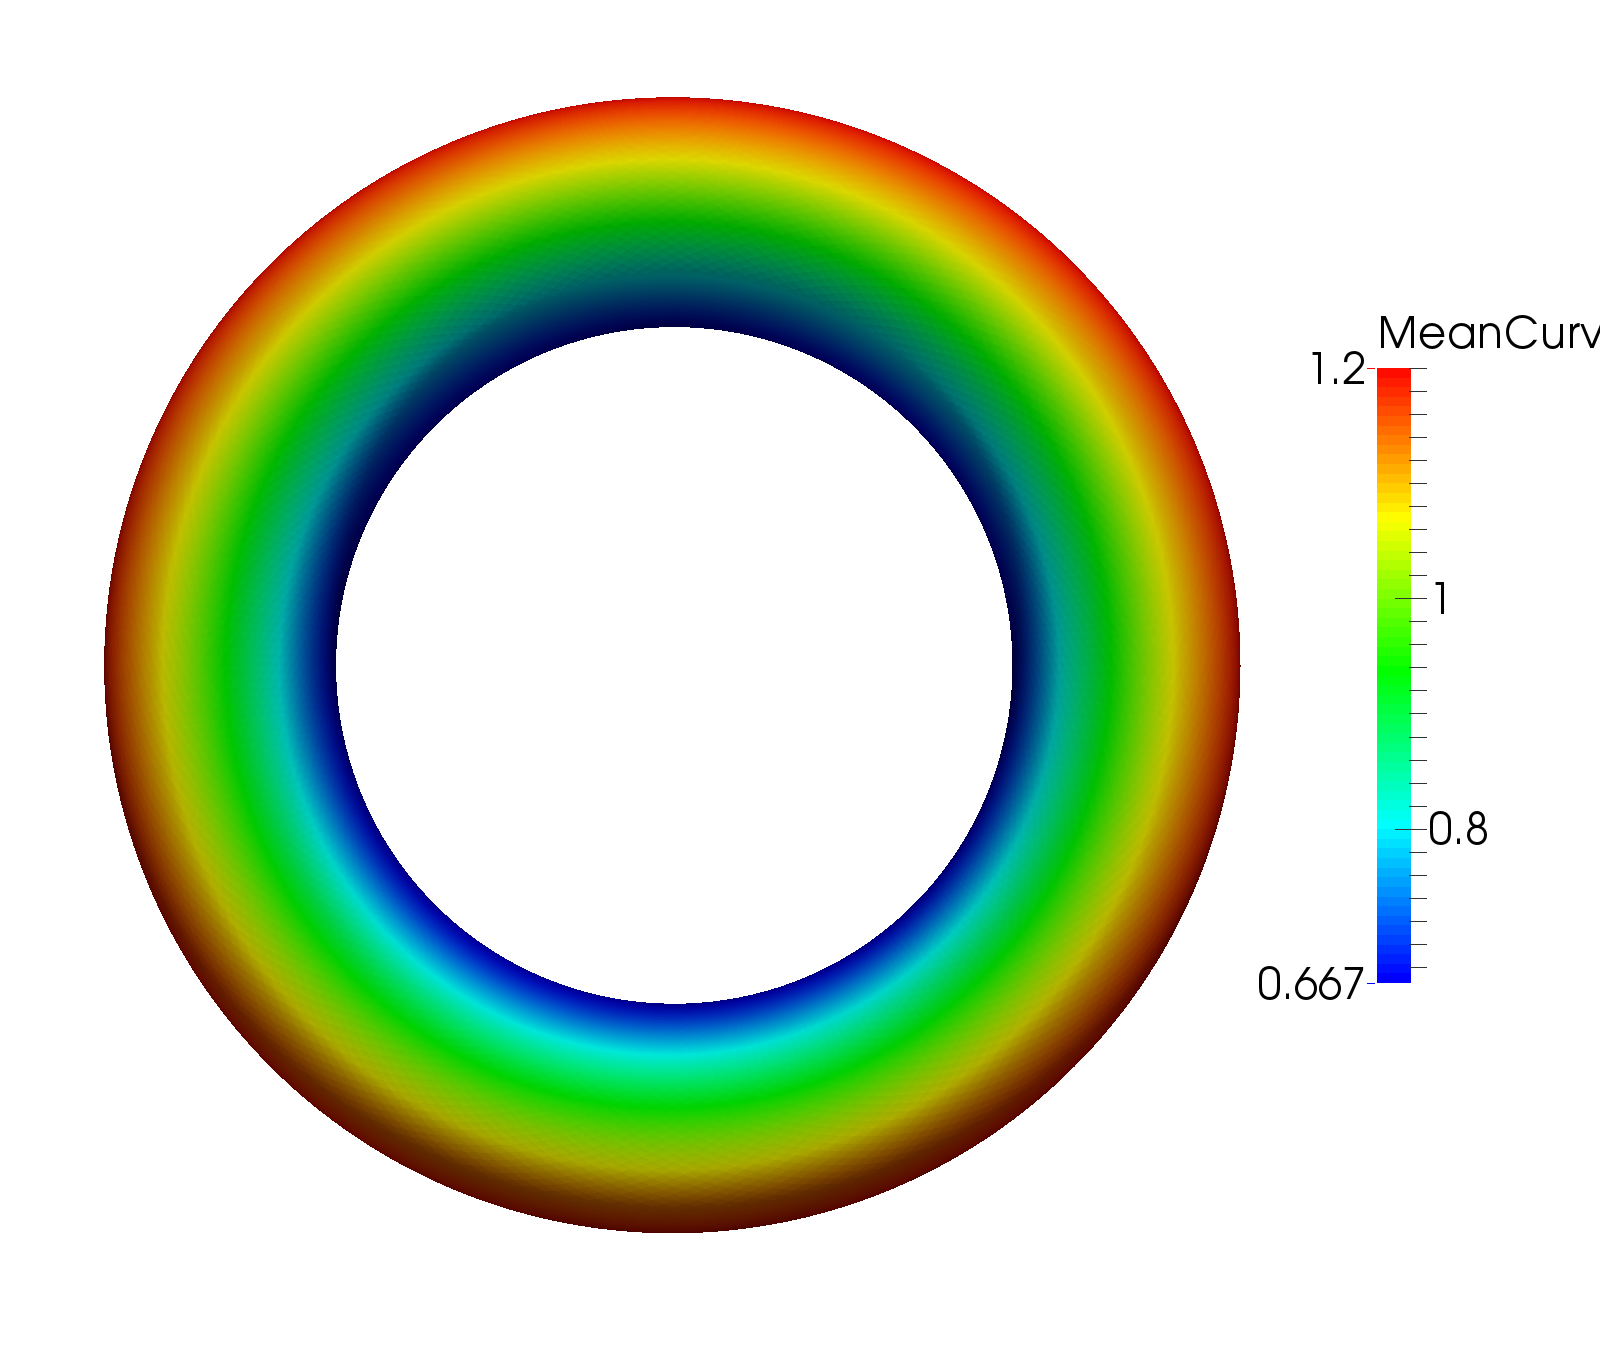
\includegraphics[width=\textwidth]{bilder/Curvature/WeinMeanTorus_25k.png}
        \end{minipage} \hfill
        \begin{minipage}[t]{0.49\textwidth}
          \centering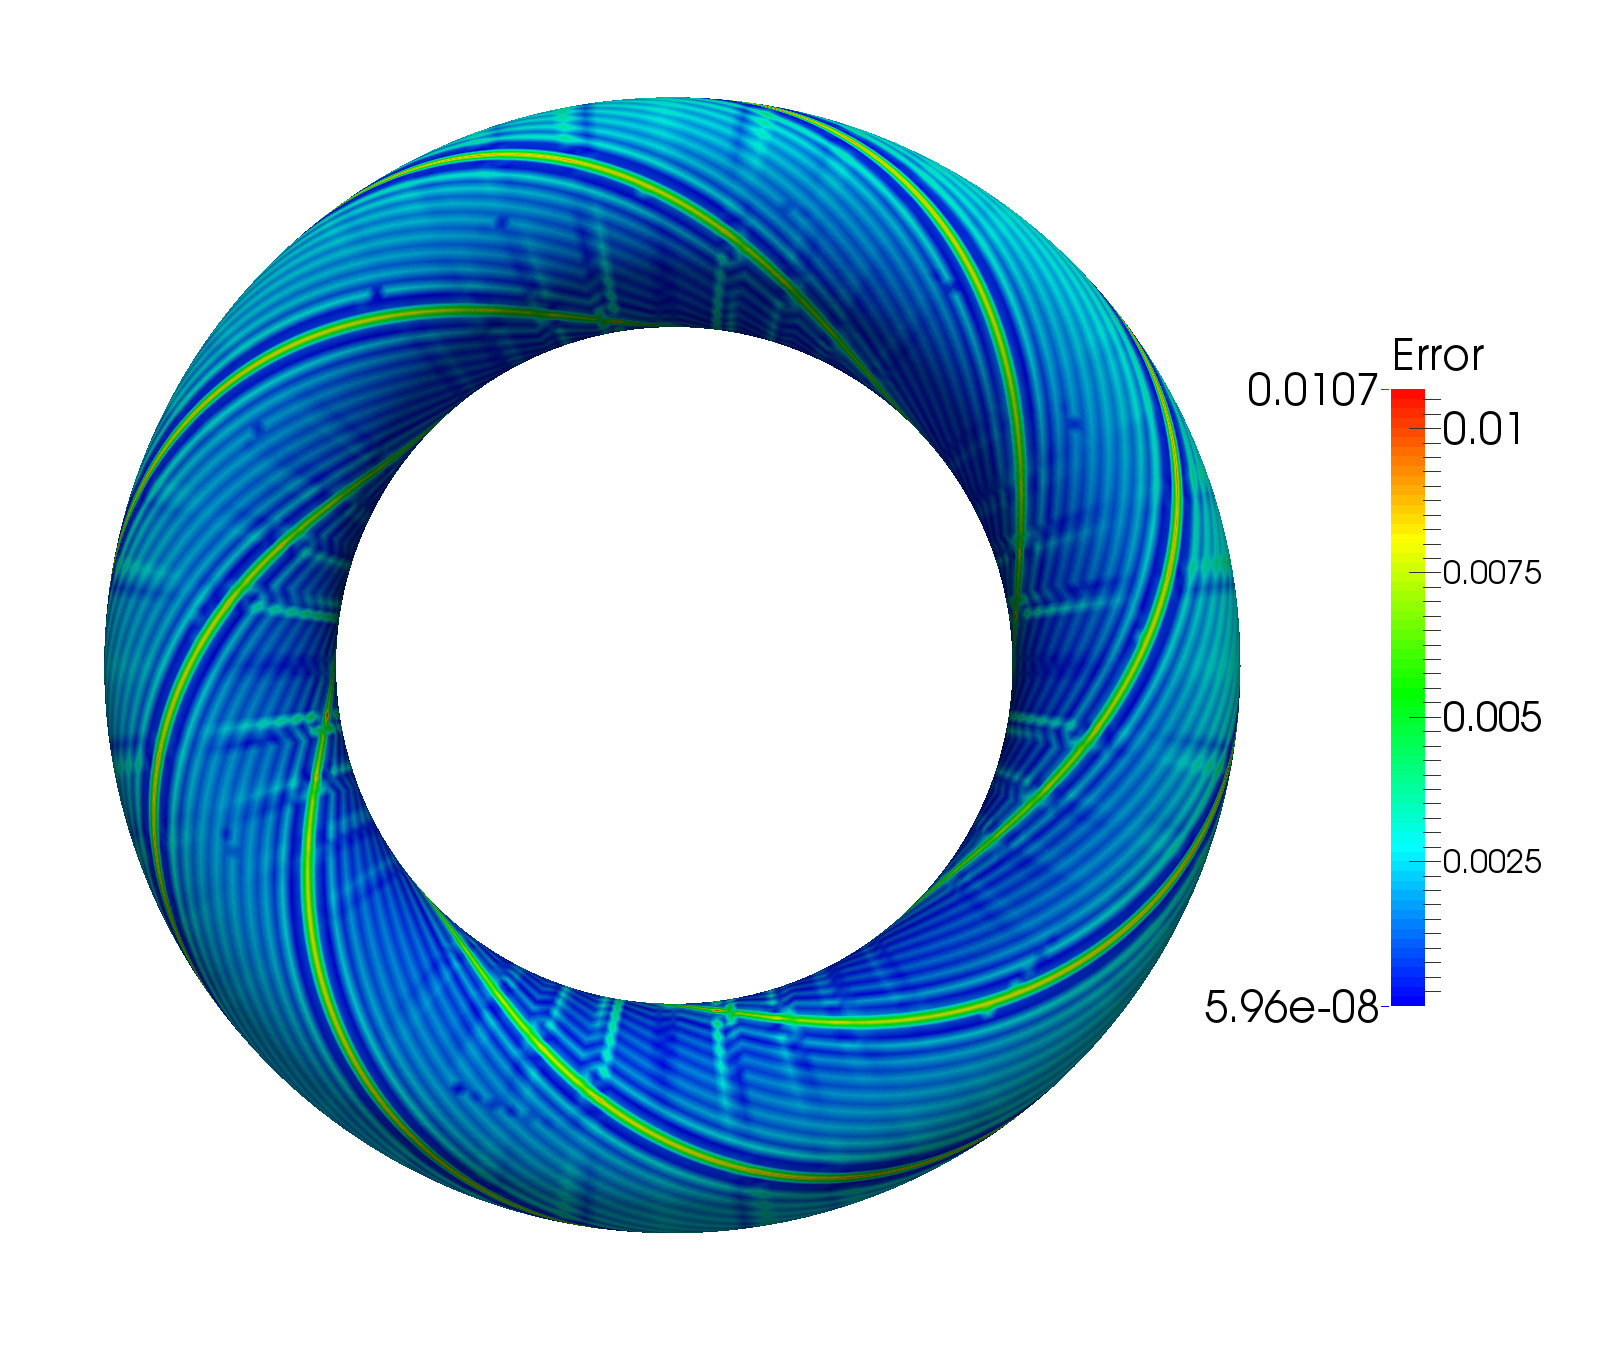
\includegraphics[width=\textwidth]{bilder/Curvature/WeinMeanTorusError_25k.png}
        \end{minipage}
        \caption[Mittlere Krümmung aus Weingartenabb. auf Torus]
                {Links: Mittlere Krümmung \( H \).
                 Rechts: Lokaler absoluter Fehler für die Bestimmung von \( H \) über die Weingartenabbildung mit gemittelten Normalen
                 \eqref{eqNormalMittel}. Das Gitter hat 24640 DOFs (\( h\approx 0.06 \)). 
                 Ab dieser Gitterauflösung fängt die Konvergenzrate an stark zu stagnieren.
                 Deutlich sind wieder die Verdrillungsstrukturen des Torus zu sehen.}
       \label{figMeanTorus}
    \begin{minipage}[t]{0.49\textwidth}
       \centering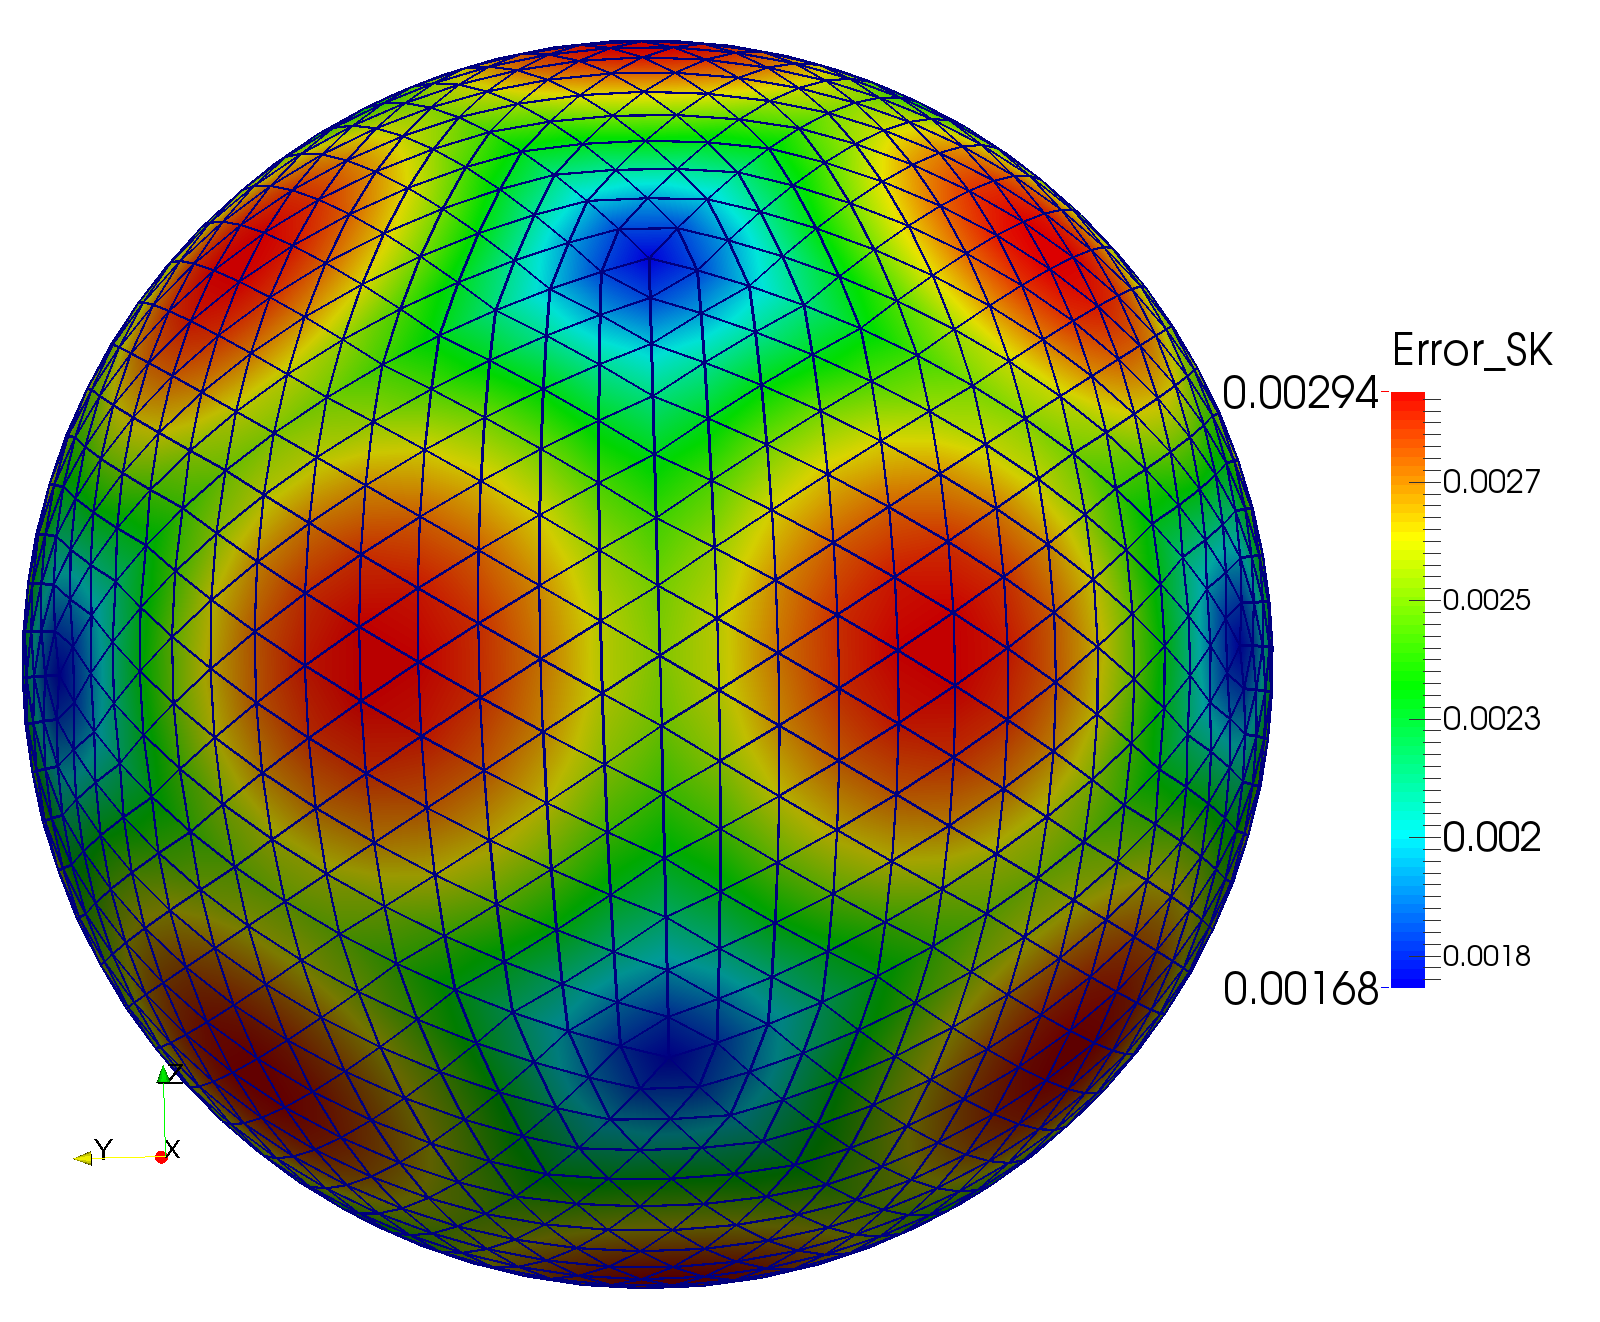
\includegraphics[width=\textwidth]{bilder/Curvature/sphere/ErrSK2k.png}
    \end{minipage}\hfill
    \begin{minipage}[t]{0.49\textwidth}
       \centering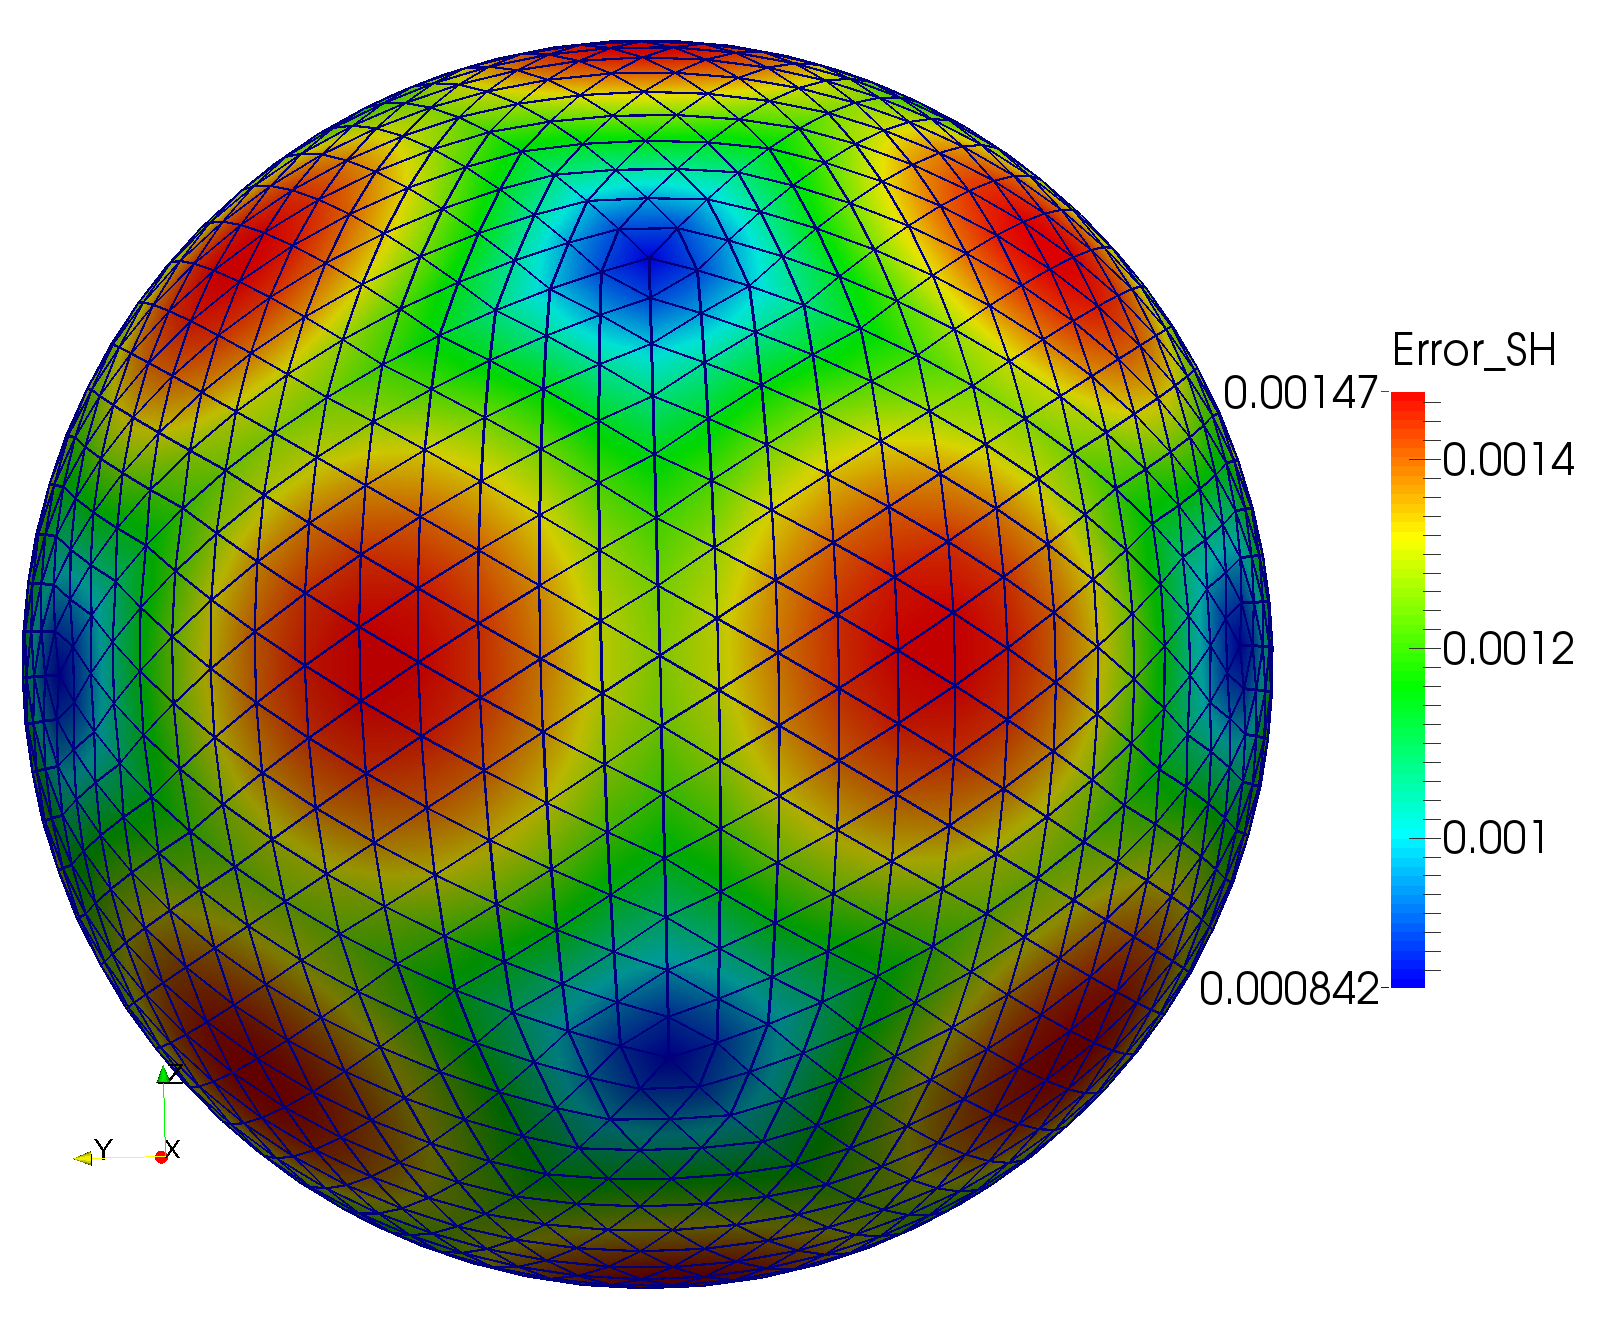
\includegraphics[width=\textwidth]{bilder/Curvature/sphere/ErrSH2k.png}
    \end{minipage}\\
    \begin{minipage}[t]{0.49\textwidth}
       \centering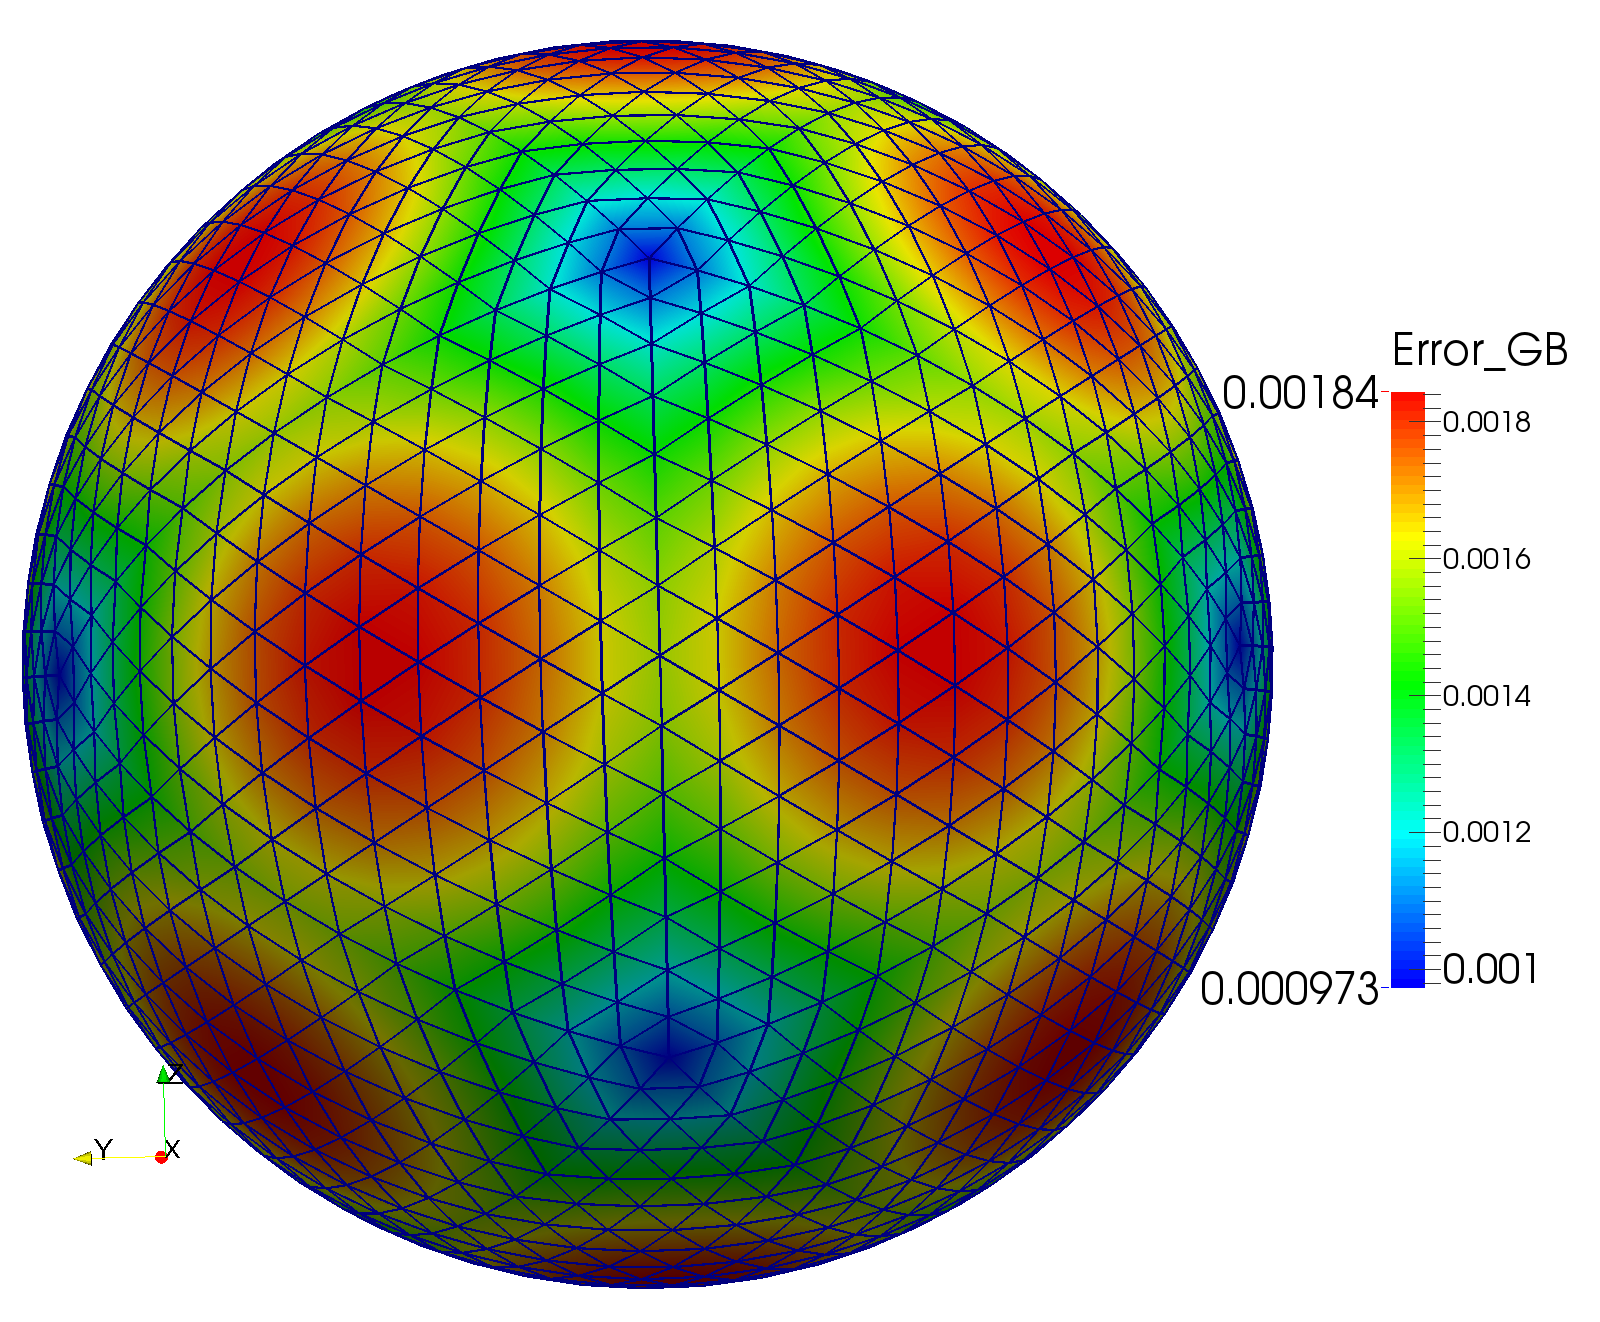
\includegraphics[width=\textwidth]{bilder/Curvature/sphere/ErrGB2k.png}
    \end{minipage}\hfill
    \begin{minipage}[t]{0.49\textwidth}
       \centering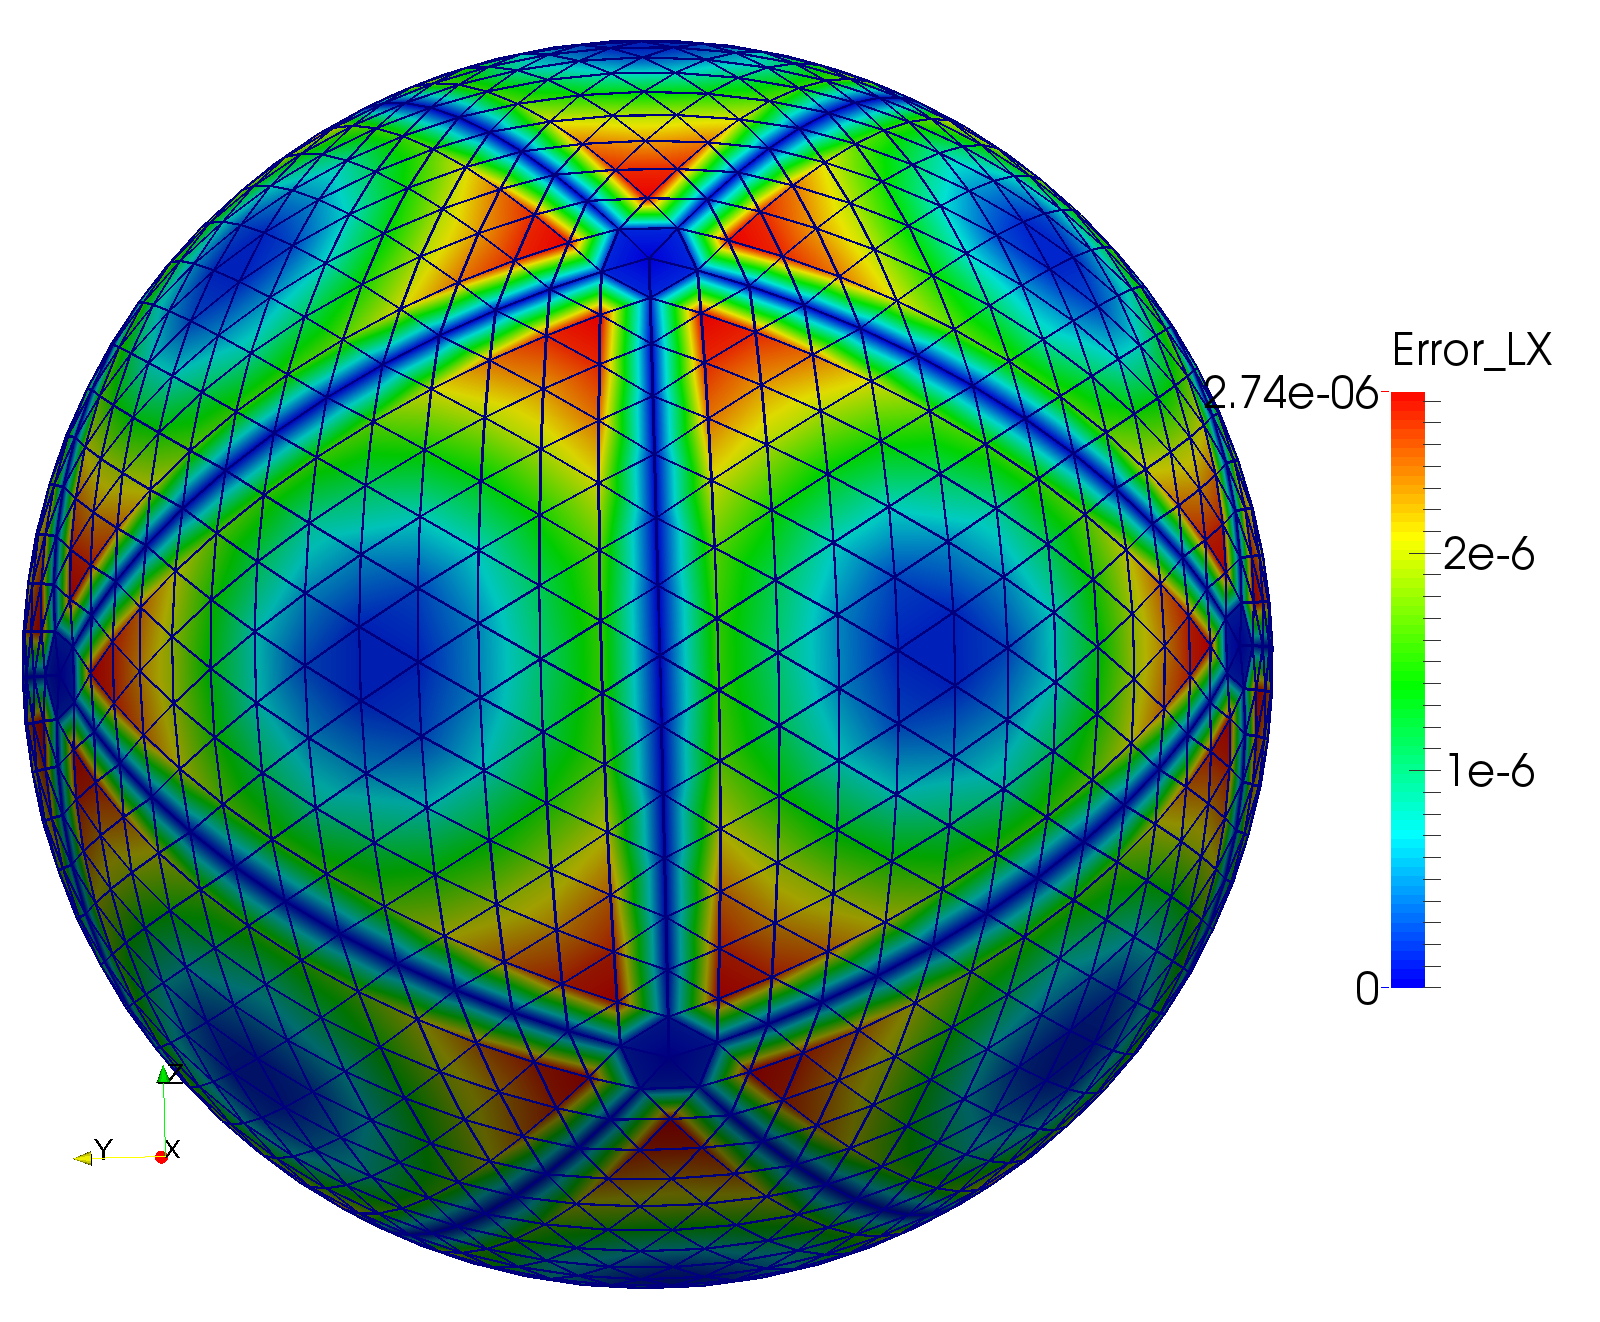
\includegraphics[width=\textwidth]{bilder/Curvature/sphere/ErrLX2k.png}
    \end{minipage}
    \caption[Fehler (Krümmungen auf Sphäre)]
            {Absolute lokale Fehler für die Gaußsche Krümmung (links) und mittlere Krümmung (rechts) auf der Sphäre
             ermittelt aus den Eigenwerten der diskreten Weingartenabbildung (oben), dem
             Gauß-Bonnet-Operator (unten links) bzw. dem Krümmungsvektor (unten rechts).
             (1962 DOFs, \( h\approx0.11 \))}
    \label{figErrCurvSphere}
  \end{figure}

  \begin{figure}
    \begin{minipage}[t]{0.49\textwidth}
       \centering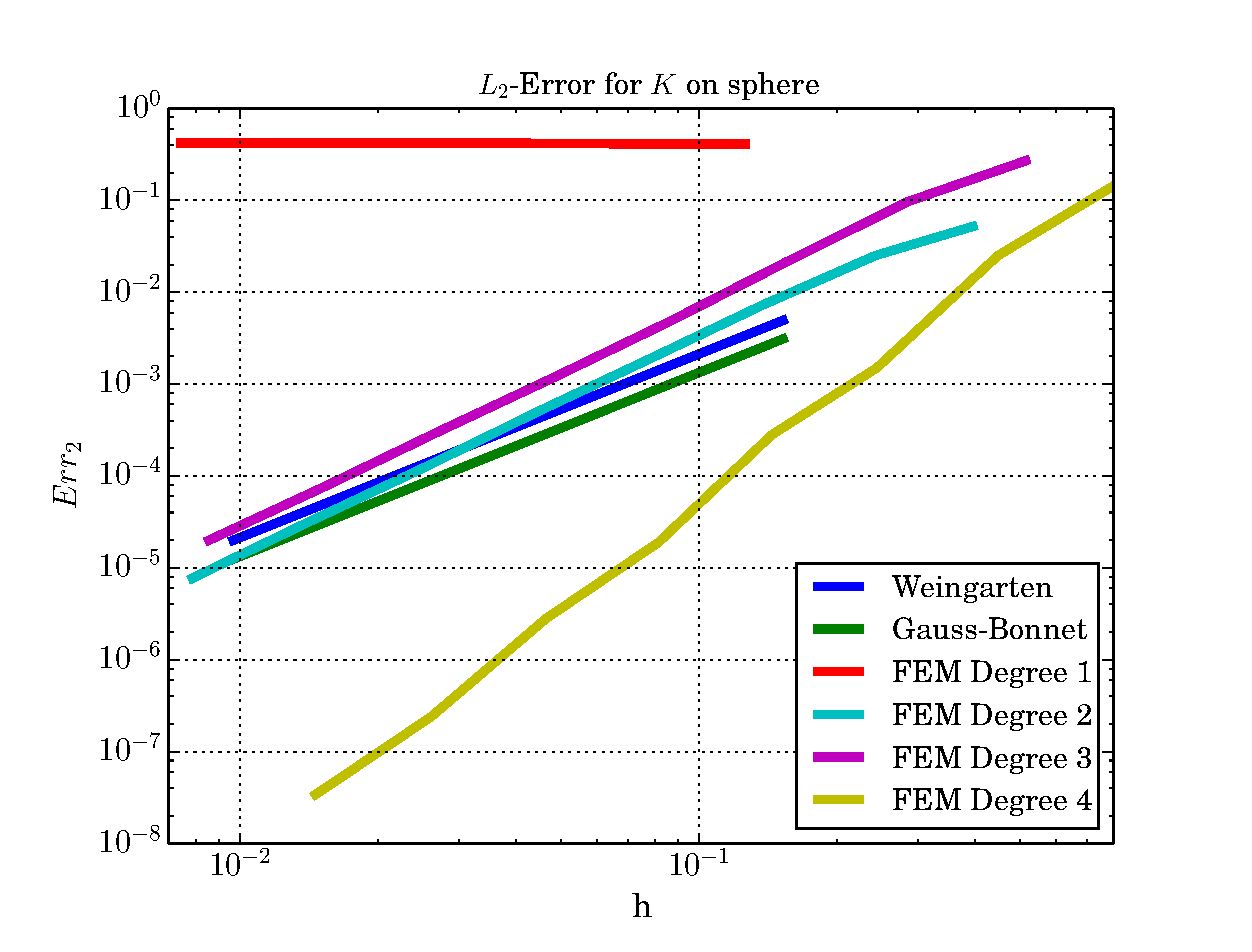
\includegraphics[width=\textwidth]{bilder/Curvature/sphere/ErrKL2.eps}
    \end{minipage}\hfill
    \begin{minipage}[t]{0.49\textwidth}
       \centering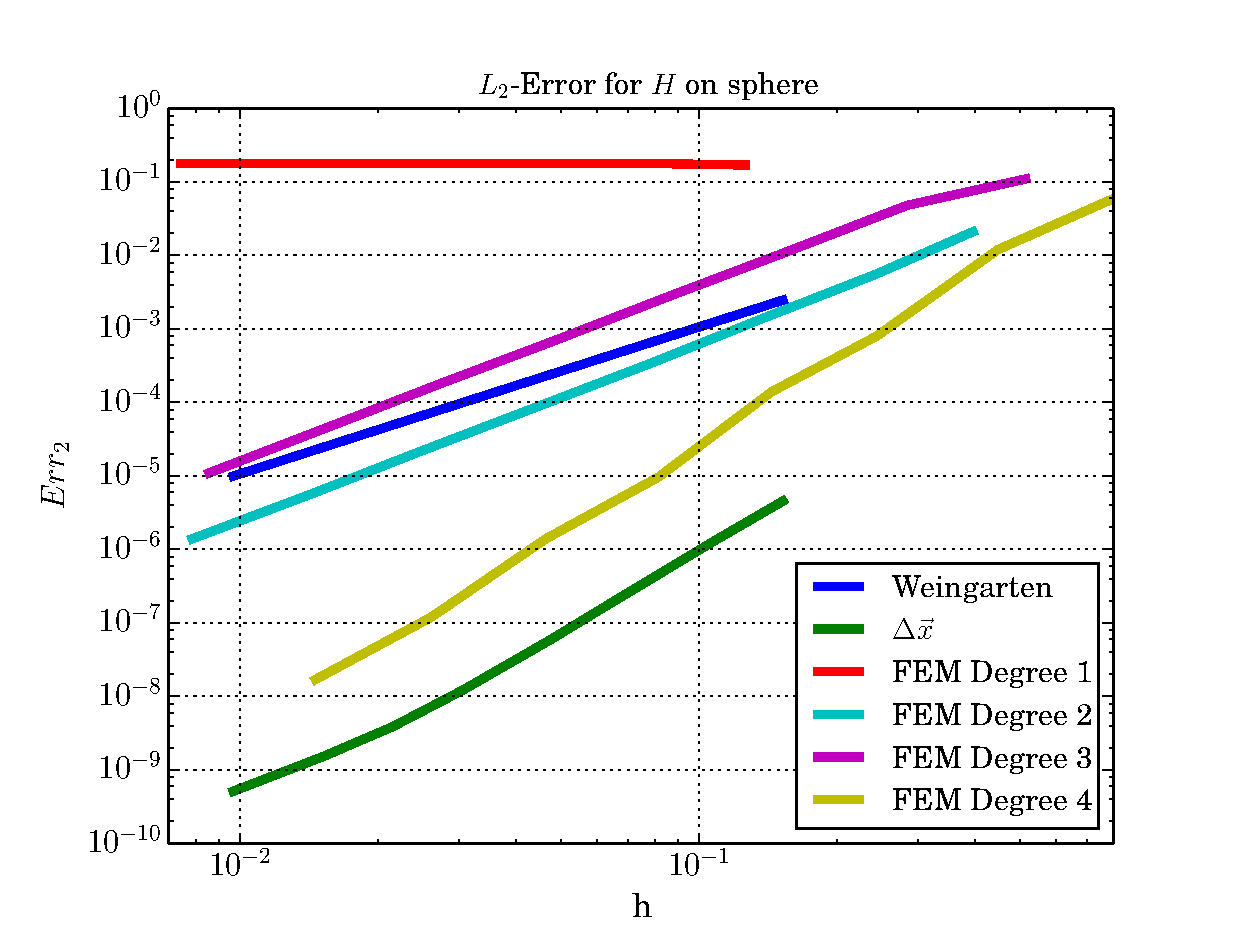
\includegraphics[width=\textwidth]{bilder/Curvature/sphere/ErrHL2.eps}
    \end{minipage}\\
    \begin{minipage}[t]{0.49\textwidth}
       \centering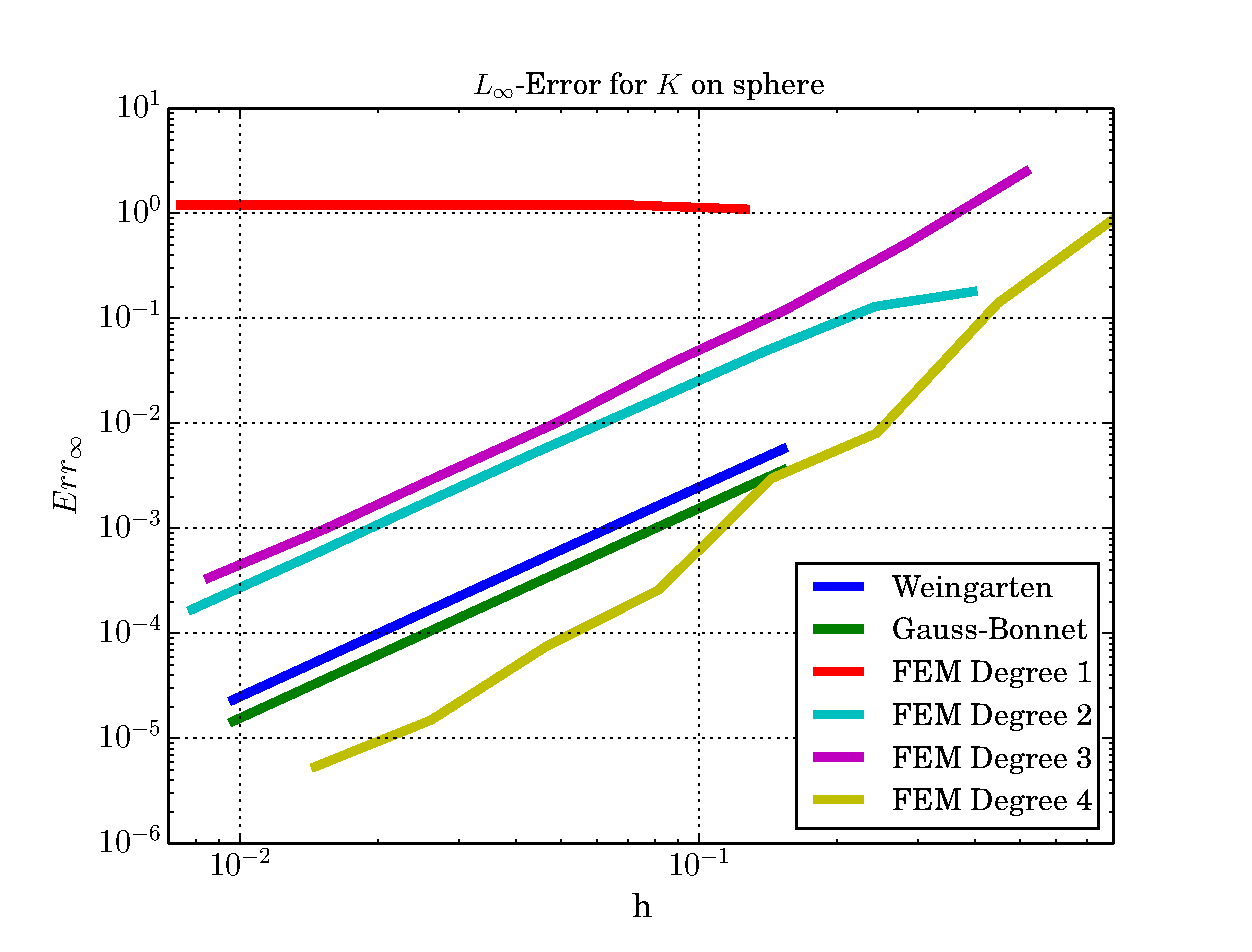
\includegraphics[width=\textwidth]{bilder/Curvature/sphere/ErrKLMax.eps}
    \end{minipage}\hfill
    \begin{minipage}[t]{0.49\textwidth}
       \centering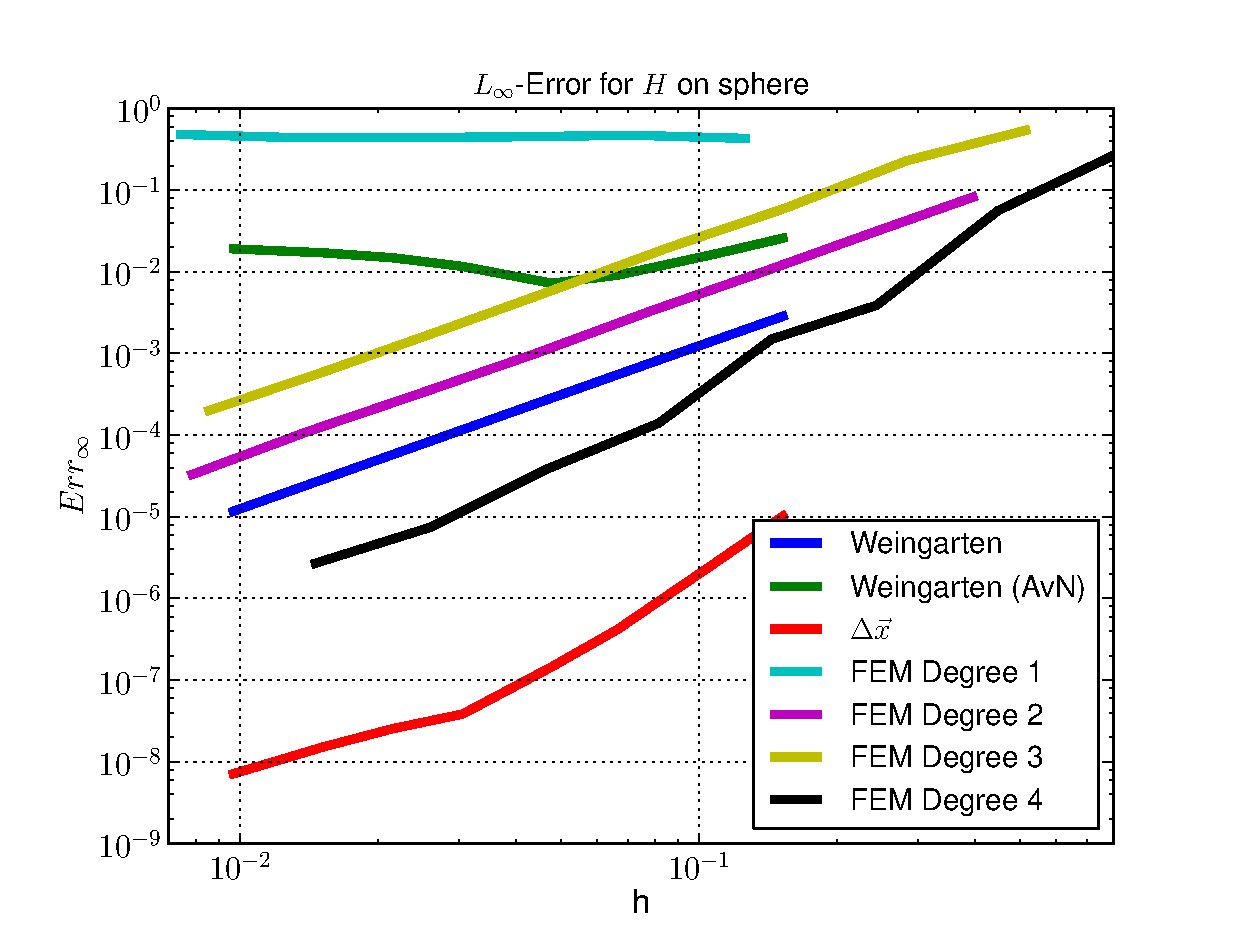
\includegraphics[width=\textwidth]{bilder/Curvature/sphere/ErrHLMax.eps}
    \end{minipage}
    \caption[Fehlerplot (Krümmungen auf Sphäre)]
            {Log-Log-Plot der relativen diskreten \( L_{2} \)-Fehler (oben) und Maximumsfehler (unten) 
             für die Gaußsche Krümmung (links) und mittlere Krümmung (rechts) auf der Sphäre.}
    \label{figErrCompSphere}
    \centering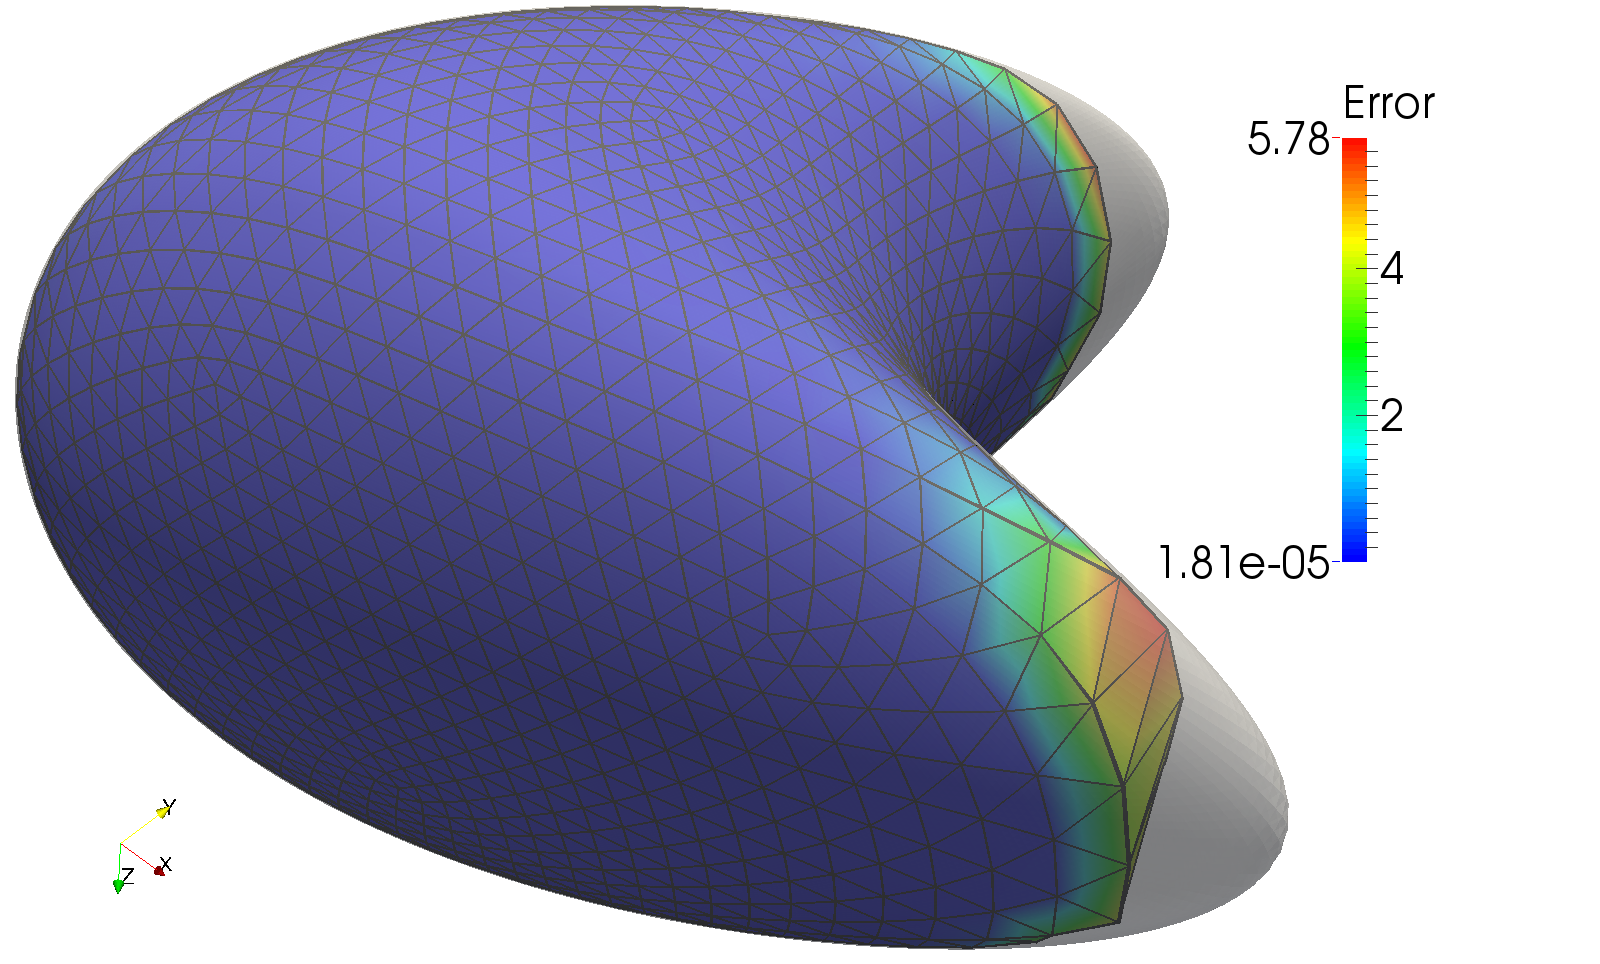
\includegraphics[width=\textwidth]{bilder/Curvature/HeineB2k250kMeshGaussError.png}
    \caption[Gitterauflösung (quatrische Oberfläche)]
            {Das Gitter mit 1962 DOFs (\( h\approx0.34 \)) löst die beiden Wölbungen mit starker Krümmung
            nicht auf. Der Fehler (hier für \( K \) (Weingarten)) ist dort am größten. 
            Zum Vergleich ist ein Gitter mit 249642 DOFs (\( h\approx0.04 \)) halbtransparent
            dargestellt.}
    \label{figHeineBResolution}
  \end{figure}

  \begin{figure}
    \begin{minipage}[t]{0.49\textwidth}
       \centering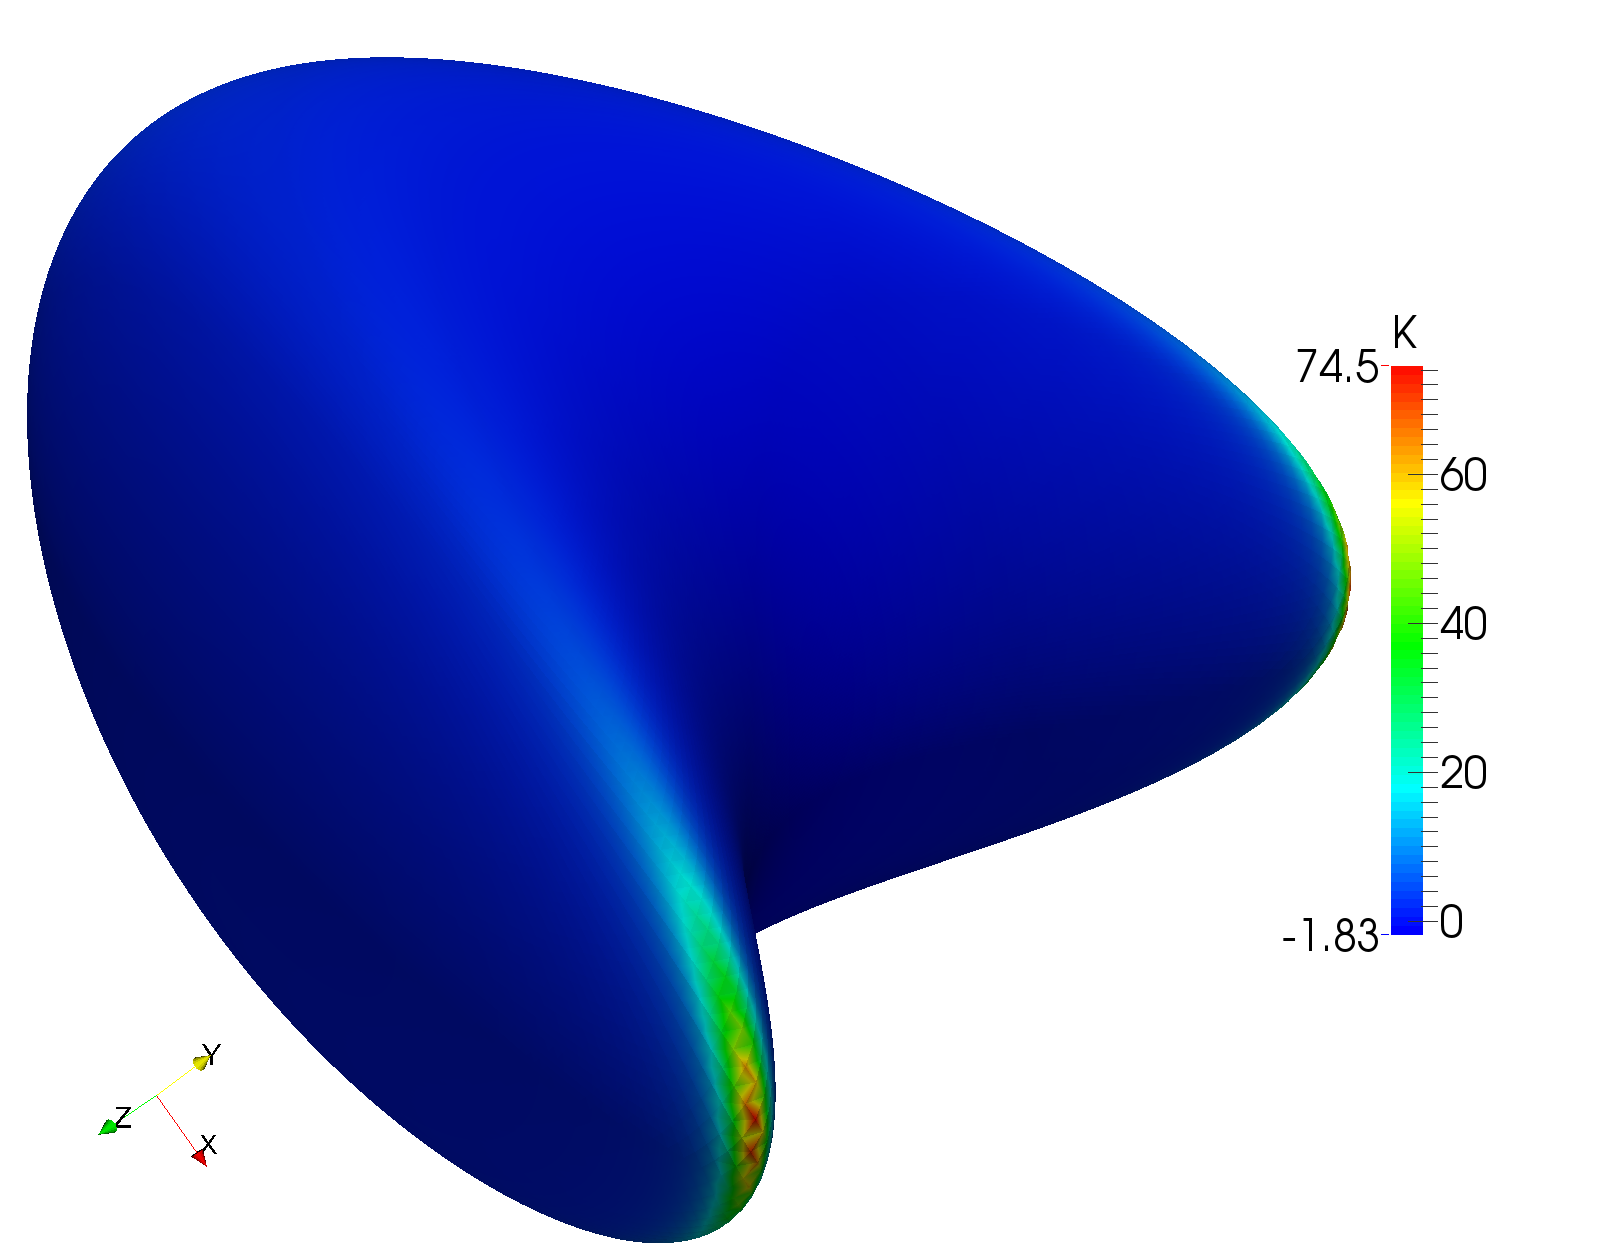
\includegraphics[width=\textwidth]{bilder/Curvature/heineB/K250k.png}
    \end{minipage}\hfill
    \begin{minipage}[t]{0.49\textwidth}
       \centering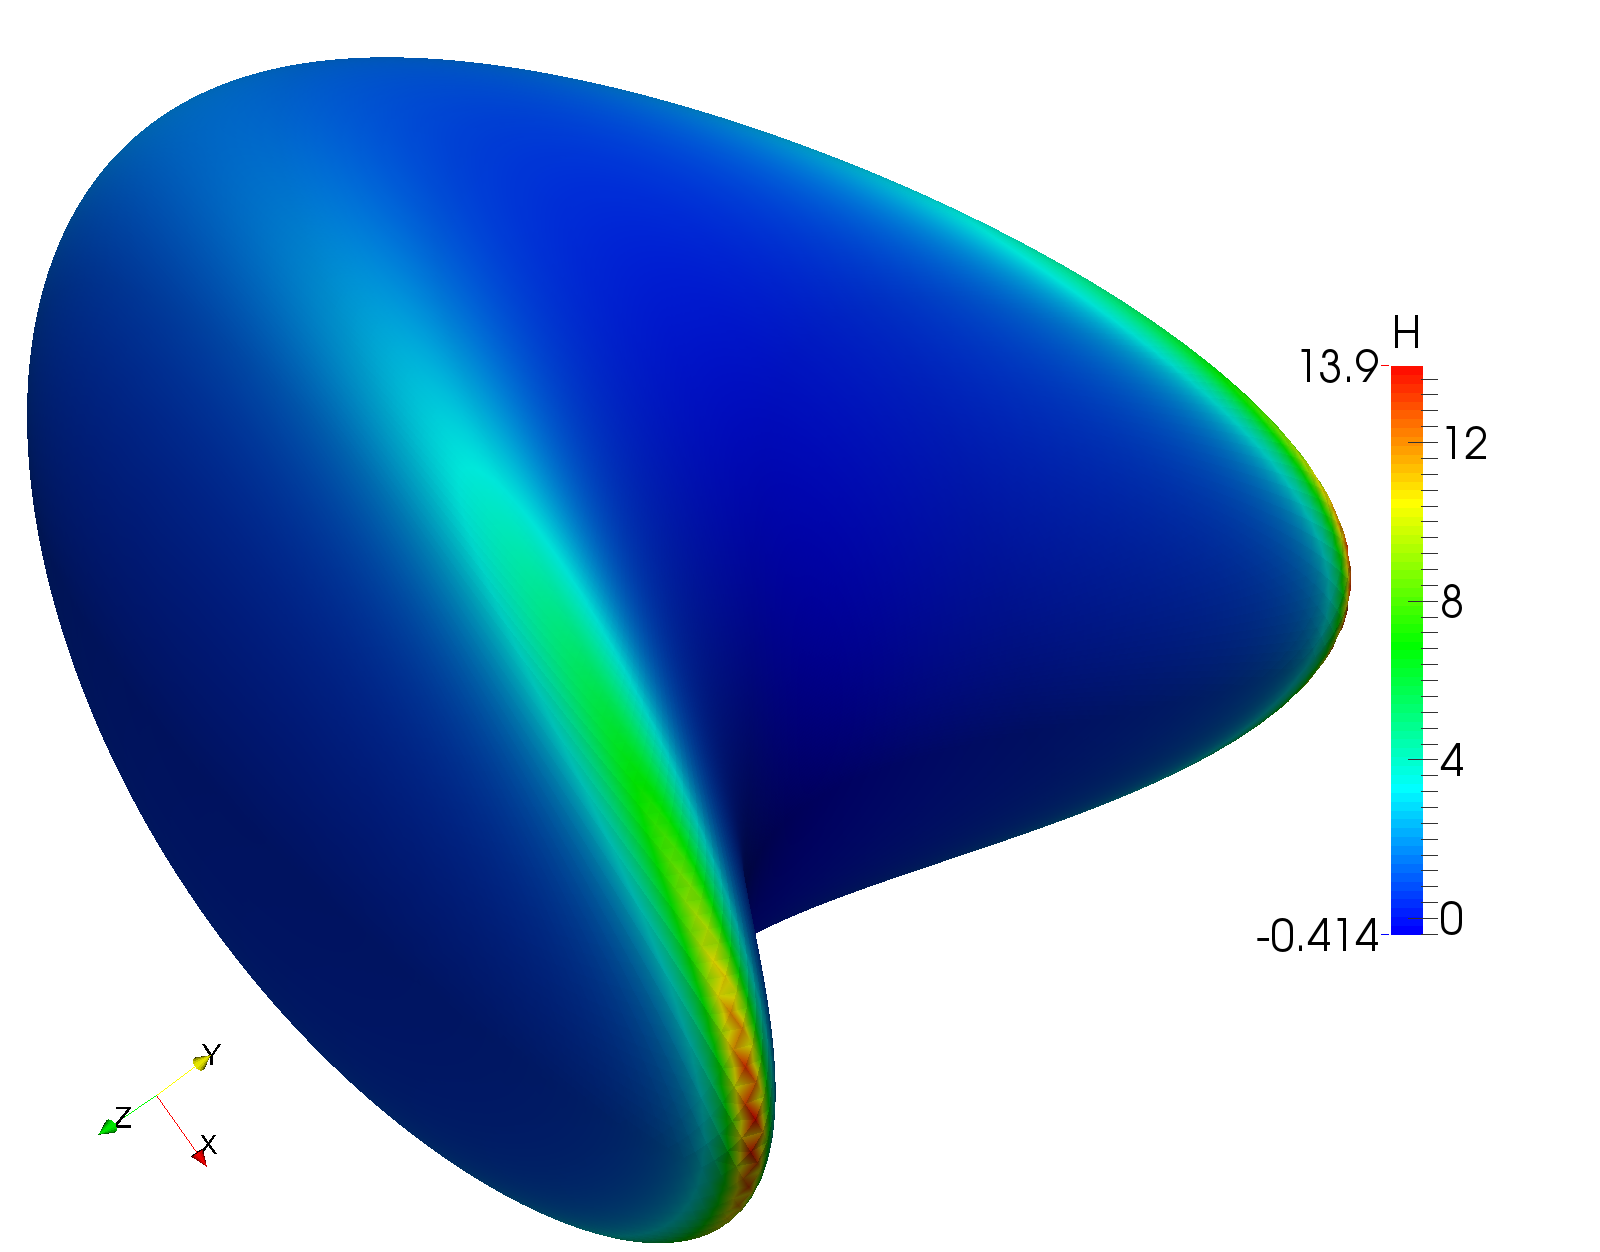
\includegraphics[width=\textwidth]{bilder/Curvature/heineB/H250k.png}
    \end{minipage}\\
    \begin{minipage}[t]{0.49\textwidth}
       \centering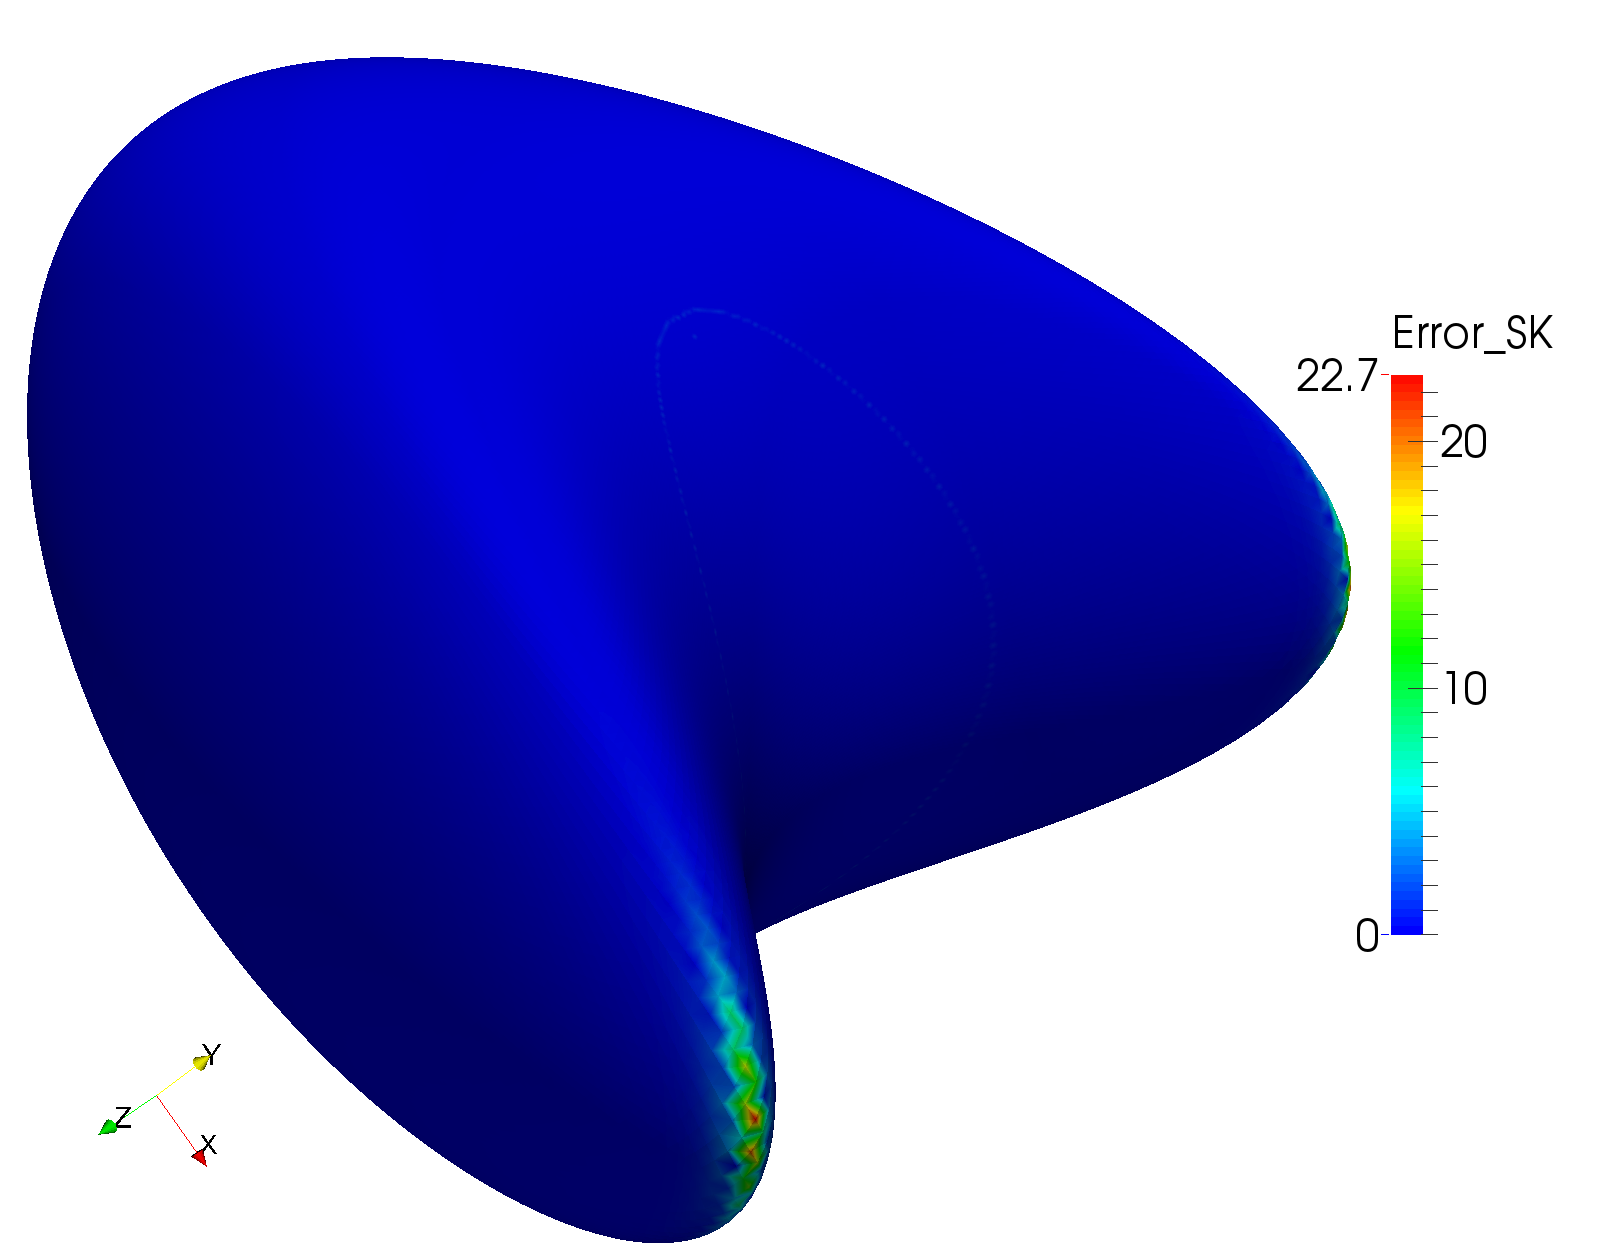
\includegraphics[width=\textwidth]{bilder/Curvature/heineB/SK250k.png}
    \end{minipage}\hfill
    \begin{minipage}[t]{0.49\textwidth}
       \centering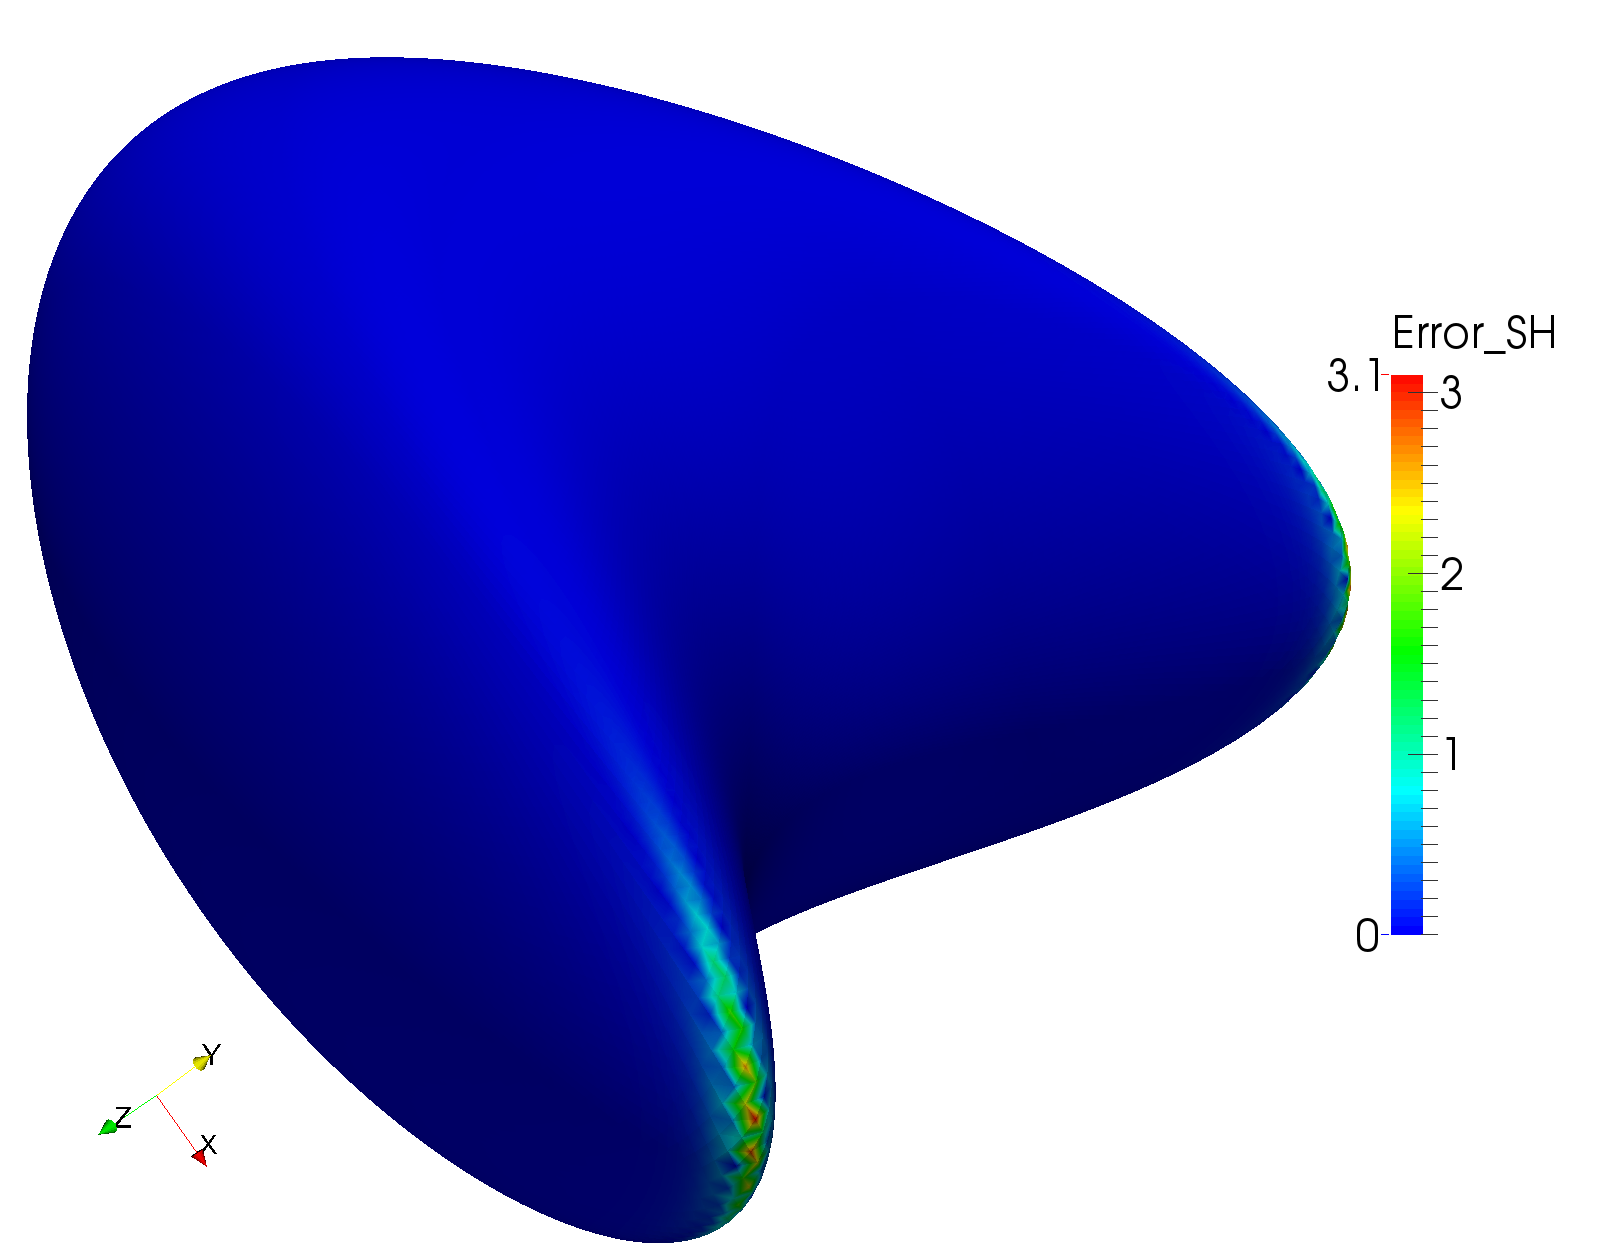
\includegraphics[width=\textwidth]{bilder/Curvature/heineB/SH250k.png}
    \end{minipage}\\
    \begin{minipage}[t]{0.49\textwidth}
       \centering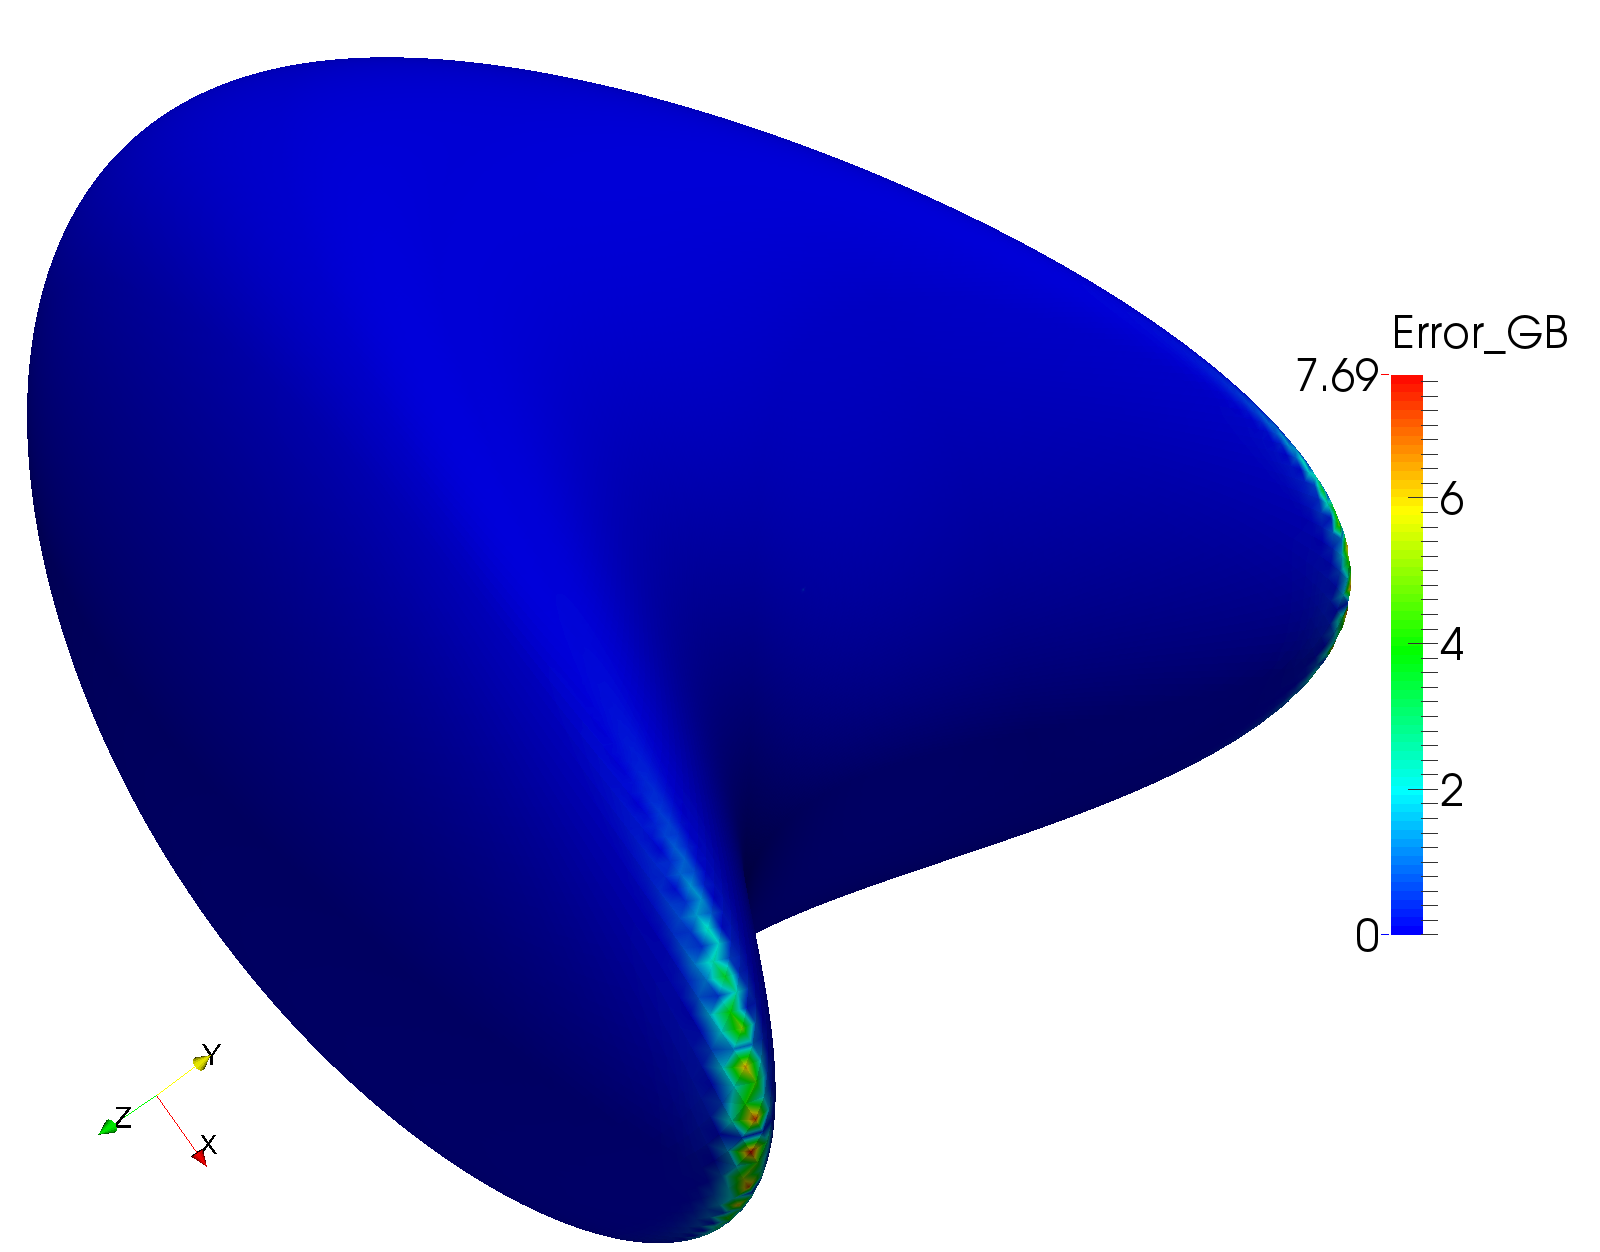
\includegraphics[width=\textwidth]{bilder/Curvature/heineB/GB250k.png}
    \end{minipage}\hfill
    \begin{minipage}[t]{0.49\textwidth}
       \centering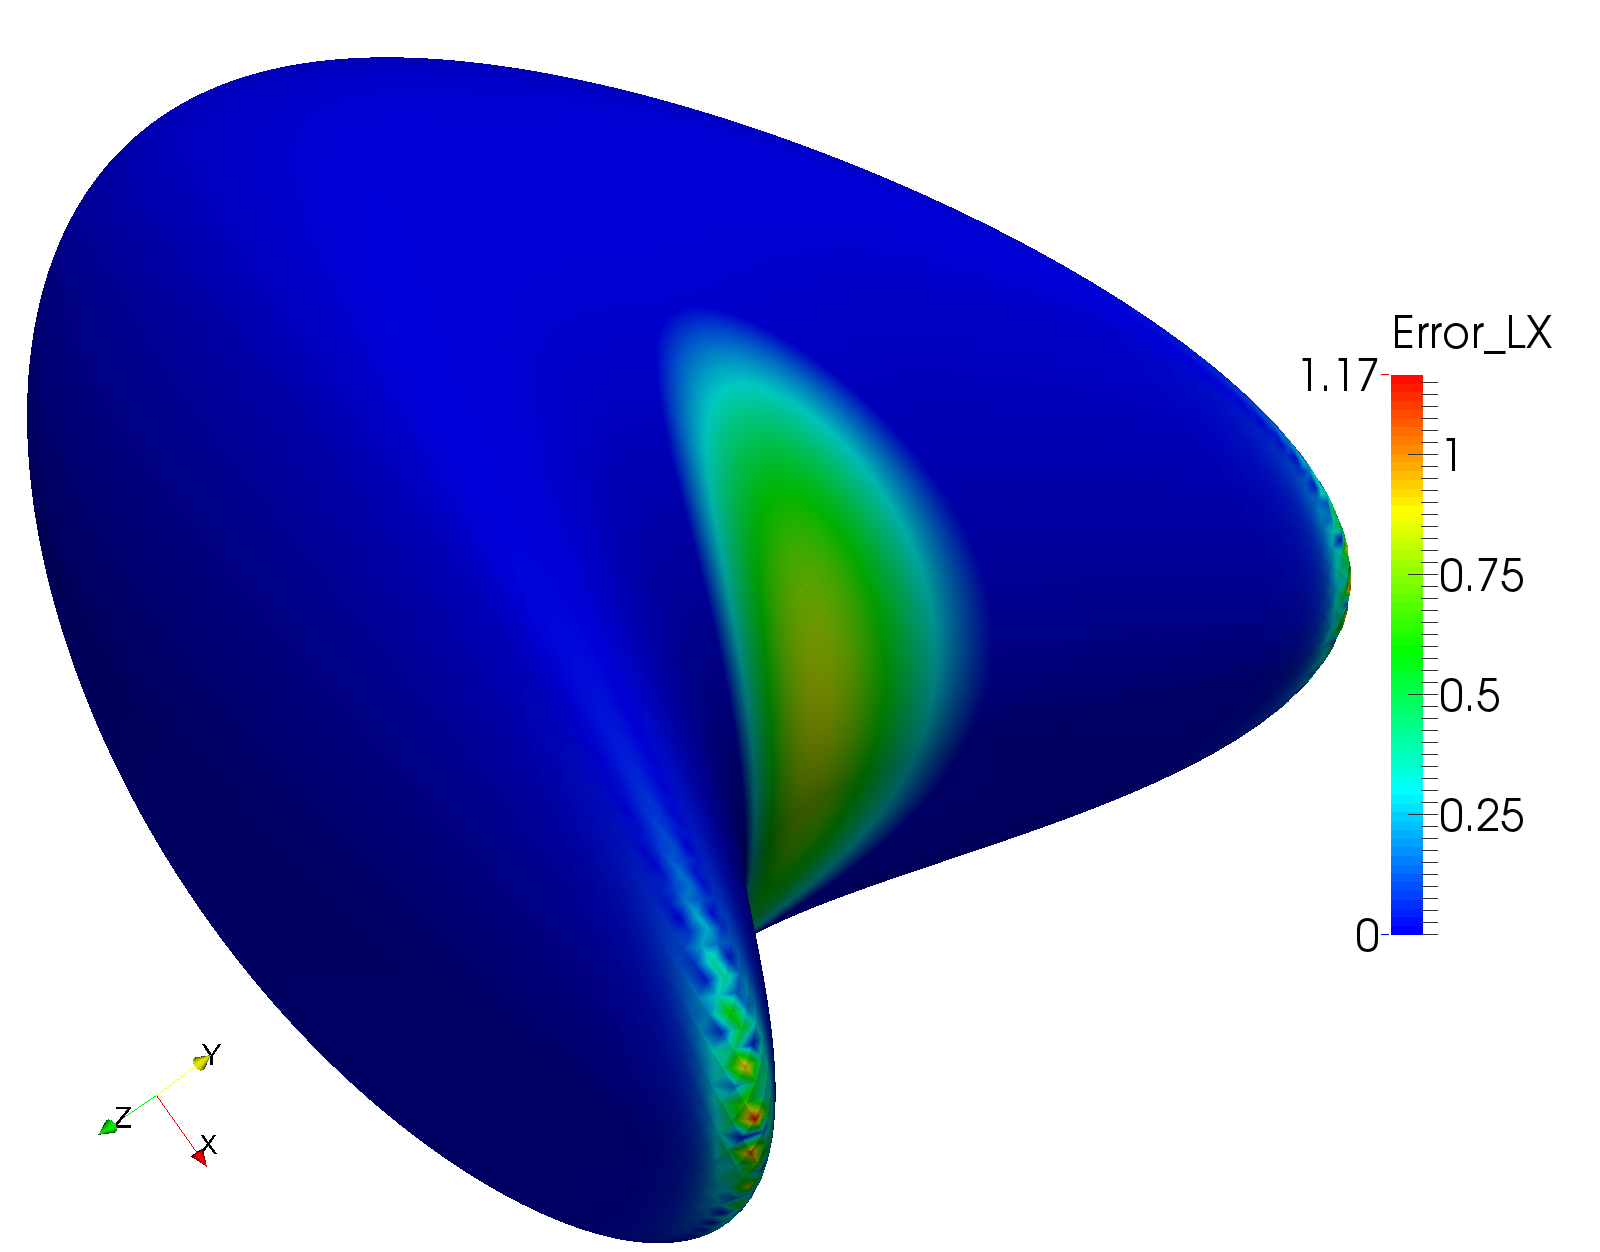
\includegraphics[width=\textwidth]{bilder/Curvature/heineB/LX250k.png}
    \end{minipage}
    \caption[Fehler (Krümmungen auf quatrischer Oberfläche)]
            {Absolute lokale Fehler für die Gaußsche Krümmung (links) und mittlere Krümmung (rechts) auf
            einer quatrischen Oberfläche
             ermittelt aus den Eigenwerten der diskreten Weingartenabbildung (Mitte), dem
             Gauß-Bonnet-Operator (unten links) bzw. dem Krümmungsvektor (unten rechts).
             (249642 DOFs, \( h\approx0.04 \))}
    \label{figErrCurvHeineB}
  \end{figure}

  \begin{figure}
    \begin{minipage}[t]{0.49\textwidth}
       \centering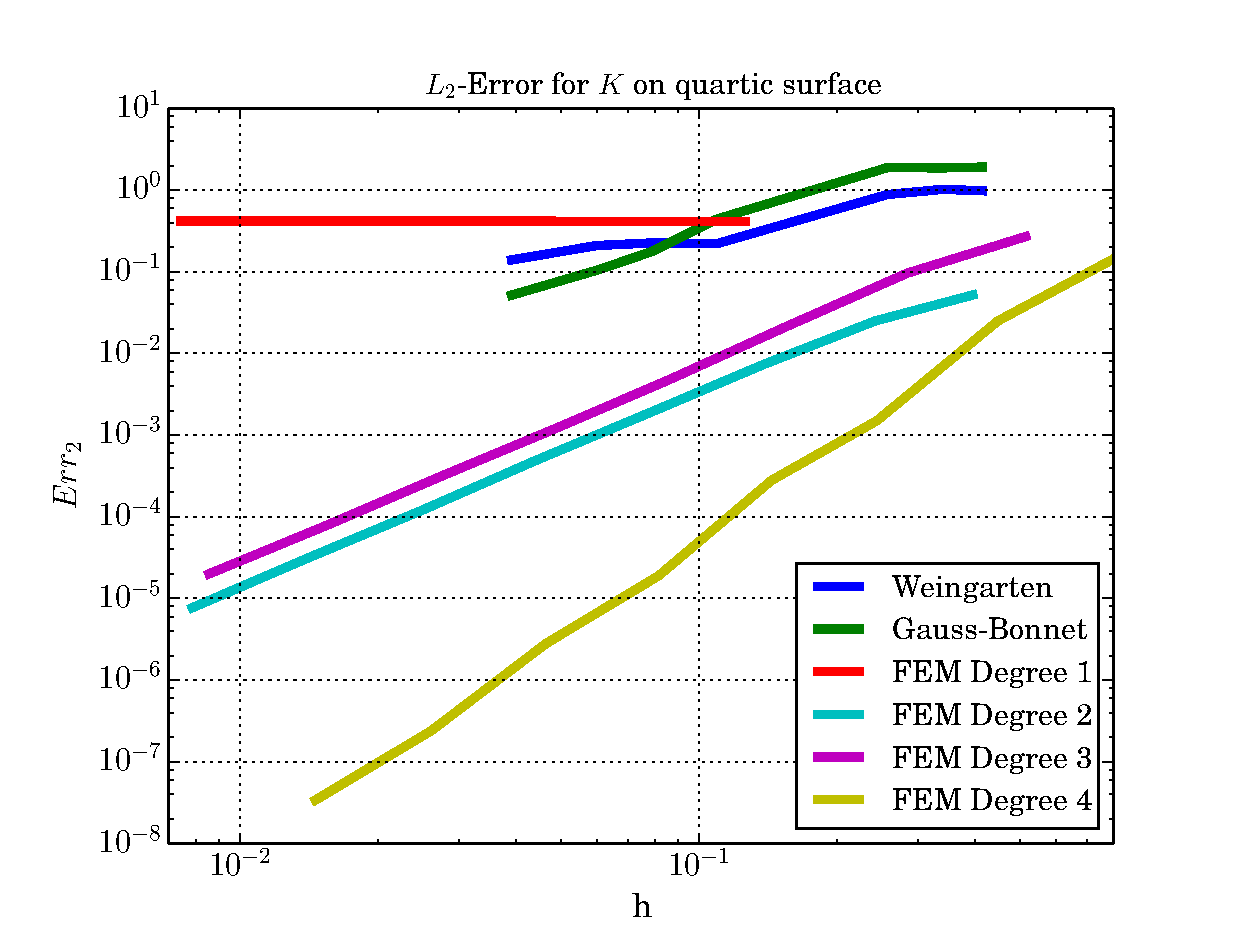
\includegraphics[width=\textwidth]{bilder/Curvature/heineB/ErrKL2.eps}
    \end{minipage}\hfill
    \begin{minipage}[t]{0.49\textwidth}
       \centering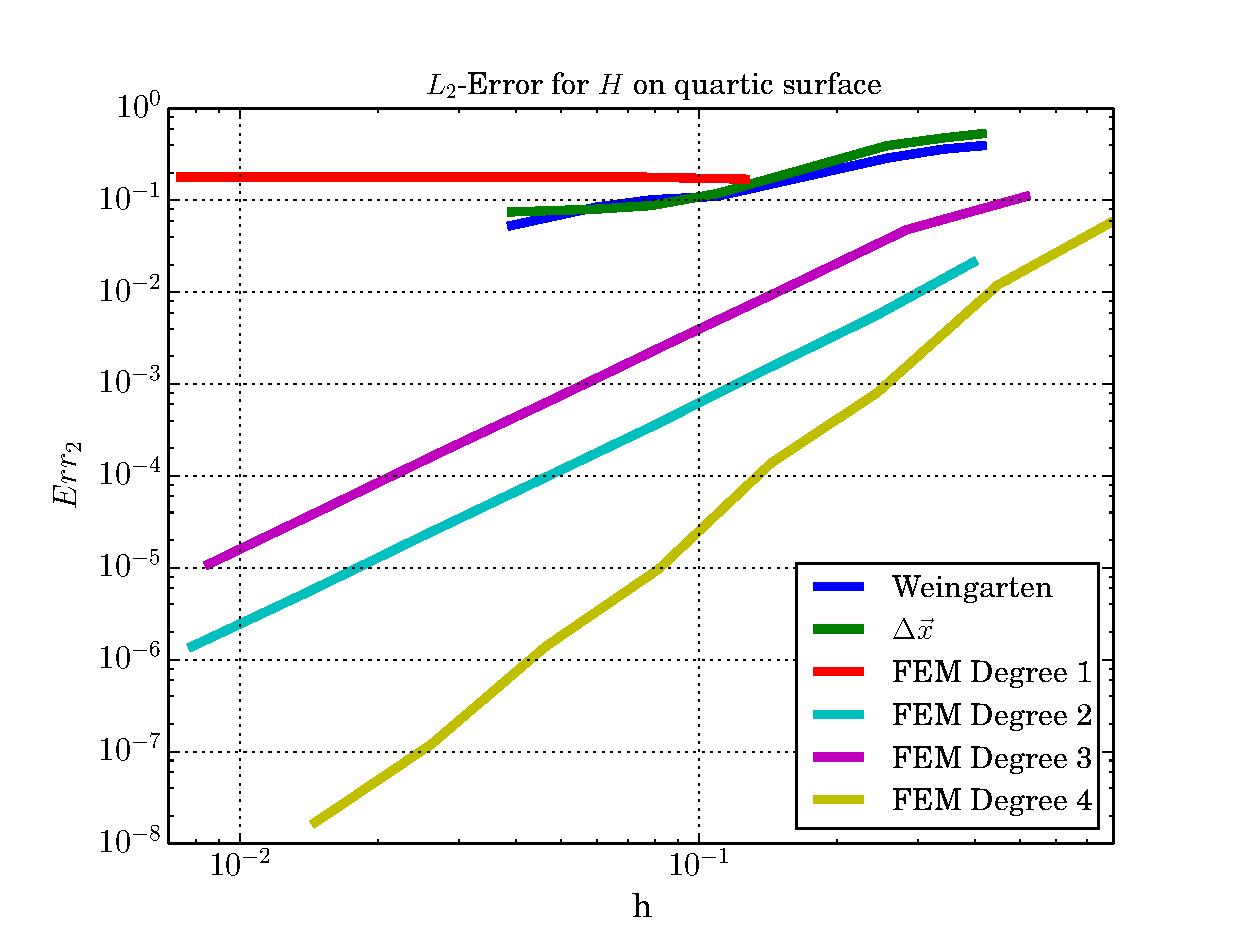
\includegraphics[width=\textwidth]{bilder/Curvature/heineB/ErrHL2.eps}
    \end{minipage}\\
    \begin{minipage}[t]{0.49\textwidth}
       \centering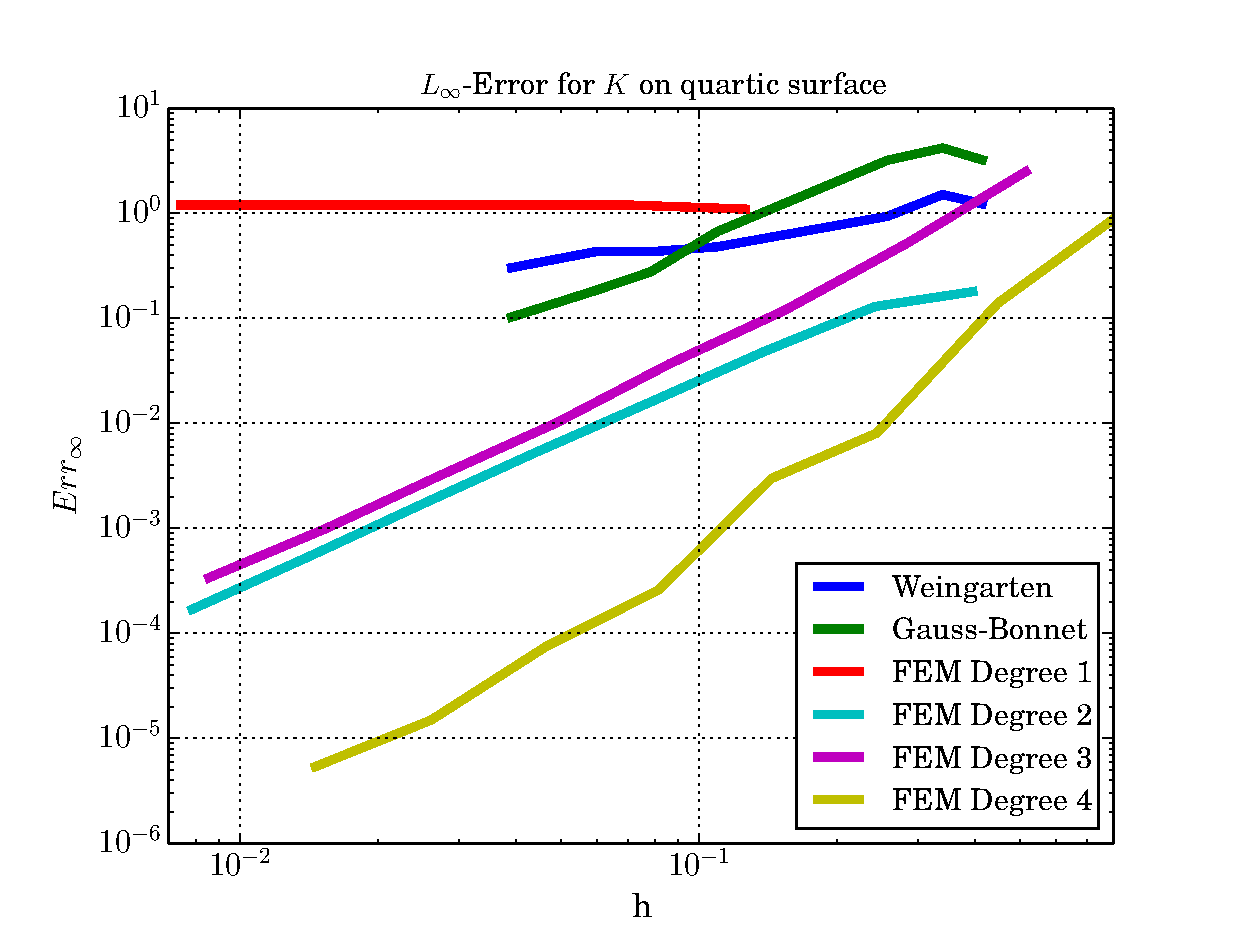
\includegraphics[width=\textwidth]{bilder/Curvature/heineB/ErrKMax.eps}
    \end{minipage}\hfill
    \begin{minipage}[t]{0.49\textwidth}
       \centering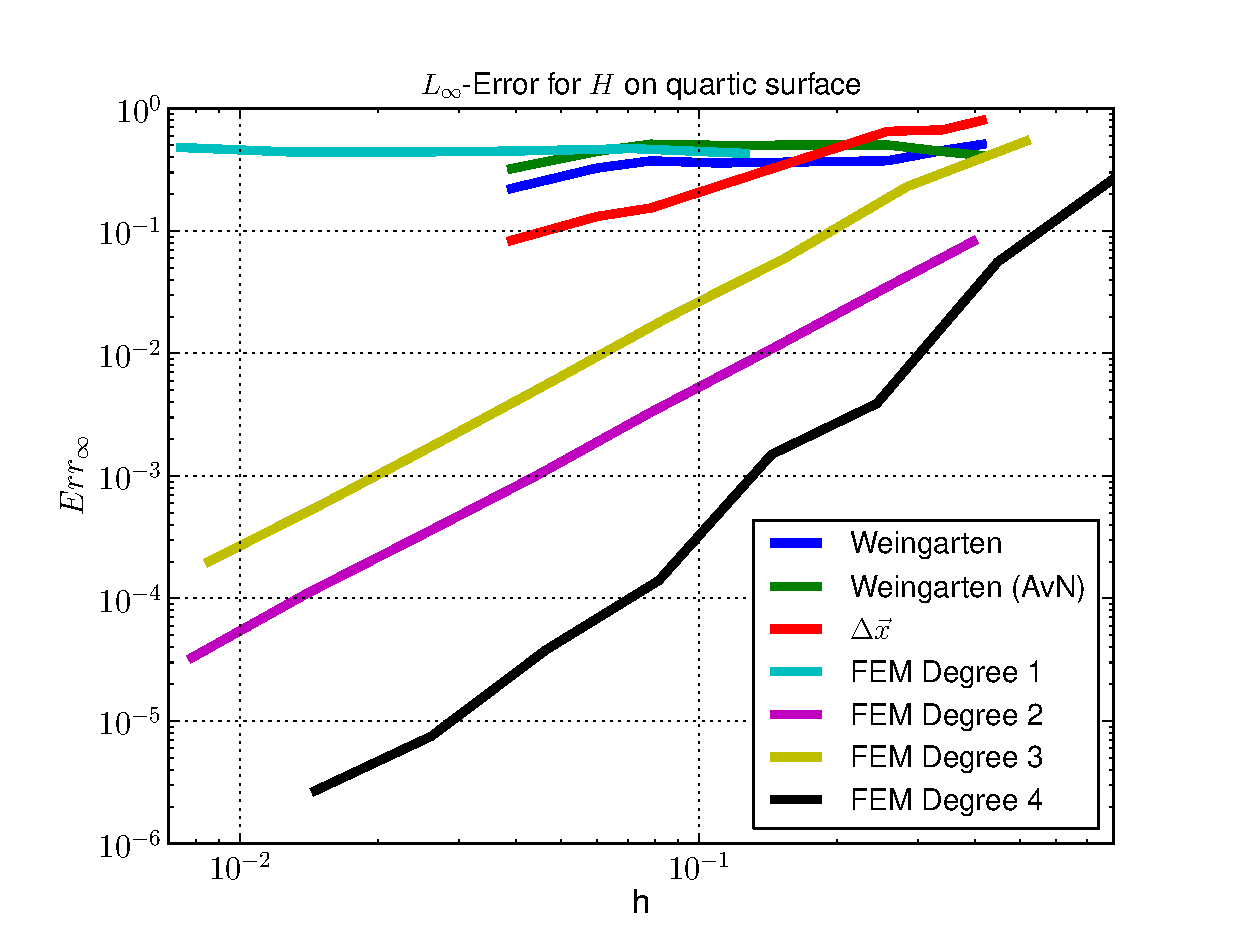
\includegraphics[width=\textwidth]{bilder/Curvature/heineB/ErrHMax.eps}
    \end{minipage}
    \caption[Fehlerplot (Krümmungen auf quatrischer Oberfläche)]
            {Log-Log-Plot der relativen diskreten \( L_{2} \)-Fehler (oben) und Maximumsfehler (unten) 
             für die Gaußsche Krümmung (links) und mittlere Krümmung (rechts) auf einer quatrischen
             Oberfläche.}
    \label{figErrCompHeineB}
    \centering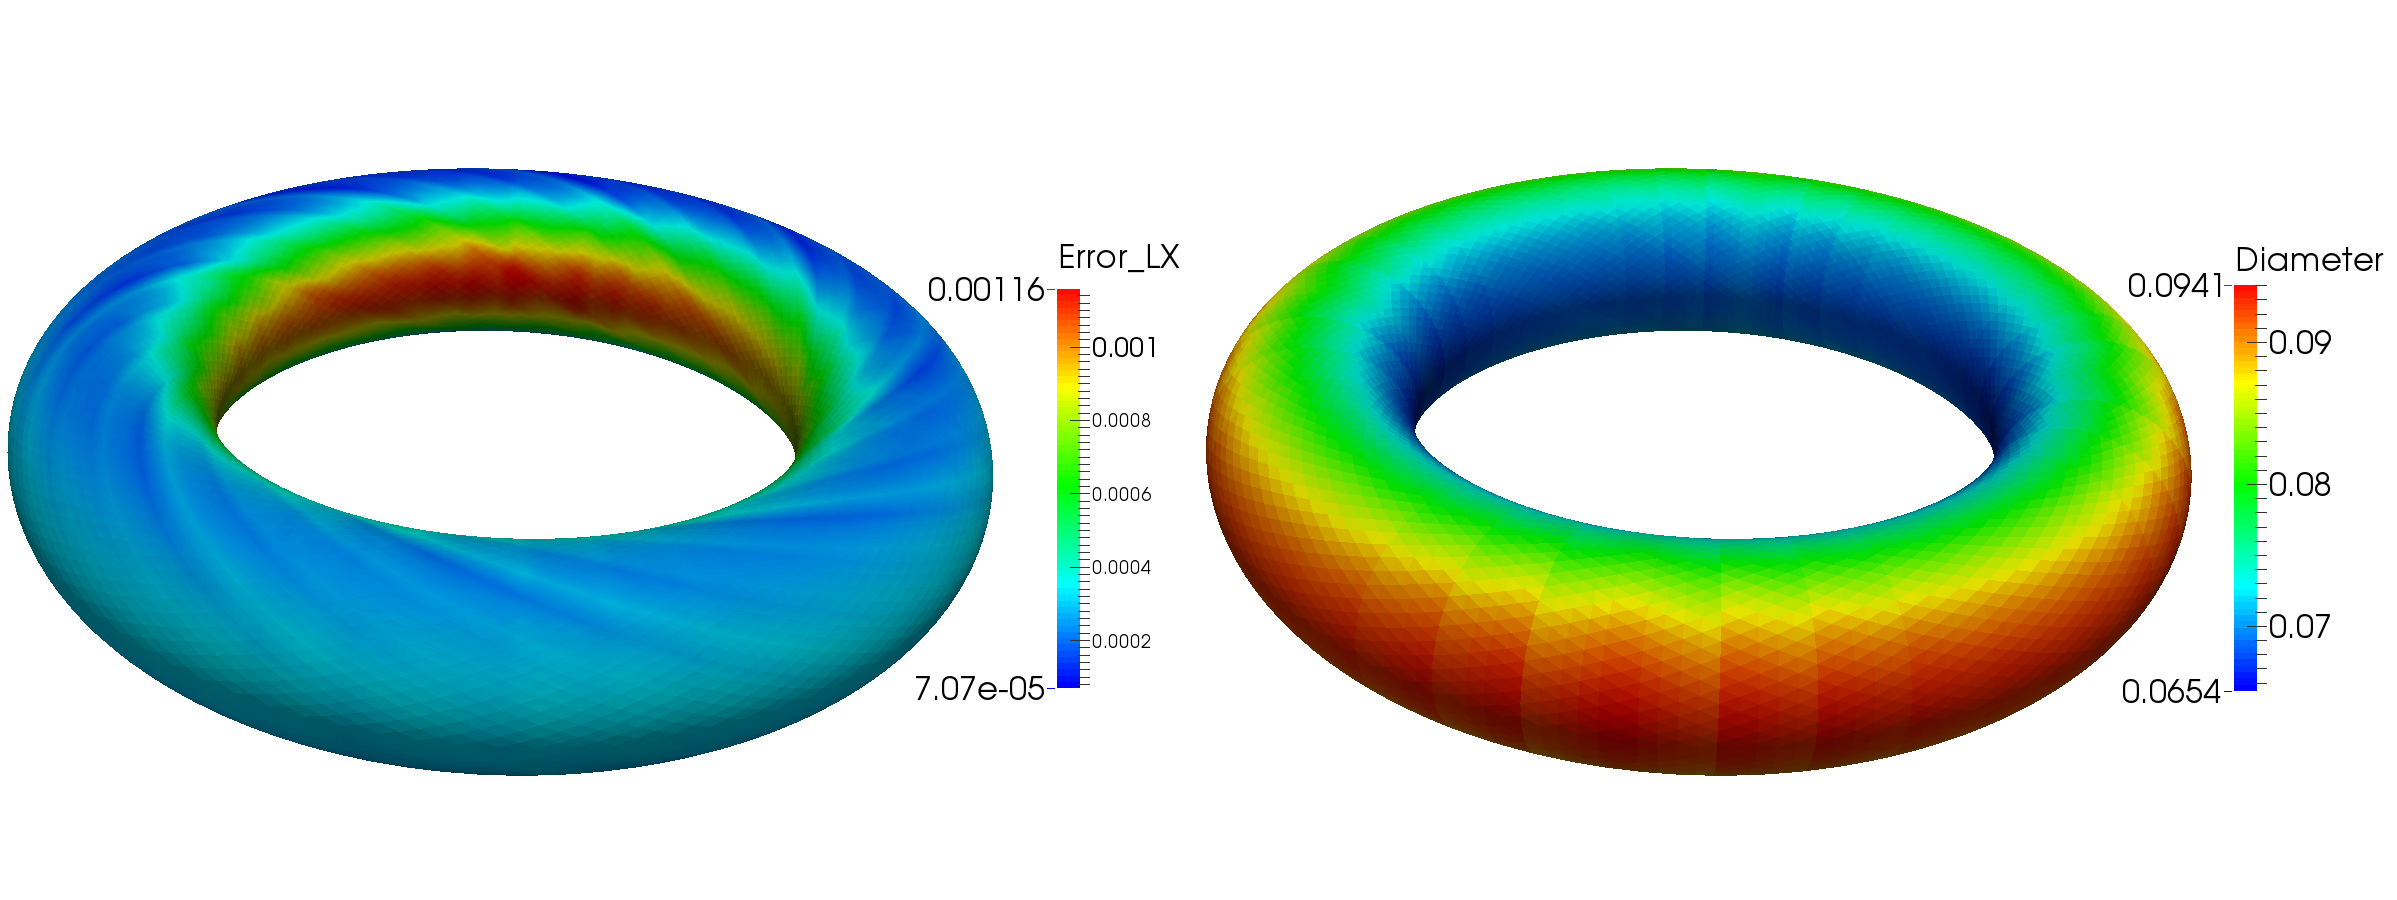
\includegraphics[width=\textwidth]{bilder/Curvature/LXDiameterTorus.png}
    \caption[Diameter u. Fehler f. Krümmungsvektor (Torus)]
            {Absolute lokale Fehler für die mittlere Krümmung berechnet aus dem Krümmungsvektor (links) und die Umkreisdurchmesser der
            Dreieckselemente (rechts).}
    \label{figLXDiameterTorus}
  \end{figure}

  \begin{figure}
    \begin{minipage}[t]{0.49\textwidth}
       \centering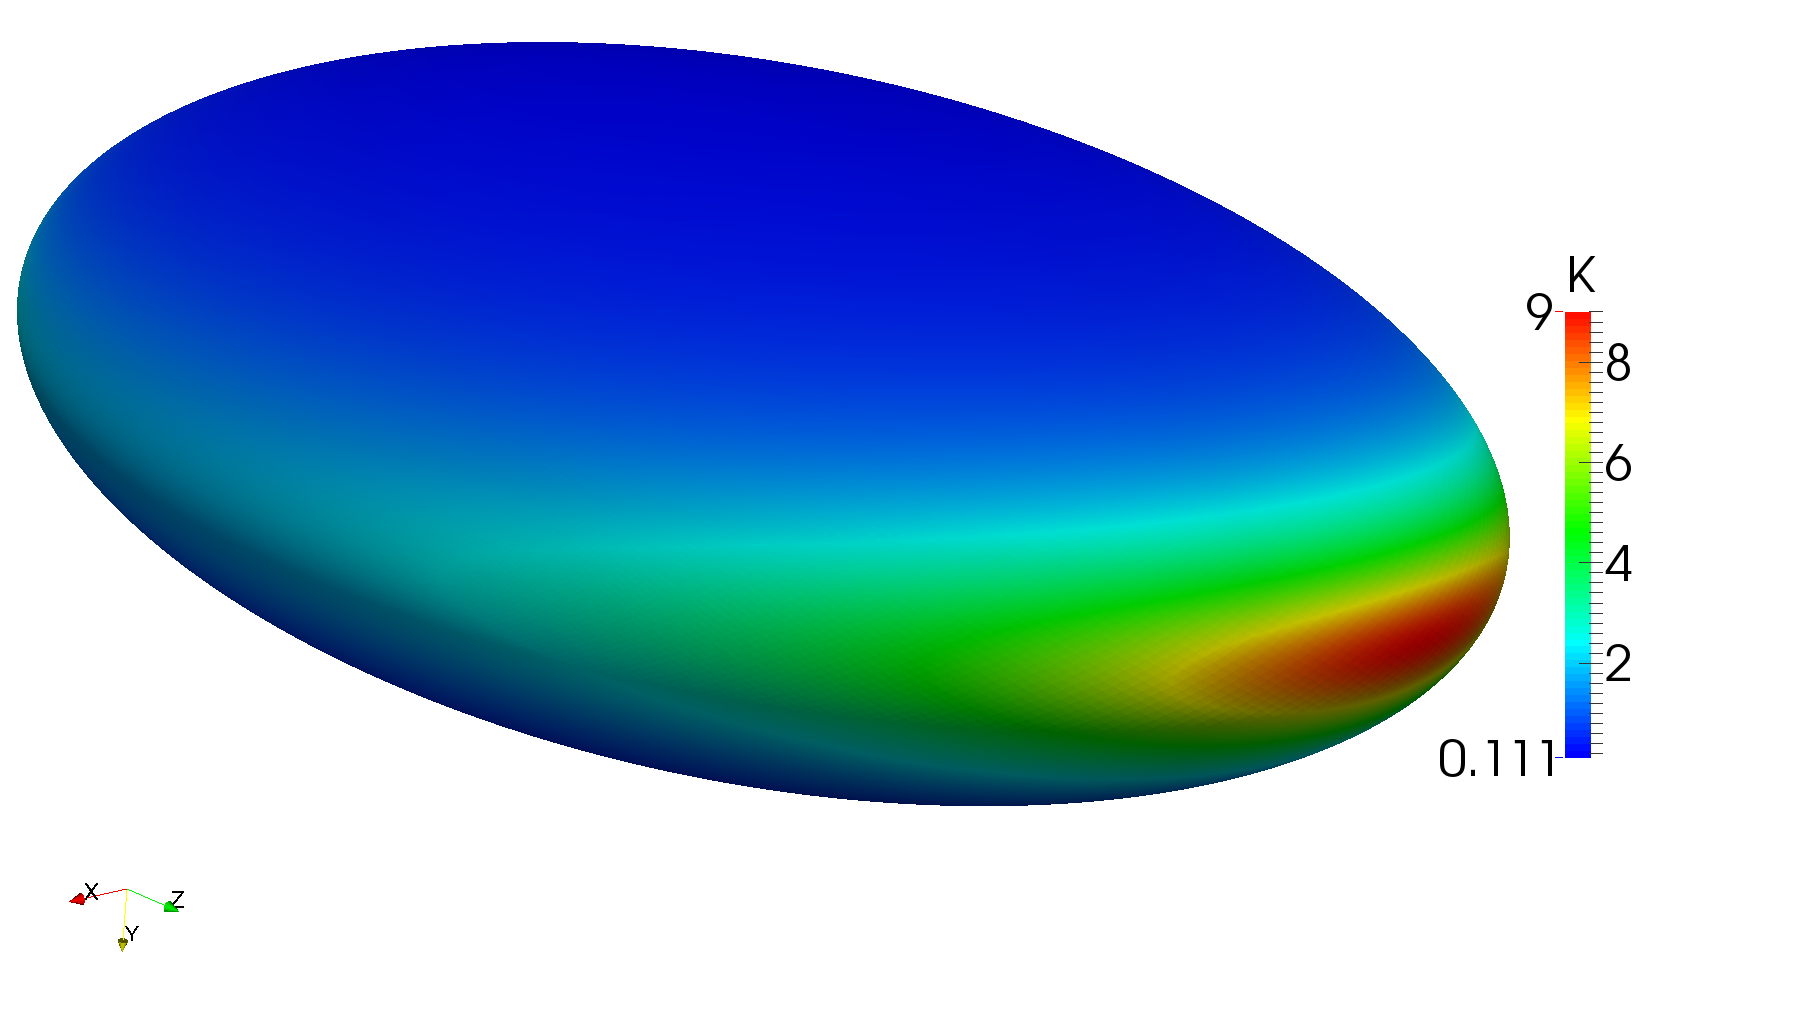
\includegraphics[width=\textwidth]{bilder/Curvature/heineC/K2k.png}
    \end{minipage}\hfill
    \begin{minipage}[t]{0.49\textwidth}
       \centering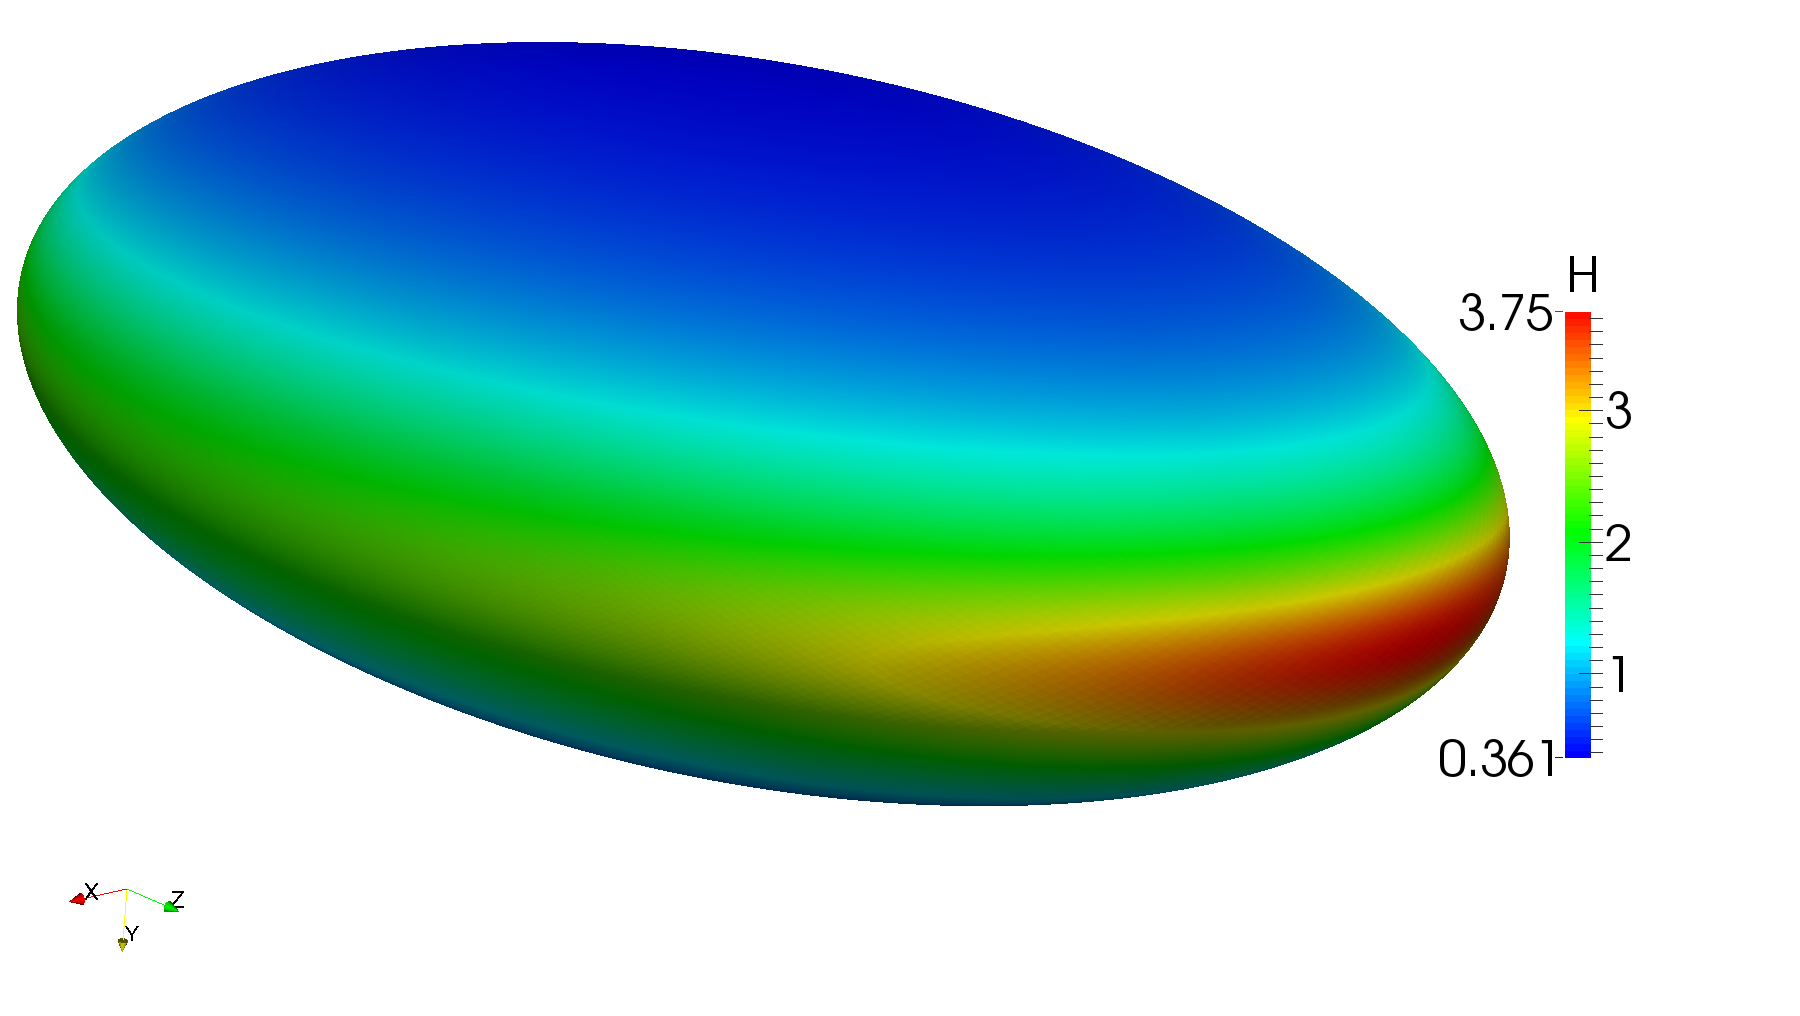
\includegraphics[width=\textwidth]{bilder/Curvature/heineC/H2k.png}
    \end{minipage}\\
    \begin{minipage}[t]{0.49\textwidth}
       \centering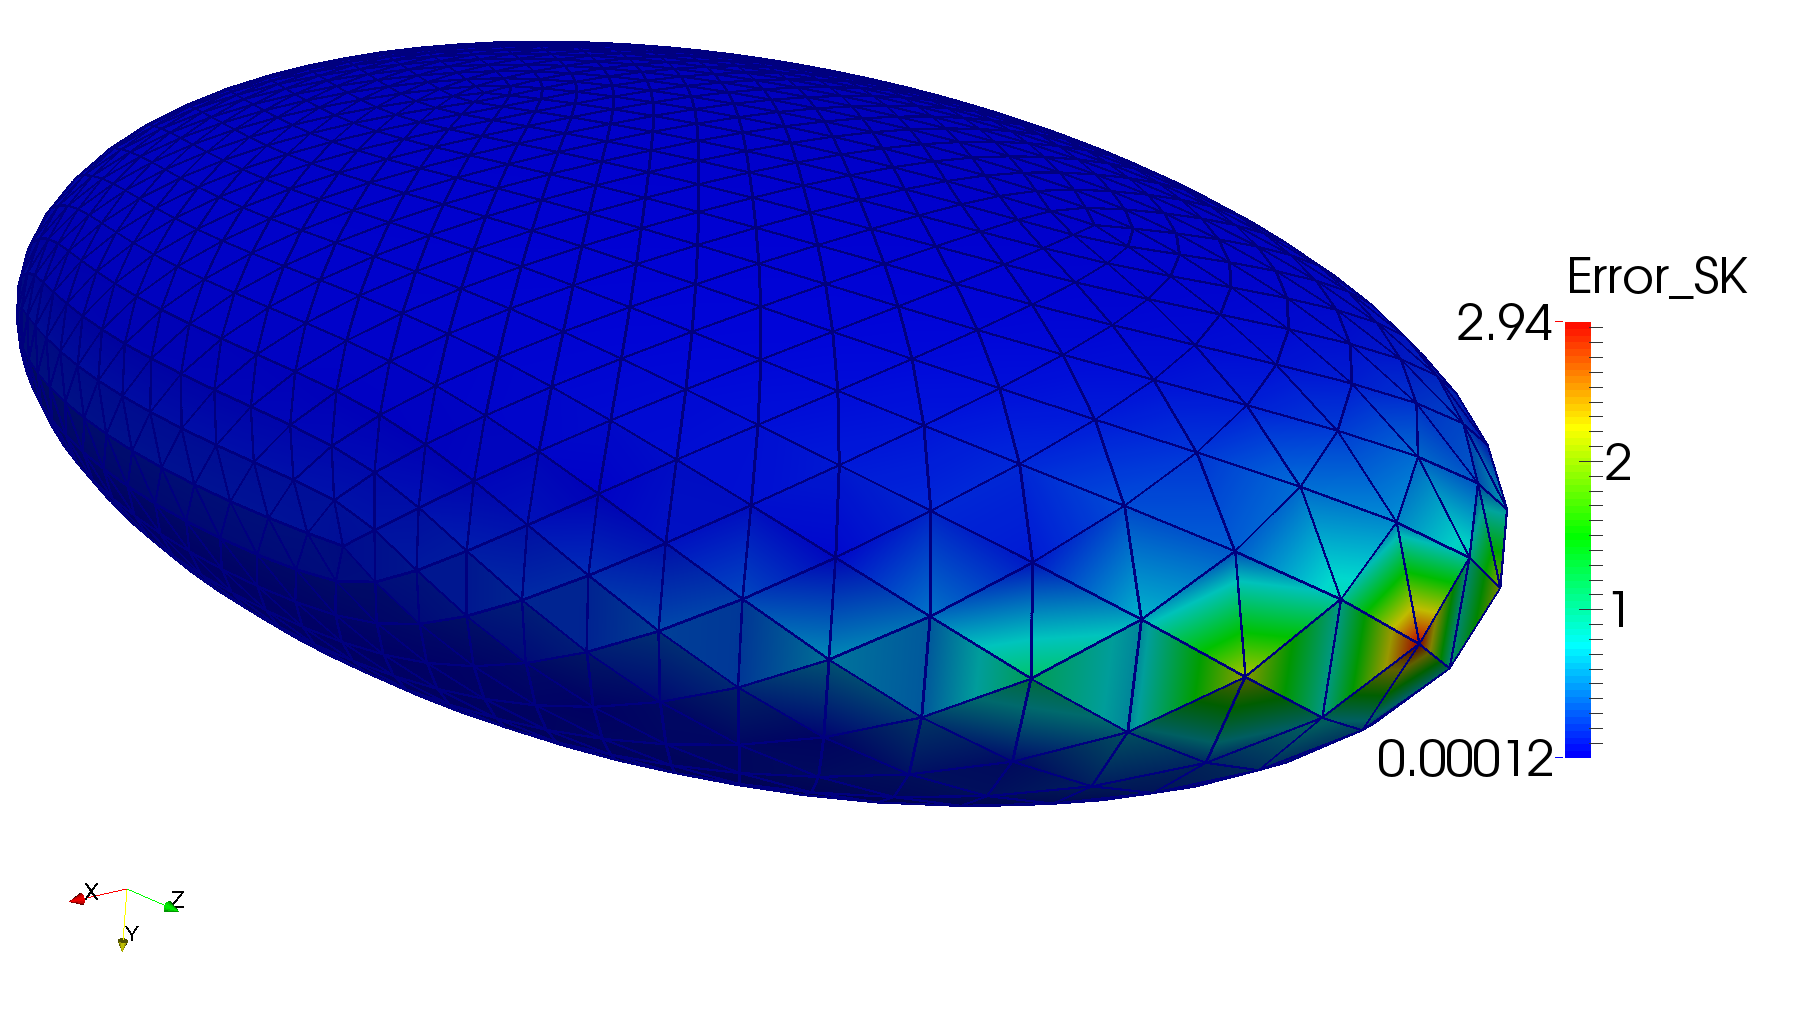
\includegraphics[width=\textwidth]{bilder/Curvature/heineC/SK2k.png}
    \end{minipage}\hfill
    \begin{minipage}[t]{0.49\textwidth}
       \centering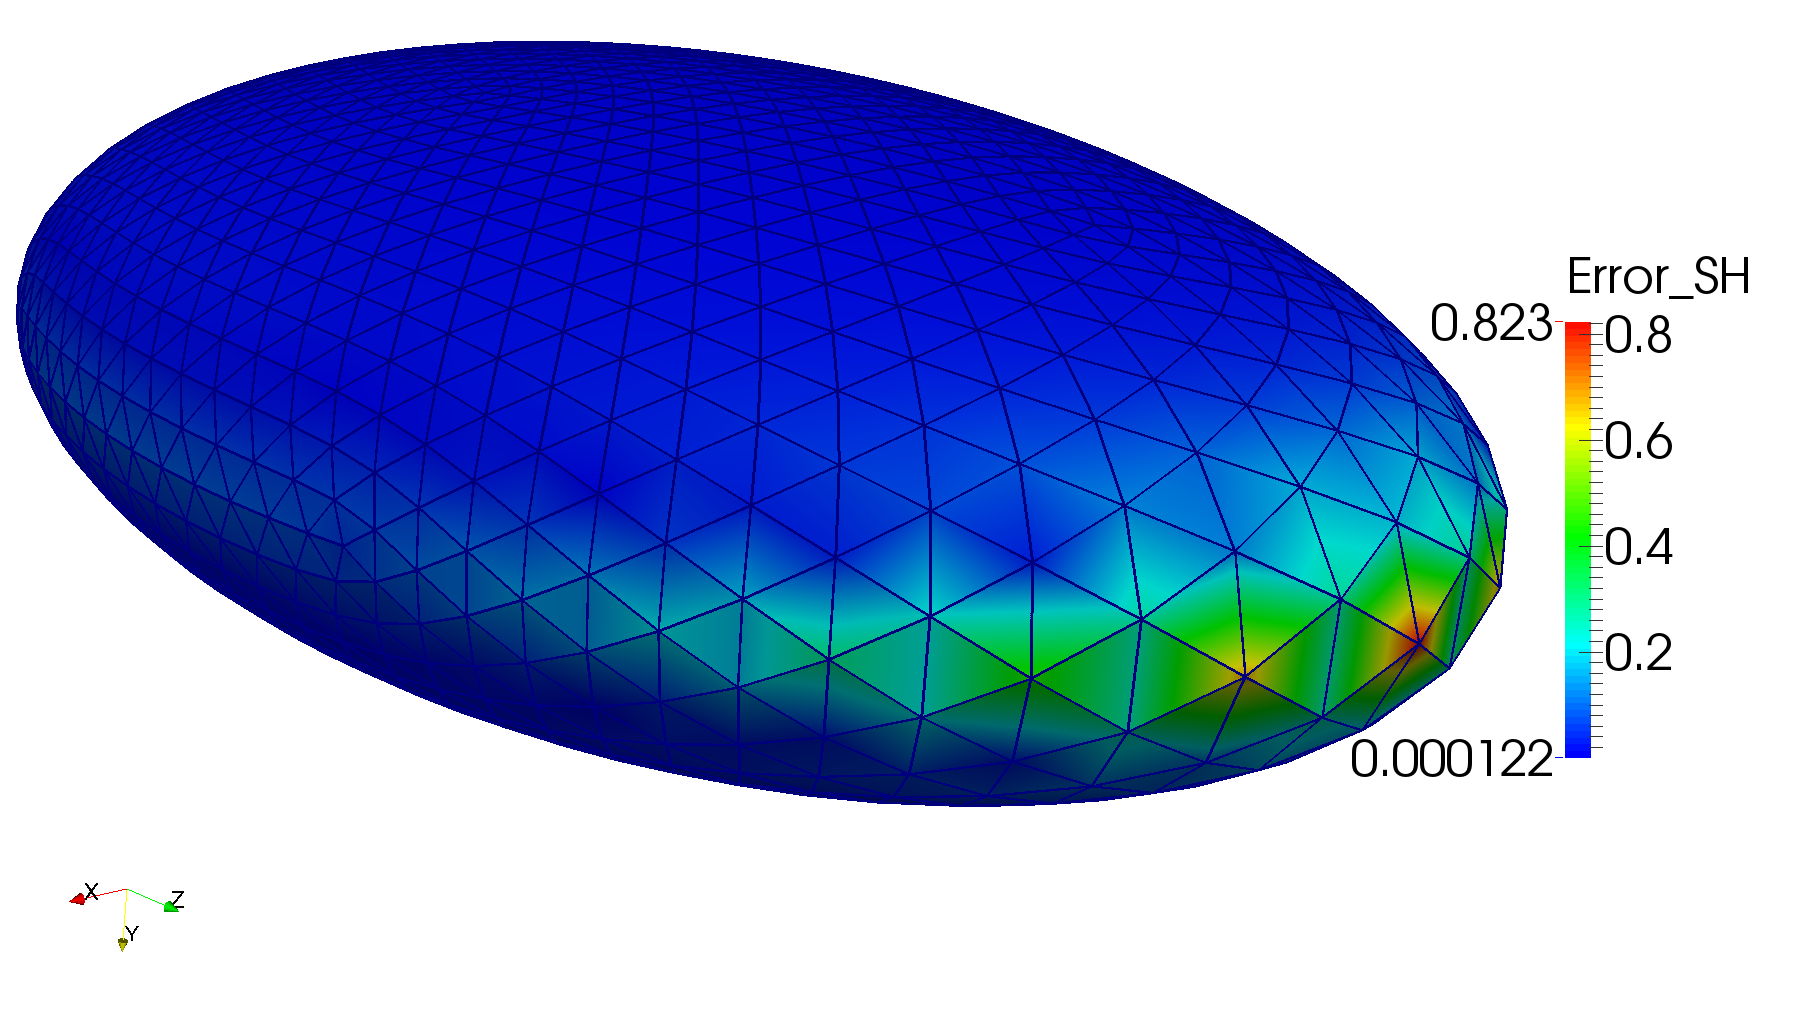
\includegraphics[width=\textwidth]{bilder/Curvature/heineC/SH2k.png}
    \end{minipage}\\
    \begin{minipage}[t]{0.49\textwidth}
       \centering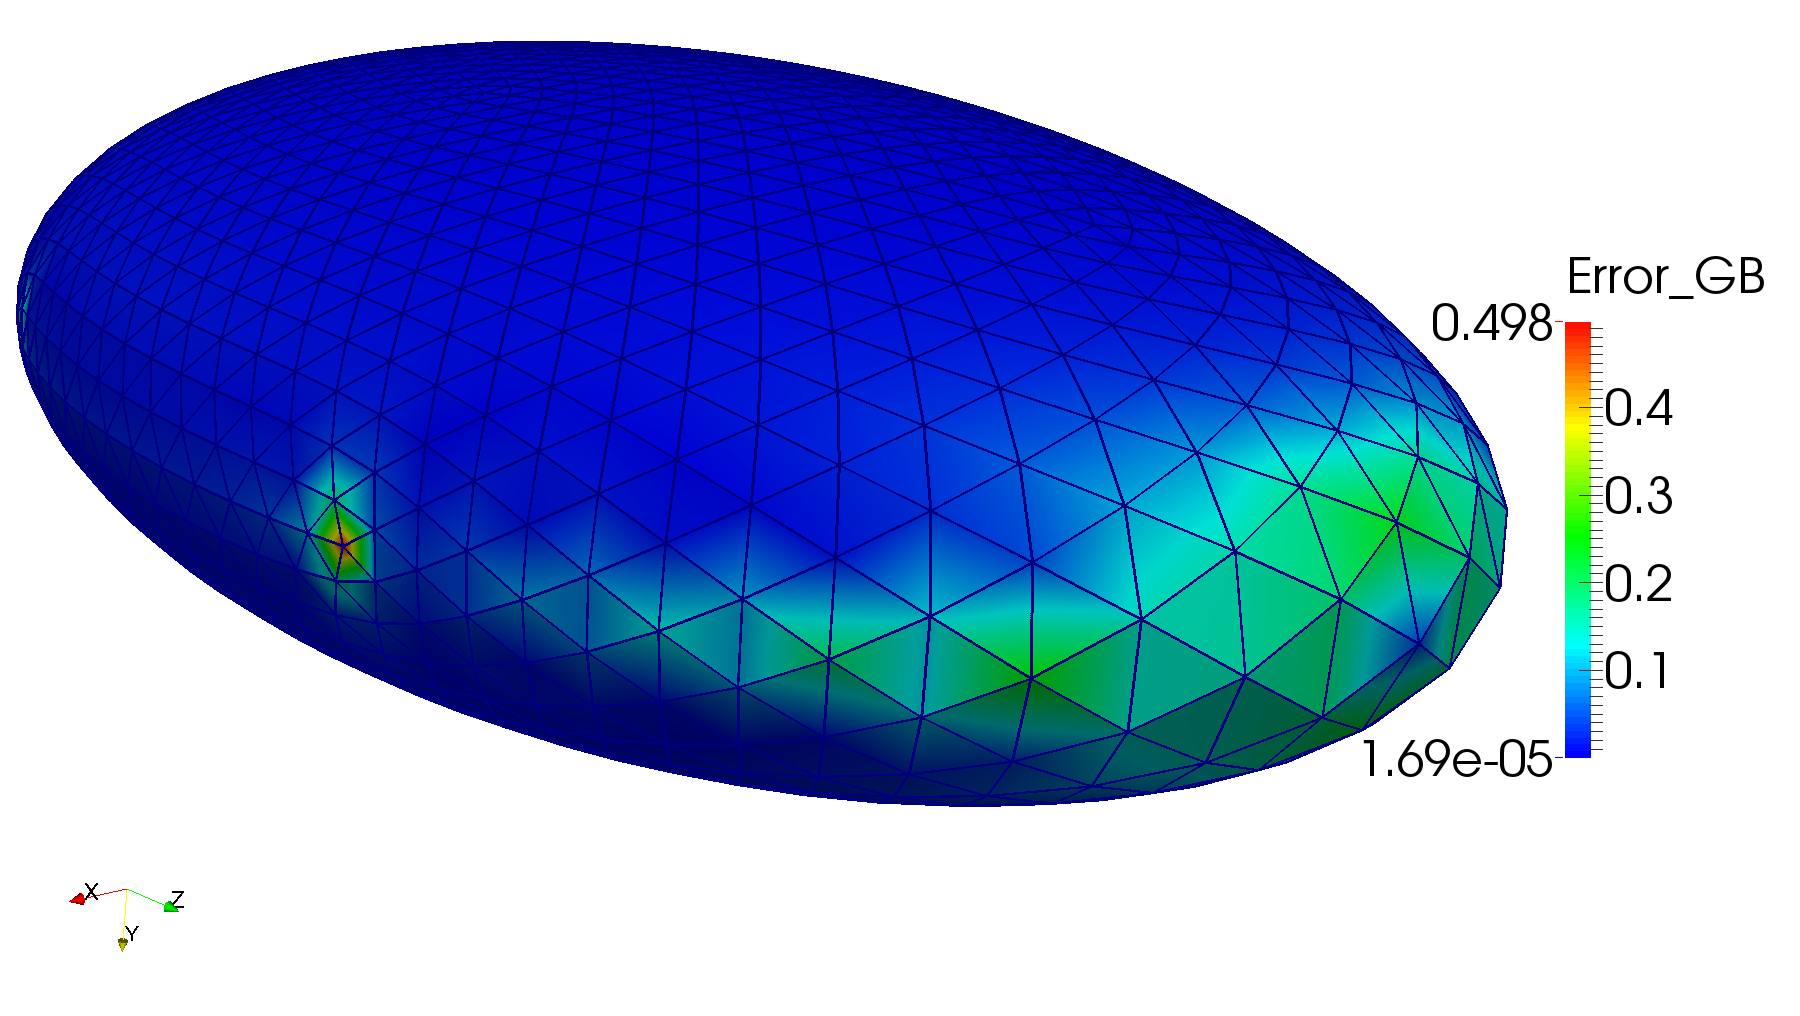
\includegraphics[width=\textwidth]{bilder/Curvature/heineC/GB2k.png}
    \end{minipage}\hfill
    \begin{minipage}[t]{0.49\textwidth}
       \centering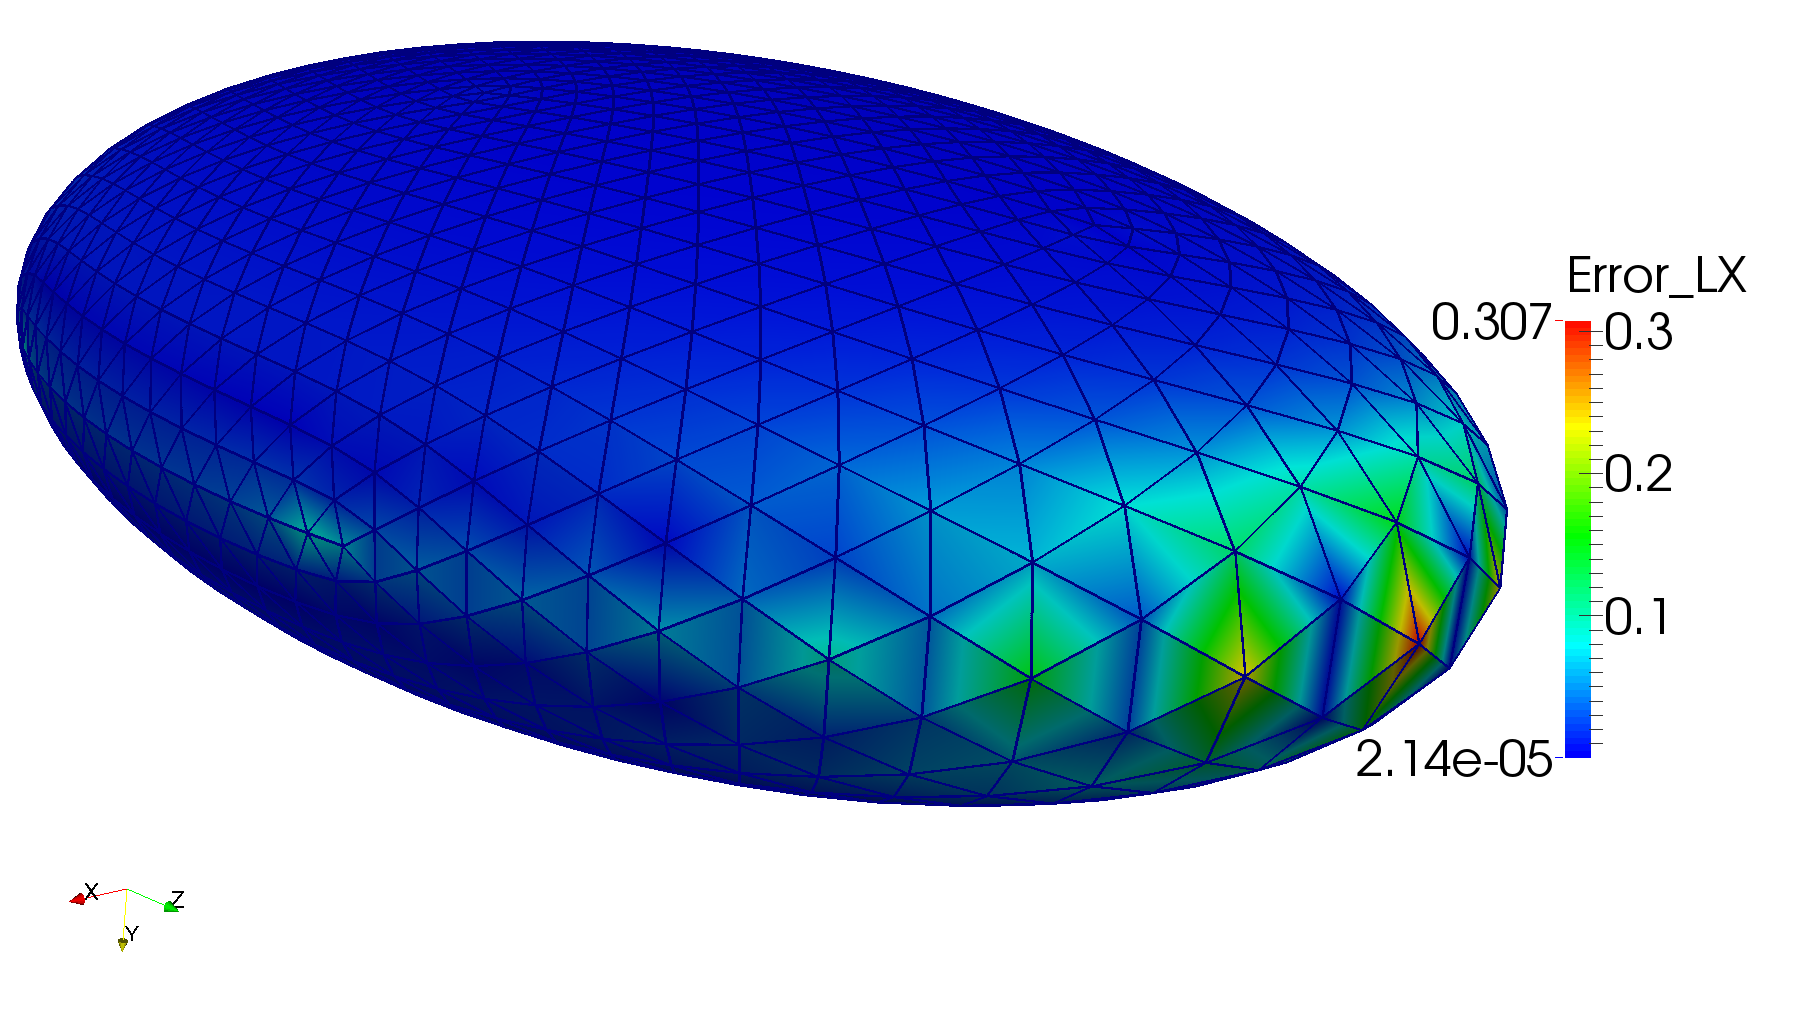
\includegraphics[width=\textwidth]{bilder/Curvature/heineC/LX2k.png}
    \end{minipage}
    \caption[Fehler (Krümmungen auf Ellipsoid)]
            {Absolute lokale Fehler für die Gaußsche Krümmung (links) und mittlere Krümmung (rechts) auf
            einem Ellipsoid
             ermittelt aus den Eigenwerten der diskreten Weingartenabbildung (Mitte), dem
             Gauß-Bonnet-Operator (unten links) bzw. dem Krümmungsvektor (unten rechts).
             (1962 DOFs, \( h\approx0.18 \))}
    \label{figErrCurvHeineC}
  \end{figure}

  \begin{figure}
    \begin{minipage}[t]{0.49\textwidth}
       \centering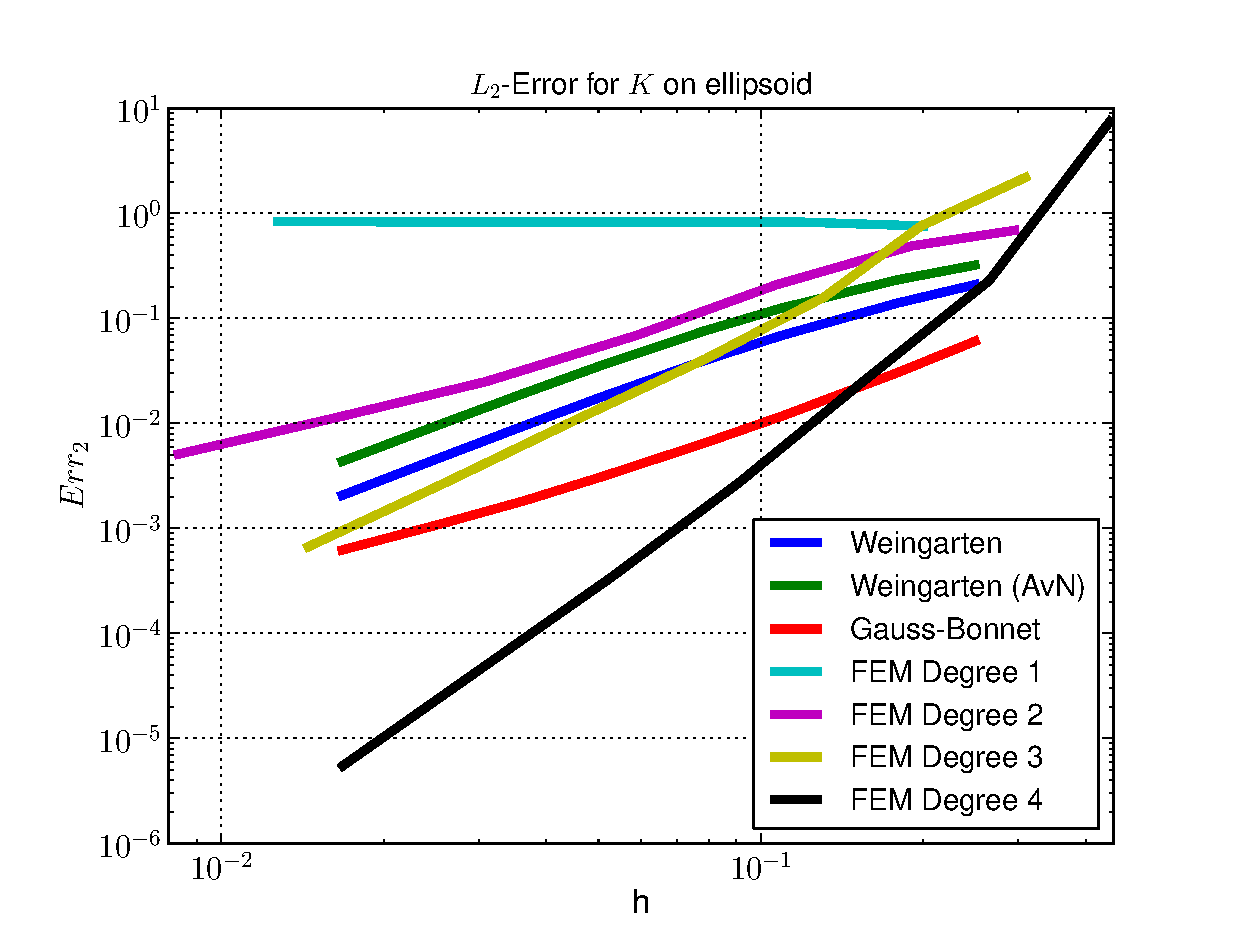
\includegraphics[width=\textwidth]{bilder/Curvature/heineC/ErrKL2.eps}
    \end{minipage}\hfill
    \begin{minipage}[t]{0.49\textwidth}
       \centering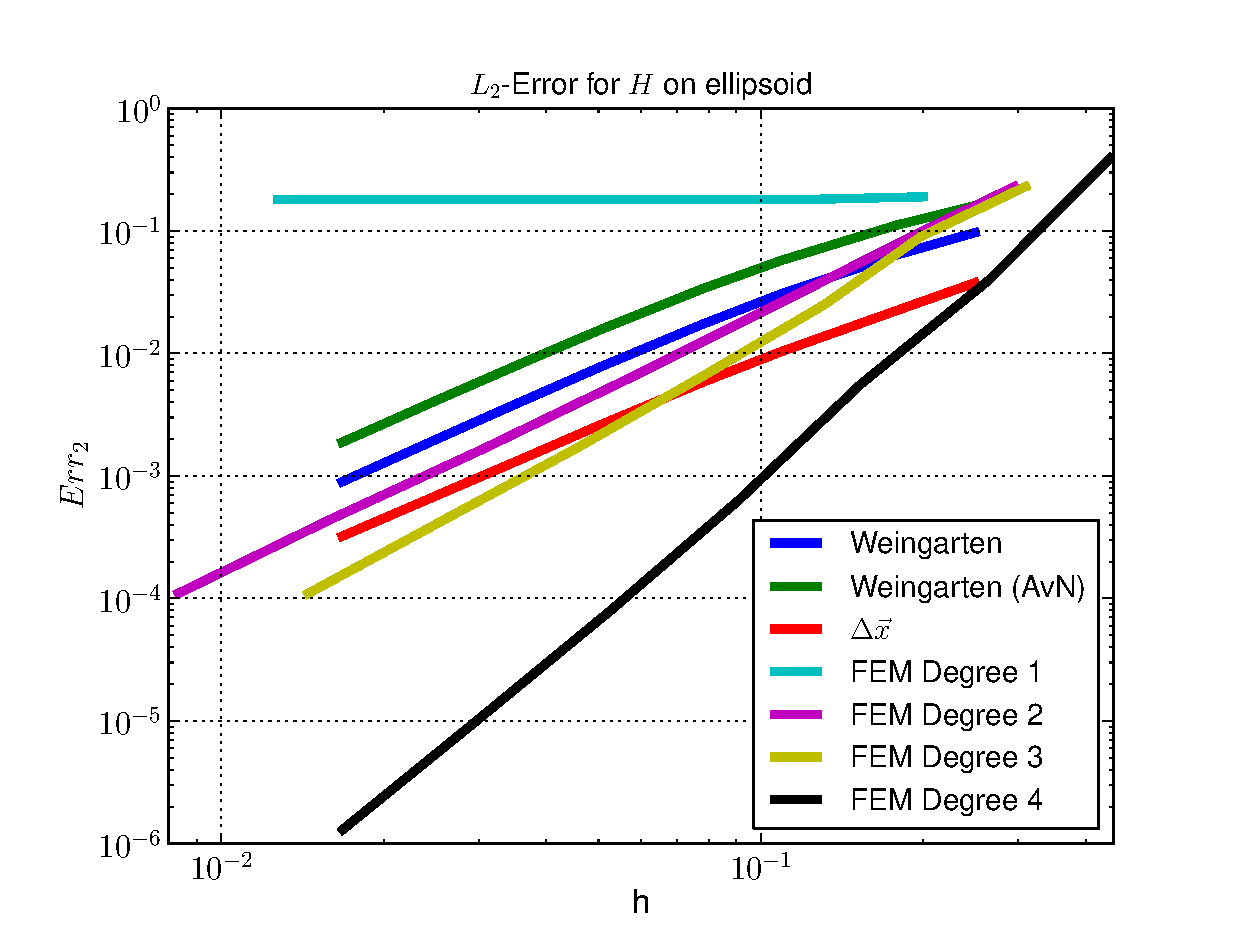
\includegraphics[width=\textwidth]{bilder/Curvature/heineC/ErrHL2.eps}
    \end{minipage}\\
    \begin{minipage}[t]{0.49\textwidth}
       \centering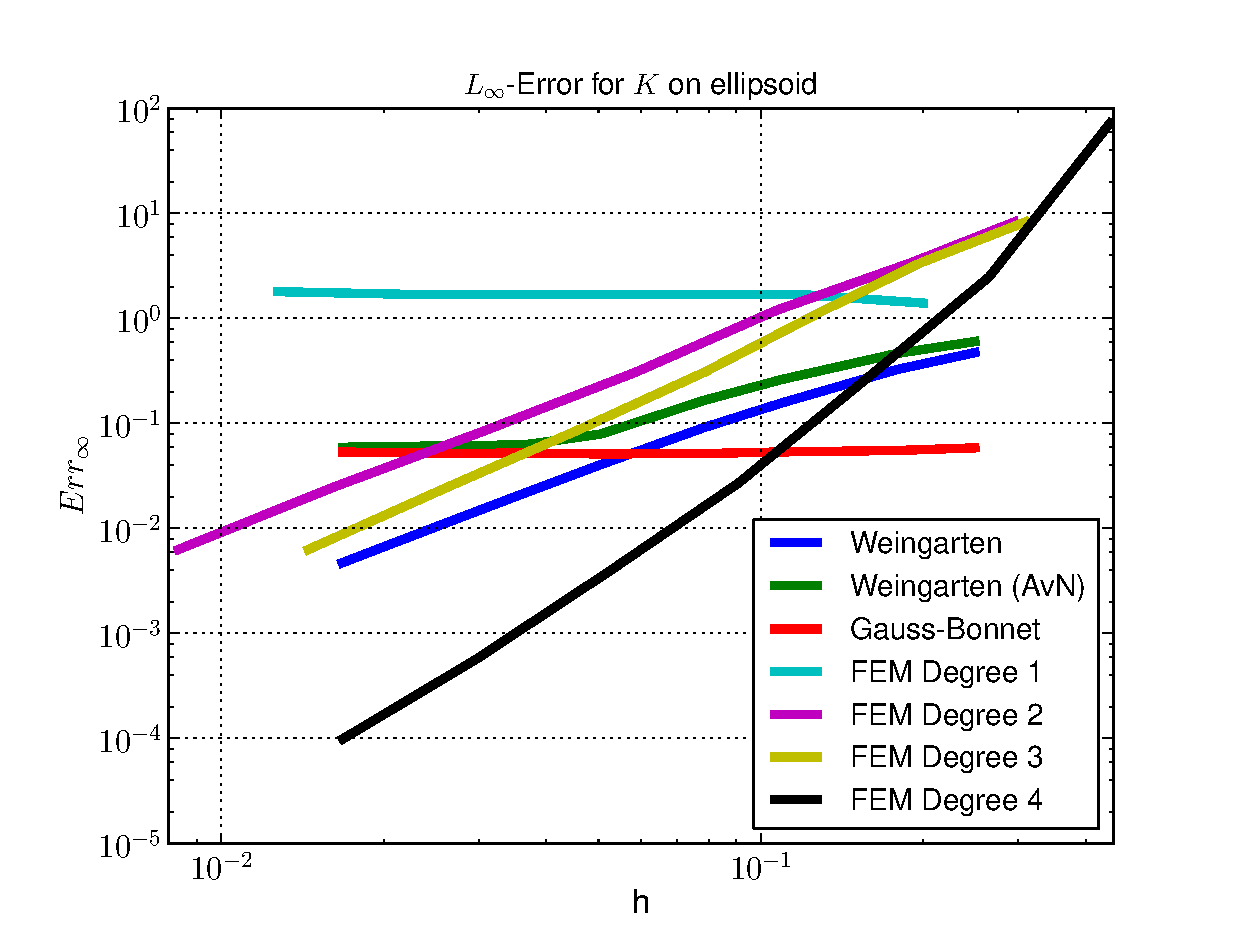
\includegraphics[width=\textwidth]{bilder/Curvature/heineC/ErrKMax.eps}
    \end{minipage}\hfill
    \begin{minipage}[t]{0.49\textwidth}
       \centering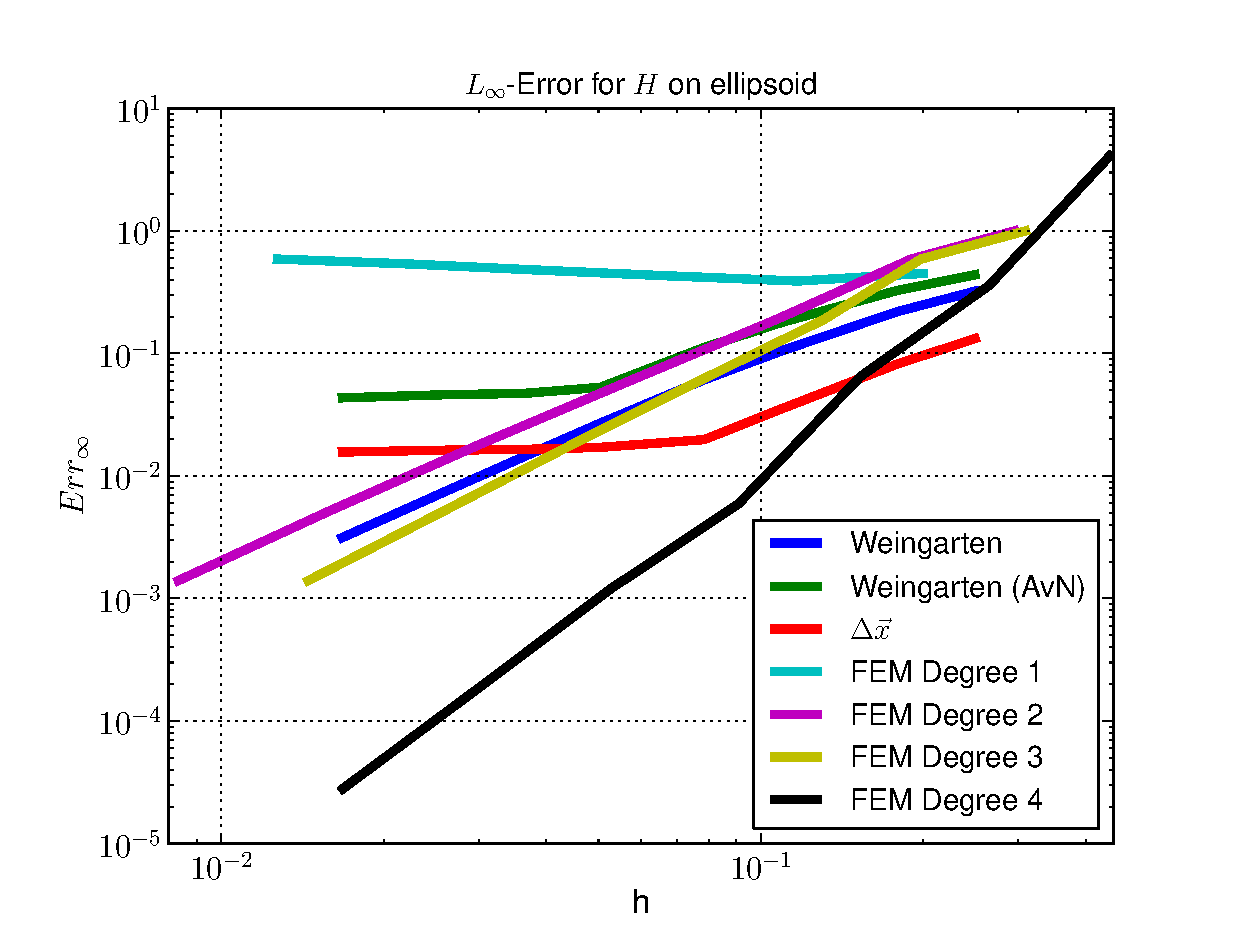
\includegraphics[width=\textwidth]{bilder/Curvature/heineC/ErrHMax.eps}
    \end{minipage}
    \caption[Fehlerplot (Krümmungen auf Ellipsoid)]
            {Log-Log-Plot der relativen diskreten \( L_{2} \)-Fehler (oben) und Maximumsfehler (unten) 
             für die Gaußsche Krümmung (links) und mittlere Krümmung (rechts) auf einem Ellipsoid.}
    \label{figErrCompHeineC}
  \end{figure}
